 %--------------------------------------------------------------------%
% Berkas utama template LaTeX.
% author Petra Barus, Peb Ruswono Aryan - Dionesius Agung (2020)
%--------------------------------------------------------------------%

\documentclass[12pt, a4paper, onecolumn, oneside, final]{report}

%-------------------------------------------------------------------%
%
% Konfigurasi dokumen LaTeX untuk laporan tesis IF ITB
%
% @author Petra Novandi
% updated by Dionesius Agung (2020)
%-------------------------------------------------------------------%
%
% Berkas asli berasal dari Steven Lolong
%
%-------------------------------------------------------------------%

\usepackage[top=3cm,bottom=3cm,left=4cm,right=3cm,a4paper]{geometry}

\usepackage[english]{babel}

\renewcommand{\baselinestretch}{1.5}


%%%%%%%%%%%%%%%%%%%%%%%%%%%%%%%
%  BIBLIOGRAPHY AND CITATION  %
%%%%%%%%%%%%%%%%%%%%%%%%%%%%%%%
% use package biblatex
\usepackage[backend=biber,natbib,
            bibstyle=authoryear,
            citestyle=authoryear,
            sorting=nyt,
            url=false,
            maxcitenames=2,
            maxnames=2,
            dashed=false,
            uniquename=init,
            giveninits=true]{biblatex}
\DeclareNameAlias{author}{family-given}

% Translate bibliography strings ke bahasa indonesia
%   (karena 'bahasa' belum di-support)
\DefineBibliographyStrings{english}{%
  bibliography = {Daftar Pustaka},
  references = {Referensi},
  and = {\&},
  techreport = {Dok. teknis},
  phdthesis = {Disertasi doktoral\adddot},
  andothers = {dkk\adddot}
}

% Field berikut tidak ditulis di daftar pustaka
\AtEveryBibitem{\clearfield{issn}}
\AtEveryBibitem{\clearfield{isbn}}
\AtEveryBibitem{\clearfield{month}}
\AtEveryBibitem{\clearfield{doi}}

% Format entri daftar pustaka

%% Beri titik setelah judul
\DeclareFieldFormat
[article,inbook,incollection,inproceedings,
patent,unpublished,misc]
{title}{#1\isdot}

%% Judul buku ditulis italic
\DeclareFieldFormat
[thesis]
{title}{\emph{#1}\isdot}

%% Hilangkan kata "Dalam:" di antara judul artikel dan judul jurnal
\renewbibmacro{in:}{}

%% Format penulisan volume dan nomor pada jurnal: vol(num) e.g. 5(1)
\renewbibmacro*{volume+number+eid}{%
	\printfield{volume}%
	\printfield{number}%
	\setunit{\addcomma\space}%
	\printfield{eid}}
\DeclareFieldFormat[article]{number}{\mkbibparens{#1}}

% Format citation
\renewcommand*{\nameyeardelim}{\addcomma\space}

% Setting spasi di halaman daftar pustaka
\setlength\bibitemsep{0.5\baselineskip}


%%%%%%%%%%%%%%
%  PACKAGES  %
%%%%%%%%%%%%%%
\usepackage[utf8]{inputenc}
\usepackage{csquotes}
\usepackage{bookmark}
\usepackage{graphicx}
\usepackage{titling}
\usepackage{blindtext}
\usepackage{sectsty}
\usepackage{chngcntr}
\usepackage{etoolbox}
\usepackage{hyperref}       % Package untuk link di daftar isi.
\usepackage{titlesec}       % Package Format judul
\usepackage{parskip}
\usepackage{pdflscape}
\usepackage{afterpage}
\usepackage{ltablex}
\usepackage{booktabs}
\usepackage{tabularx}
\usepackage{multirow}
\usepackage[table,xcdraw]{xcolor}


%%%%%%%%%%%%%%$$%%%%%%%%%
%  CHAPTER AND SECTION  %
%%%%%%%%%%%%%%%%$$%%%%%%%
% Format judul bab
\chapterfont{\centering \large}
\titleformat{\chapter}[display]
  {\large\centering\bfseries}
  {\chaptertitlename\ \thechapter}{0em}
    {\large\bfseries\MakeUppercase}
\titlespacing*{\chapter}
	{0pt}
	{-1.5\baselineskip}
	{1.5\baselineskip}

% Format judul section (dan sub(sub)section)
\titleformat*{\section}{\bfseries\normalsize}
\titleformat*{\subsection}{\bfseries\normalsize}
\titleformat*{\subsubsection}{\bfseries\normalsize}
\titlespacing*{\section}{0pt}{1ex}{0pt}
\titlespacing*{\subsection}{0pt}{1ex}{0pt}
\titlespacing*{\subsubsection}{0pt}{1ex}{0pt}

% Kedalaman hierarki section (paling dalam subsubsection)
\setcounter{secnumdepth}{3}

\hbadness=99999
\vbadness=99999

%%%%%%%%%%%%%%%%%%%%%%%%%%%%%%%%%%%%%%%%%%%%%%%%%%
%  TABLE OF CONTENTS, LISTS OF FIGURES & TABLES  %
%%%%%%%%%%%%%%%%%%%%%%%%%%%%%%%%%%%%%%%%%%%%%%%%%%
\usepackage[titles]{tocloft}
% \usepackage[titletoc]{appendix}
\usepackage{tocbibind}

% Kedalaman hierarki maksimum ToC
% (yang masuk ToC hanya sampai subsection: I.1.1.)
\setcounter{tocdepth}{2}

% Hilangkan gap antar-bab di ToC
\setlength{\cftbeforechapskip}{0pt}

% Tambah kata "BAB" sebelum nomor bab di daftar isi
% TODO: still problematic when used with list of appendices (uncomment these 4 following lines to reproduce the problem)
\renewcommand{\cftchappresnum}{BAB~} % BAB before number in ToC
\newlength{\mylen} % a scratch length
\settowidth{\mylen}{\bfseries\cftchappresnum\cftchapaftersnum} % extra space
\addtolength{\cftchapnumwidth}{\mylen} % add the extra space

\renewcommand{\cftchapleader}{\cftdotfill{\cftdotsep}}

% Pisah daftar lampiran dari ToC
%%%
% \renewcommand{\appendixtocname}{Daftar Lampiran}

% \makeatletter
% \let\oldappendix\appendices

% \renewcommand{\appendices}{%
%   \clearpage
%   % From now, everything goes to the app file and not to the toc
%   \let\tf@toc\tf@app
%   \addtocontents{app}{\protect\setcounter{tocdepth}{1}}
%   \immediate\write\@auxout{%
%     \string\let\string\tf@toc\string\tf@app^^J
%   }
%   \oldappendix
% }%

\newcommand{\listofappendices}{%
  \begingroup
  \renewcommand{\contentsname}{\appendixtocname}
  \let\@oldstarttoc\@starttoc
  \def\@starttoc##1{\@oldstarttoc{app}}
  % Reusing the code for \tableofcontents with different
  %   \contentsname and different file handle app
  \tableofcontents
  \endgroup
}
\makeatother
%%%

% Hilangkan gap antara entri gambar & tabel antarbab di daftar tabel 
% dan daftar gambar (hanya terlihat kalau ada gambar/tabel di >1 bab)
\newcommand*{\noaddvspace}{\renewcommand*{\addvspace}[1]{}}
\addtocontents{lof}{\protect\noaddvspace}
\addtocontents{lot}{\protect\noaddvspace}


%%%%%%%%%%%%%%%%%%%%%%%%%%%%%%%%%%%%%%%%%
%  FLOATS: FIGURES, TABLES, ALGORITHMS  %
%%%%%%%%%%%%%%%%%%%%%%%%%%%%%%%%%%%%%%%%%
% Before:
% ---
% Counter untuk figure dan table.
% \counterwithin{figure}{section}
% \counterwithin{table}{section}
% ---
\renewcommand\dateenglish{%
 \def\today{\number\day\space\ifcase\month\or
    Januari\or Februari\or Maret\or April\or Mei\or Juni\or
    Juli\or Agustus\or September\or Oktober\or November\or
    Desember\fi
    \space\number\year}}
\def\thismonth{\ifcase\month\or
Januari\or Februari\or Maret\or April\or Mei\or Juni\or
Juli\or Agustus\or September\or Oktober\or November\or
Desember\fi
\space\number\year}

\usepackage[labelsep=period,
justification=justified,
format=hang,
figurename=Gambar,
tablename=Tabel]{caption}
\usepackage[labelformat=simple]{subcaption}
%% Hack subfigure cross-ref agar pakai tanda kurung
%%   e.g. Gambar II.2(a), bukan Gambar II.2a
%% (method recommended in subcaption package documentation)
\renewcommand\thesubfigure{(\alph{subfigure})}

% Counter untuk gambar dan tabel
\renewcommand*{\thefigure}{\thechapter.\arabic{figure}}
\renewcommand*{\thetable}{\thechapter.\arabic{table}}

% Jarak spasi antara float dengan teks utama
\captionsetup[figure]{belowskip=-1em}
% \captionsetup[subfigure]{belowskip=0pt}
\setlength{\textfloatsep}{2\baselineskip}
\setlength{\intextsep}{2\baselineskip}

% Spasi single di environment table
\AtBeginEnvironment{table}
  {\renewcommand{\baselinestretch}{1.0}}

% Avoid widow and orphan lines if possible
\widowpenalty500
\clubpenalty10000

% Hyphenation penalty
\hyphenpenalty=10000
\tolerance=1
\sloppy

\usepackage[chapter]{algorithm}
\usepackage{algpseudocode}
% Rename "Algorithm" into "Algoritma"
\makeatletter
\renewcommand*{\ALG@name}{Algoritma}
\newcommand{\algorithmname}{\ALG@name}
\makeatother


%%%%%%%%%%%%%%%%%%%%%%%%%
%  MATHS AND EQUATIONS  %
%%%%%%%%%%%%%%%%%%%%%%%%%
\usepackage{amsmath}
\usepackage{amsfonts}
\usepackage{mathtools}

% Counter untuk equation
\renewcommand*{\theequation}{\thechapter.\arabic{equation}}

% Allow page breaks on long equations
\allowdisplaybreaks[1-4]

\makeatletter
\makeatother

\addbibresource{references.bib}

\begin{document}
%Basic configuration
\title{Pelacakan Objek Dinamis Menggunakan Pengukuran Banyak Agen dengan Latensi Komunikasi pada Robot Kontes Sepak Bola Beroda}
\date{\today}
\author{
    Bimo Adityarahman Wiraputra \\
    NIM: 13517004
}

\pagenumbering{roman}
\setcounter{page}{0}

\clearpage
\pagestyle{empty}

\newgeometry{top=3cm,bottom=3cm,left=3cm,right=3cm}

{\fontfamily{ptm}\selectfont%
    \begin{center}

        \smallskip

        \large{\bfseries \MakeUppercase{\thetitle}}
        \\[2\baselineskip]

        \large{\bfseries Laporan Tugas Akhir}
        \\[\baselineskip]

        \normalsize{ \bfseries
            Disusun sebagai syarat kelulusan tingkat sarjana
        }
        \\[3\baselineskip]

        \normalsize{ \bfseries Oleh\\}
        \large{ \bfseries \MakeUppercase{\theauthor}}

        \vfill
        \begin{figure}[h]
            \centering
            \includegraphics[height=3.5cm,keepaspectratio]{resources/cover-ganesha.jpg}
        \end{figure}
        \vfill

        \large{ \bfseries
            \uppercase{
                Program Studi Teknik Informatika \\
                Sekolah Teknik Elektro dan Informatika \\
                Institut Teknologi Bandung\\
            }
            \thismonth
        }

    \end{center}
}%

\restoregeometry
\clearpage

\clearpage
\pagestyle{empty}

\begin{center}

    \large{\bfseries \MakeUppercase{\thetitle}}
    \\[2\baselineskip]

    \large{\textbf{Laporan Tugas Akhir}}
    \\[2\baselineskip]

    \normalsize{Oleh\\
        \MakeUppercase{\textbf{\theauthor}}\\
        \textbf{Program Studi Teknik Informatika} \\
        Sekolah Teknik Elektro dan Informatika \\
        Institut Teknologi Bandung}
    \\[3\baselineskip]


    \normalsize{
        Telah disetujui dan disahkan sebagai Laporan Tugas Akhir \\
        di Bandung, pada tanggal \today \\
        Mengetahui, \\[1\baselineskip]
        Pembimbing,\\[4\baselineskip]
        \underline{Dr. Judhi Santoso, M.Sc.}\\
        NIP. 196302041989031002}

\end{center}
\clearpage

\chapter*{Lembar Pernyataan}

Dengan ini saya menyatakan bahwa:

\begin{enumerate}

    \item Pengerjaan dan penulisan Laporan Tugas Akhir ini dilakukan tanpa menggunakan bantuan yang tidak dibenarkan.
    \item Segala bentuk kutipan dan acuan terhadap tulisan orang lain yang digunakan di dalam penyusunan laporan tugas akhir ini telah dituliskan dengan baik dan benar.
    \item Laporan Tugas Akhir ini belum pernah diajukan pada program pendidikan di perguruan tinggi mana pun.

\end{enumerate}

Jika terbukti melanggar hal-hal di atas, saya bersedia dikenakan sanksi sesuai dengan Peraturan Akademik dan Kemahasiswaan Institut Teknologi Bandung bagian Penegakan Norma Akademik dan Kemahasiswaan khususnya Pasal 2.1 dan Pasal 2.2.
\\

Bandung, \thedate \\[4\baselineskip]
\underline{Bimo Adityarahman Wiraputra} \\
NIM 13517004


\pagestyle{plain}

\clearpage
\chapter*{Abstrak}
\addcontentsline{toc}{chapter}{ABSTRAK}

\begin{center}
	\large{\bfseries{
			\MakeUppercase\thetitle
		}
	}

	\normalsize{
		Oleh\\
		\MakeUppercase \theauthor
	}
\end{center}

\medskip

\begin{spacing}{1.0}

	\blindtext

	\blindtext

	Kata kunci: \LaTeX, tugas akhir, template, teknik informatika

\end{spacing}

\clearpage

\chapter*{Kata Pengantar}
\addcontentsline{toc}{chapter}{KATA PENGANTAR}

Puji syukur penulis panjatkan kepada Allah SWT karena hanya dengan rahmat dan karuniaNya, laporan tugas akhir yang berjudul \thetitle{} ini dapat dirampungkan dengan baik dan tepat waktu. Penulis juga mengucapkan terima kasih kepada semua pihak yang telah terlibat dan membantu penulis dalam pengerjaan tugas akhir ini, termasuk tapi tidak terbatas padanya diantaranya:

\begin{enumerate}
    \item Bapak Dr. Judhi Santoso, M.Sc. sebagai pembimbing penulis yang telah membimbing dan mengarahkan penulis dalam pengembangan solusi dan penulisan tugas akhir ini.
    \item Bapak Ir. Rila Mandala, M.Eng., Ph.D. sebagai penguji penulis yang telah memberi kritik dan saran untuk tugas akhir ini sehingga dapat menjadi lebih baik lagi.
    \item Ibu Ginar Santika Niwanputri, S.T., M.Sc., Bapak Adi Mulyanto, S.T., M.T., Bapak Nugraha Priya Utama, S.T., M.A., Ph.D., Ibu Latifa Dwiyanti, S.T., M.T., dan seluruh anggota tim tugas akhir lainnya yang telah mengatur dan mengarahkan penulis dan mahasiswa lainnya dalam pengerjaan dan penulisan tugas akhir ini.
    \item Dosen-dosen Teknik Informatika dan dosen Institut Teknologi Bandung secara umum yang telah mendidik dan memberikan ilmu kepada penulis sehingga penulis dapat mengerjakan tugas akhir ini.
    \item Kementerian Pendidikan dan Kebudayaan Indonesia yang telah membiayai penulis dalam menempuh pendidikan tinggi di Teknik Informatika ini.
    \item Keluarga penulis yang selalu mendukung penulis di dalam pengerjaan tugas akhir ini maupun di luarnya.
    \item Teman-teman penulis yang tergabung dalam Tim DAGOZILLA ITB yang telah mengajarkan penulis dalam bidang robotika dan membantu pengerjaan tugas akhir ini baik secara moril maupun materiil.
    \item Teman-teman penulis di dalam atau luar Teknik Informatika yang telah menemani dan mendukung penulis selama pengerjaan tugas akhir ini.
\end{enumerate}

Penulis berharap agar laporan tugas akhir ini dalam segala kekurangannya dapat memberi manfaat untuk seluruh pihak yang membaca maupun terlibat dalam pembuatannya.

\begin{flushright}
    Bandung, \thedate \\[3\baselineskip]
    Penulis
\end{flushright}


% Hacks to capitalize all chapter-level titles in ToC
\renewcommand*\contentsname{DAFTAR ISI}
% \renewcommand*\appendixtocname{DAFTAR LAMPIRAN}
\renewcommand*\listfigurename{DAFTAR GAMBAR}
\renewcommand*\listtablename{DAFTAR TABEL}
\renewcommand*\bibname{DAFTAR PUSTAKA}

% Lanjutan frontmatter
\tableofcontents
% \listofappendices
{%
    \let\oldnumberline\numberline%
    \renewcommand{\numberline}{\figurename~\oldnumberline}%
    \listoffigures%
}
% {%
%     \let\oldnumberline\numberline%
%     \renewcommand{\numberline}{\tablename~\oldnumberline}%
%     \listoftables%
% }


%----------------------------------------------------------------%
% Konfigurasi Bab
%----------------------------------------------------------------%
%------------------------------------------------------%
% Hack: 2 baris berikut dipindah ke chapter-1.tex
%   previous method: nomor halaman sebelum BAB I jadi 0
%------------------------------------------------------%
% \pagenumbering{arabic}
% \setcounter{page}{0}
\renewcommand{\chaptername}{BAB}
\renewcommand{\thechapter}{\Roman{chapter}}
%----------------------------------------------------------------%

%----------------------------------------------------------------%
% Daftar Bab
%----------------------------------------------------------------%
\chapter{PENDAHULUAN}
\pagenumbering{arabic}
\setcounter{page}{1}

Bab ini memaparkan latar belakang yang mendasari penulisan tugas akhir ini; rumusan masalah, tujuan, dan batasan tugas akhir secara formal; metodologi pengerjaan tugas akhir ini; dan sistematika pembahasan untuk bab-bab berikutnya pada laporan tugas akhir ini.

\section{Latar Belakang}

Studi di bidang robotika merupakan salah satu bidang riset dalam lingkup intelegensi buatan yang memiliki aplikasi yang sangat luas dalam kehidupan manusia. Perkembangan robotika telah memiliki dampak yang sangat besar dalam perkembangan zaman, terutama di bidang industri manufaktur dimana robot memungkinkan pekerjaan kompleks untuk dilakukan dengan volume tinggi. Secara umum, robotika telah maupun sangat berpotensi untuk membantu menciptakan peralatan otomatis yang dapat mengerjakan pekerjaan kompleks dengan akurasi, kecepatan, ketahanan, maupun tingkat keamanan yang lebih tinggi dibandingkan dengan manusia di berbagai bidang lainnya, seperti industri pertahanan, pertambangan, sampai industri kesehatan.

Dalam studi dan pengembangan robotika, peneliti mengkaji dan mempelajari bagaimana robot dapat direkayasa untuk menyelesaikan pekerjaan yang kompleks. Lingkup studi ini pun mencakup area yang luas, dari bagaimana robot dapat berinteraksi dengan manusia sampai bagaimana robot dapat berkoordinasi dengan banyak robot lainnya dalam menyelesaikan pekerjaannya. Sebagai sistem fisik siber, robot yang baik dapat melakukan persepsi dan membaca keadaan dunia dengan akurat, melakukan komputasi dan pengambilan keputusan tingkat tinggi, dan mengeksekusi suatu aksi dengan presisi.

\begin{figure}[h]
    \centering
    \medskip
    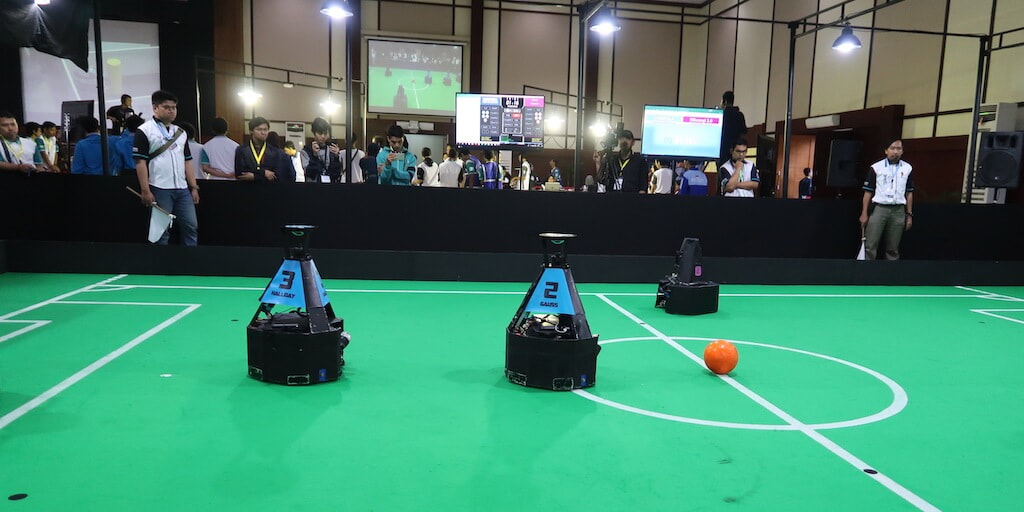
\includegraphics[width=0.8\textwidth]{resources/robotics-soccer.jpg}
    \caption{Tim DAGOZILLA pada Kontes Robot Indonesia}
    \label{fig:robotics-soccer}
    \bigskip
\end{figure}

Salah satu inisiatif untuk membangkitkan perkembangan di bidang robotika ini adalah liga pertandingan Robocup, yang merupakan liga pertandingan terbuka untuk tim pengembang dari universitas maupun organisasi lainnya untuk merekayasa robot-robot yang dapat ditandingkan antar tim. Diantara cabang liga yang ditandingkan dalam Robocup adalah kompetisi robot sepak bola beroda, dimana peserta mengembangkan tim robot-robot beroda yang harus berkoordinasi untuk mencetak gol di gawang lawan. Misi awal RoboCup saat didirikan adalah untuk mengumpulkan tim robot yang cukup maju untuk dapat mengalahkan tim manusia juara Piala Dunia pada tahun 2050. Inisiatif serupa juga ada di Indonesia dalam bentuk Kontes Robot Indonesia yang diselenggarakan oleh Kementerian Pendidikan dan Kebudayaan antar tim dari universitas-universitas Indonesia, seperti tim DAGOZILLA dari Institut Teknologi Bandung seperti pada gambar \ref{fig:robotics-soccer}.

Dalam rekayasa robotika, pembuatan modul persepsi yang akurat merupakan hal yang penting karena estimasi \textit{world state} atau keadaan dunia merupakan masukan robot untuk melakukan pengambilan keputusan dan aksi, sehingga kualitas estimasi yang buruk dapat mengakibatkan pengambilan keputusan yang salah dan membahayakan keamanan robot itu sendiri, pengguna, maupun orang lain yang mungkin terlibat. Dalam konteks robot sepak bola beroda, pelacakan pergerakan robot sendiri (yang disebut juga lokalisasi) maupun pergerakan objek lain yaitu robot teman, bola, maupun robot musuh merupakan informasi yang penting yang digunakan di banyak level dari pengambilan keputusan dan strategi tim sampai fungsionalitas dasar seperti mengejar, menggiring, mengoper, dan menembak bola.

Dalam kontes robot sepak bola, tidak terbacanya posisi suatu objek merupakan hal yang sering terjadi karena batasan jarak efektif sensor maupun halangan visual dari objek lain. Oleh karena itu, selain pengolahan data dari sensor yang dimiliki robot sendiri, pertukaran dan pengolahan data dari teman juga merupakan hal yang penting dalam persepsi \textit{world state} untuk mendapatkan estimasi yang selengkap dan seakurat mungkin.  Sayangnya, keterlambatan atau kegagalan penyampaian informasi antar robot anggota tim dapat terjadi karena inferensi jaringan, terutama di tempat kontes yang memiliki banyak penonton, sehingga algoritma pengolahan informasi harus didesain dengan baik untuk dapat tetap mengestimasi \textit{world state} dengan baik tanpa ataupun dengan menggunakan data yang terlambat dari teman.

Telah terdapat banyak penelitian mengenai cara penggabungan persepsi keadaan dari banyak robot di dalam maupun luar konteks robot sepak bola beroda, dan ada beberapa studi modifikasi algoritma estimasi sensor dengan masukan data yang mungkin terlambat, akan tetapi masih sedikit penelitian yang membahas dan menguji coba penggabungan persepsi keadaan dari banyak robot dalam konteks robot sepak bola beroda yang mempertimbangkan latensi di komunikasi.

Dalam tugas akhir ini, dikembangkan dan diuji coba modul estimasi persepsi \textit{world state} di lingkungan robot anggota tim untuk menangani kondisi komunikasi berlatensi pada konteks Kontes Robot Indonesia cabang sepak bola beroda.

\section{Rumusan Masalah}

Sesuai dengan latar belakang tersebut, masalah yang diselesaikan pada tugas akhir ini adalah mendesain, mengembangan, dan menguji coba algoritma estimasi persepsi \textit{world state} menggunakan pertukaran informasi banyak robot dengan latensi komunikasi, spesifik pada kasus pengembangan robot sepak bola beroda di Kontes Robot Indonesia. Untuk menyelesaikan permasalahan tersebut, masalah dibagi menjadi beberapa submasalah:

\begin{enumerate}
    \item Bagaimana memproses data dari sensor robot itu sendiri
    \item Bagaimana memproses informasi yang diterima dari teman yang mungkin terlambat karena latensi komunikasi
\end{enumerate}

\section{Tujuan}

Tujuan dari tugas akhir ini mengembangkan algoritma estimasi persepsi \textit{world state} dari robot anggota tim yang memberikan estimasi yang akurat, bahkan dalam keadaan kondisi jaringan komunikasi yang berlatensi. Berdasarkan dari submasalah yang ada, terdapat juga subtujuan:

\begin{enumerate}
    \item Mengembangkan algoritma pengolahan dan pelacakan data sensor robot sendiri yang akurat
    \item Mengembangkan algoritma integrasi informasi yang mungkin terlambat dari teman yang menghasilkan estimasi yang akurat
\end{enumerate}

\section{Batasan Masalah}

Batasan masalah yang diambil untuk membatasi lingkup penelitian di tugas akhir ini adalah:

\begin{enumerate}
    \item \textit{World state} yang diestimasi mencakup pergerakan posisi dan kecepatan robot anggota tim dan juga bola pada saat ini di lapangan.
    \item Eksperimen dilakukan dalam lingkungan simulasi yang dikembangkan sendiri sesuai dengan pemodelan mengikuti keadaan nyata dalam tim DAGOZILLA ITB dan Kontes Robot Indonesia.
    \item Algoritma yang dikembangkan tidak mencakup teknik dalam bidang \textit{Machine Learning} maupun \textit{Neural Network}.
\end{enumerate}

\section{Metodologi}

Pengerjaan tugas akhir dibagi menjadi beberapa tahapan:

\begin{enumerate}
    \item Pemodelan lingkungan nyata dan analisis solusi

          Pada tahap ini, dimodelkan lingkungan dunia nyata tempat robot bekerja, termasuk distribusi \textit{error} dari sensor dan distribusi latensi dari komunikasi. Dilakukan juga analisis masalah dan solusi untuk mendapatkan kerangka besar alur algoritma yang digunakan.

    \item Pembuatan lingkungan simulasi

          Pada tahap ini, dibuat lingkungan simulasi yang dapat disambungkan dengan lingkungan kode robot untuk melakukan pengujicobaan dengan profil \textit{error} dan latensi sesuai dengan pemodelan yang ada.

    \item Pengembangan algoritma solusi dan evaluasi

          Pada tahap ini, diimplementasi dan diuji coba algoritma-algoritma hipotesis solusi yang dicetuskan untuk dibandingkan berdasarkan hasil evaluasinya dalam lingkungan simulasi, untuk mendapatkan algoritma yang paling akurat.
\end{enumerate}

\section{Sistematika Pembahasan}

Selain Bab I Pendahuluan ini yang membahas mengenai latar belakang, rumusan masalah, dan metodologi, terdapat lima bab pada laporan tugas akhir ini dengan bahasannya masing-masing.

Bab II Studi Literatur membahas mengenai dasar teori yang didapatkan dari studi literatur yang digunakan untuk menyusun solusi dalam tugas akhir ini, baik dalam pemodelan dan pembuatan lingkungan simulasinya maupun solusi itu sendiri.

Bab III Analisis Solusi dan Arsitektur Sistem mendeskripsikan secara rinci masalah yang dihadapi, analisis dan desain solusi yang digunakan, juga rancangan umum arsitektur lingkungan simulasi tempat algoritma persepsi \textit{world state} berjalan.

Bab IV Eksperimen dan Analisis menjelaskan implementasi simulasi, eksperimen beserta hasil evaluasi dan analisisnya.

Bab V Penutup merangkum dan menyimpulkan hasil eksperimen dan analisis solusi yang diuji coba, beserta saran untuk penelitian lanjutan mengenai topik terkait persepsi \textit{world state} dalam keadaan latensi komunikasi.

\chapter{STUDI LITERATUR}

Bab ini memberikan pengetahuan prasyarat yang mendasari isi dari tugas akhir ini. Secara spesifik, bab ini membahas dasar teori probabilitas yang digunakan, aplikasinya dalam estimasi keadaan probabilistik, dan algoritma terkait; struktur dan cara kerja modul terkait pada perangkat lunak robot sepak bola tim Dagozilla; dan studi terkait yang sudah ada pada topik estimasi keadaan multiagen maupun estimasi keadaan dengan latensi data.

\section{Teori Probabilitas}

\subsection{Teorema Bayes}
Analog dengan definisi yang ada pada probabilitas kejadian, didefinisikan juga peluang kondisional
\begin{align}
    p(x \,|\, y) = Pr(X = x \,|\, Y = y) = \frac{p(x, y)}{p(y)}
\end{align}
yang digunakan untuk memodelkan peluang nilai $x$ terjadi apabila nilai $y$ terjadi. Dua variabel acak $X$ dan $Y$ disebut independen apabila untuk semua kemungkinan $x$ dan $y$ berlaku
\begin{align}
    p(x, y) = p(x) p(y) \quad\textit{atau}\quad p(x \,|\, y) = p(x)
\end{align}

Terkait peluang kondisional, Teorema Bayes menyatakan bahwa
\begin{align}
    p(x \,|\, y) = \frac{p(y \,|\, x)\, p(x)}{p(y)} = \eta\, p(y \,|\, x)\, p(x)
\end{align}
dimana $\eta = p(y)^{-1}$ merupakan suatu nilai yang konstan untuk semua kemungkinan $x$. Karena jumlah dari semua nilai $p(x \,|\, y)$ haruslah bernilai satu, $\eta$ disebut juga faktor normalisasi dan dapat ditentukan kemudian sebagai jumlah dari nilai $p(y \,|\, x)\, p(x)$ untuk semua kemungkinan $x$.

Teorema Bayes sangat berguna untuk memperbarui kepercayaan terhadap distribusi peluang $x$ setelah mengetahui terjadinya $y$ apabila diketahui peluang terjadinya $y$ dapat ditentukan untuk setiap kemungkinan $x$.

\subsection{Distribusi Gaussian}

Salah satu distribusi yang penting dan banyak dipelajari adalah keluarga distribusi Gaussian atau distribusi normal dimana dengan nilai rata-rata $\mu$ dan nilai variansi $\sigma^2$ memiliki fungsi densitas
\begin{align}
    p(x) = \frac{1}{\sigma \sqrt{2\pi}} \exp\left\{-\frac{1}{2}\left(\frac{x-\mu}{\sigma}\right)^2\right\}
\end{align}
dengan kasus spesial dimana $\mu = 0$ dan $\sigma^2 = 1$ disebut juga distribusi normal standar.

Distribusi Gaussian banyak dipelajari karena beberapa alasan. Salah satu alasan adalah karena distribusi ini memiliki banyak properti yang membuatnya mudah dimanipulasi dan digunakan, diantaranya adalah fungsi distribusi penjumlahan variabel-variabel acak independen berdistribusi Gaussian, maupun perkalian dan konvolusi fungsi Gaussian juga merupakan fungsi Gaussian. Alasan lainnya adalah diobservasi juga berbagai variabel acak di berbagai pengujian ilmiah yang ternyata memiliki distribusi yang hampir mirip dengan Gaussian. Selain itu juga, terbukti bahwa berdasarkan Teorema Limit Pusat, rata-rata dari banyak variabel acak distribusi identik independen akan mendekati distribusi Gaussian. \citep{degroot2012}

Disebabkan oleh alasan-alasan tersebut, praktisnya distibusi Gaussian banyak digunakan untuk memodelkan berbagai variabel acak di dunia nyata, seperti distribusi sampel dari populasi yang sangat besar maupun distribusi error pada suatu pengukuran atau kontrol sering diasumsikan memiliki distribusi Gaussian.

Distribusi Gaussian memiliki generalisasi ke dalam vektor acak yaitu kumpulan variabel acak yang direpresentasikan dalam bentuk vektor. Dengan parameter vektor rata-rata $\mu$ dan matriks kovarian $\Sigma$ yang bersifat simetrik dan positif semidefinit, didefinisikan fungsi densitas
\begin{align}
    p(x) = det(2 \pi \Sigma)^{-\frac{1}{2}} \exp\left\{-\frac{1}{2}(x-\mu)^T \Sigma^{-1} (x-\mu)\right\}
\end{align}
dimana masing-masing komponen $X_i$ sendiri memiliki distribusi Gaussian dengan rata-rata $\mu_i$ dan kovarian antara $X_i, X_j$ sama dengan $\Sigma_{i,j}$.

\section{Estimasi Keadaan Probabilistik}

Perangkat lunak di robot atau sistem lainnya yang membaca \textit{world state} nyata menggunakan sensor, dan mungkin berinteraksi dengannya menggunakan aktuator, mempunyai kebutuhan untuk menentukan keadaan tersebut dari bacaan sensor. Secara umum, digunakan model matematika yang bertujuan untuk mentranslasi data pengukuran menjadi model \textit{world state}. Seiring berjalannya waktu, penggunaan estimasi \textit{world state} menggunakan model probabilistik menjadi lebih populer dibandingkan model perhitungan yang deterministik. Dengan memodelkan \textit{world state} yang diketahui menjadi suatu distribusi peluang, hasil pengukuran \textit{world state} menjadi lebih tahan terhadap efek error pada data pengukuran. \citep{thrun2010}

\subsection{Pemodelan Keadaan}

Dalam model probabilistik, \textit{world state} disimbolkan sebagai suatu vektor acak $X$, dimana $x_t$ menandakan \textit{world state} pada waktu ke-$t$. Vektor acak ini mengandung berbagai variabel acak misalnya posisi dan orientasi sesungguhnya dari robot maupun objek lain pada suatu waktu.

Sistem melakukan pengukuran terhadap dunia yang disimbolkan sebagai vektor acak $Z$ dan instansiasinya $z_t$ yang merupakan pengukuran dari dunia nyata pada waktu ke-$t$. Sedangkan apabila sistem melakukan interaksi umpan balik terhadap dunia nyata menggunakan suatu aktuator yang dikontrol oleh sistem, maka perintah interaksi tersebut disimbolkan sebagai vektor acak $U$ dan $u_t$ yang merupakan kontrol interaksi saat sistem sedang melakukan transisi dari $x_{t-1}$ ke $x_t$.

Perhatian dari estimasi keadaan probabilistik adalah mengestimasi nilai dari $x_t$ diberikan nilai $z$ dan $u$ yang terjadi sebelumnya. Dalam persamaan matematika, hendak dihitung
\begin{align}
    bel(x_t) = p(x_t \,|\, z_{1:t}, u_{1:t}) \,,
\end{align}
atau distribusi peluang alternatif dimana diprediksi nilai dari $x_t$ sebelum mendapat hasil pengukurannya $z_t$,
\begin{align}
    \overline{bel}(x_t) = p(x_t \,|\, z_{1:t-1}, u_{1:t}) \,.
\end{align}

Mengasumsikan nilai $X$ mengandung semua \textit{world state} yang relevan terhadap sistem pada waktu sekarang, maka tidak ada informasi tambahan yang bisa diberikan oleh pengukuran $z_t$ maupun keadaan sebelumnya $x_{t-k}$ terhadap keadaan berikutnya $x_{t+1}$ di luar apa yang terkandung pada $x_t$. Oleh karena itu dalam pembangkitan nilai $x_t$ dan $z_t$, dua distribusi peluang yang penting diperhatikan adalah peluang transisi keadaan
\begin{align}
    p(x_t \,|\, x_{0:t-1}, z_{1:t-1}, u_{1:t}) = p(x_t \,|\, x_{t-1}, u_t)
\end{align}
dan peluang pengukuran
\begin{align}
    p(z_t \,|\, x_{0:t}, z_{1:t-1}, u_{1:t}) = p(z_t \,|\, x_t)
\end{align}

\begin{figure}[h]
    \centering
    \includegraphics[width=0.8\textwidth]{resources/hidden-markov-model.png}
    \caption{Hubungan $X, U, Z$}
    \label{fig:hidden-markov-model}
\end{figure}

Hubungan ini digambarkan pada gambar \ref{fig:hidden-markov-model}. Peluang yang hanya saling berpengaruh antar tahapan waktu yang berdekatan disebut juga \textit{hidden Markov model} atau \textit{dynamic Bayes network}.

\subsection{Penapis Bayes}

\begin{algorithm}
    \caption{Penapis Bayes}
    \label{alg:bayes-filter}
    \begin{algorithmic}[1]
        \Function{bayes\_filter}{$bel(x_{t-1}), u_t, z_t$}
        \ForAll{$x_t$}
        \State $\overline{bel}(x_t) = \int p(x_t \,|\, u_t, x_{t-1})\, bel(x_{t-1})\, dx_{t-1}$
        \State $bel(x_t) = \eta\, p(z_t \,|\, x_t)\, \overline{bel}(x_t)$ \Comment{$\eta$ menormalisasi nilai dari $bel(x_t)$}
        \EndFor
        \State \Return $bel(x_t)$
        \EndFunction
    \end{algorithmic}
\end{algorithm}

Perhatikan bahwa perubahan nilai dari $\overline{bel}(x_{t-1})$ ke $bel(x_t)$ dapat ditentukan dari peluang transisi keadaan $p(x_t \,|\, x_{t-1}, u_t)$, dan perubahan nilai dari $bel(x_t)$ ke $\overline{bel}(x_t)$ dapat ditentukan dari peluang pengukuran $p(z_t \,|\, x_t)$ menggunakan Teorema Bayes. Memanfaatkan fakta tersebut, dirumuskan algoritma penapis Bayes atau \textit{Bayes filter algorithm} pada algoritma \ref{alg:bayes-filter}. Baris tiga menunjukkan perhitungan nilai $bel(x_t)$ sebagai ekspansi dari penjumlahan nilai $p(x_t, x_{t-1})$ saat diketahui $u_t$ untuk semua kemungkinan $x_{t-1}$, spesifik untuk kasus kontinu. Tahap ini sering disebut tahap prediksi. Baris empat memanfaatkan teorema Bayes untuk mendapatkan distribusi $x_t$ setelah mendapatkan informasi dari $z_t$. Tahap ini sering disebut tahap pembaruan pengukuran.

Algoritma penapis digunakan untuk mengiterasi nilai dari $bel(x_t)$ seiring waktu, dan merupakan algoritma yang optimal mengasumsikan proses merupakan \textit{hidden Markov model}. Perhatikan bahwa algoritma ini mengharuskan pemodelan sendiri nilai dari peluang transisi keadaan, peluang pengukuran, dan distribusi awal $bel(x_0)$ yang akan digunakan.

Selain itu, karena nilai dari $bel(x_t)$ merupakan distribusi peluang, dalam aplikasinya dibutuhkan pendekatan untuk memodelkan distribusi tersebut sehingga dapat dikomputasi oleh komputer. Pada praktisnya, distribusi peluang $bel(x_t)$ dimodelkan sebagai distribusi dengan jenis yang dapat diparameterasikan seperti pada penapis Kalman, atau distribusi tersebut didiskritkan seperti pada penapis histogram atau penapis partikel.

\subsection{Penapis Kalman}

Pada penapis Kalman atau \textit{Kalman Filter} (\textit{KF}), distribusi dari $bel(x_t)$ dan $\overline{bel}(x_t)$ diasumsikan memiliki distribusi Gaussian dengan parameter $\mu$ dan $\sigma^2$ yang dicari pada setiap iterasi algoritmanya. Agar penapis Bayes Gaussian bekerja, distribusi peluang transisi keadaan dan peluang pengukuran harus memiliki restriksi tambahan.

Pada variasi penapis Kalman yang paling sederhana, direstriksi bahwa (1) vektor acak $x_t$ merupakan kombinasi linear dari $x_{t-1}, u_t,$ dan faktor error $\epsilon_t$
\begin{align}
    x_t = A_t x_{t-1} + B_t u_t + \epsilon_t \,
\end{align}
untuk $x_t$ berdimensi $n$, $u_t$ berdimensi $m$, $A_t$ matriks berdimensi $n \times n$, dan $B_t$ berdimensi $n \times m$, dan $\epsilon_t$ vektor acak Gaussian dengan rata-rata nol dan kovariansi $R_t$; (2) $z_t$ merupakan kombinasi linear dari $x_t$ dan faktor error $\delta_t$
\begin{align}
    z_t = C_t x_t + \delta_t
\end{align}
untuk $z_t$ berdimensi $k$, $C_t$ berdimensi $k \times n$, dan $\delta_t$ vektor acak Gaussian dengan rata-rata nol dan kovariansi $Q_t$; dan (3) distribusi awal $bel(x_0)$ memiliki distribusi Gaussian. Ketiga asumsi ini menjamin bahwa distribusi $bel(x_t)$ merupakan distribusi Gaussian untuk semua waktu $t$ yang akan datang.

\begin{algorithm}
    \caption{Penapis Kalman}
    \label{alg:kalman-filter}
    \begin{algorithmic}[1]
        \Function{kalman\_filter}{$\mu_{t-1}, \Sigma_{t-1}, u_t, z_t$}
        \State $\overline{\mu}_t = A_t\, \mu_{t-1} + B_t\, u_t$
        \State $\overline{\Sigma}_t = A_t\, \Sigma_{t-1}\, A_t^T + R_t$
        \State $K_t = \overline{\Sigma}_t\, C_t^T\, (C_t\, \overline{\Sigma}_t\, C_t^T + Q_t)^{-1}$
        \State $\mu_t = \overline{\mu}_t + K_t(z_t - C_t\, \overline{\mu}_t)$
        \State $\Sigma_t = (I - K_t\, C_t)\, \overline{\Sigma}_t$
        \State \Return $\mu_t, \Sigma_t$
        \EndFunction
    \end{algorithmic}
\end{algorithm}

Berdasarkan hubungan di atas, algoritma penapis Kalman menghitung nilai dari parameter rata-rata $\mu_t$ dan kovariansi $\Sigma_t$ dari distribusi Gaussian $bel(x_t)$. Sehingga dapat diturunkan algoritma penapis Kalman seperti pada algoritma \ref{alg:kalman-filter}.

Disebabkan restriksi linearitas pada peluang transisi keadaan dan peluang pengukuran, algoritma penapis Kalman tidak dapat digunakan apabila restriksi linearitas tersebut tidak dipenuhi. Agar penapis Kalman dapat digunakan untuk kasus $x_t = g(u_t, x_{t-1}) + \epsilon_t$ dan $z_t = h(x_t) + \sigma_t$ dimana fungsi $g$ dan $h$ tidak linear, fungsi tersebut harus diaproksimasi terlebih dahulu agar menjadi linear.

Pada \textit{Extended Kalman Filter}, fungsi dilinearkan menggunakan turunan parsial dari fungsi $g$ dan $h$. Dengan menghitung $G_t = g'(u_t, \mu_{t-1})$ dan $H_t = h'(\overline{\mu}_t)$ dimana $g'$ merupakan turunan parsial $g$ terhadap $x_{t-1}$, didapatkan persamaan linear
\begin{align}
    g(u_t, x_{t-1}) \approx g(u_t, \mu_{t-1}) + G_t\, (x_{t-1} - \mu_{t-1}) \\
    h(x_t) \approx h(\overline{\mu}_t) + H_t\, (x_t - \overline{\mu}_t)
\end{align}
Nilai $A$ dan $C$ pada penapis Kalman dapat digantikan dengan nilai $G$ dan $H$.

Pada \textit{Unscented Kalman Filter}, fungsi dilinearkan dengan mengambil sampel nilai pada fungsi $g$ dan $h$, lalu membuat persamaan linear dengan melakukan regresi pada nilai masukan secara umum. Sampel diambil di rata-rata $\mu$ dan dua titik di sekelilingnya untuk setiap dimensi yang ada.

\subsection{Penapis Histogram}

\begin{algorithm}
    \caption{Penapis Bayes Diskrit}
    \label{alg:discrete-bayes-filter}
    \begin{algorithmic}[1]
        \Function{discrete\_bayes\_filter}{$\{p_{k, t-1}\}, u_t, z_t$}
        \ForAll{$k$}
        \State $\overline{p}_{k, t} = \sum_i p(X_t = x_k \,|\, u_t, X_{t-1} = x_i)\, p_{i, t-1}$
        \State $p_{k, t} = \eta\, p(z_t \,|\, X_t = x_k)\, \overline{p}_{k, t}$ \Comment{dinormalisasi untuk semua $k$}
        \EndFor
        \State \Return $\{p_{k, t}\}$
        \EndFunction
    \end{algorithmic}
\end{algorithm}

Pada penapis histogram, kemungkinan nilai dari $x_t$ terbatas dan dibagi-bagi menjadi sebanyak terbatas daerah, misalnya kemungkinan posisi dari robot pada lapangan berdimensi $9 \times 6$ meter persegi dapat dibagi menjadi $1350$ daerah berbentuk persegi berukuran $20 \times 20$ sentimeter persegi dalam suatu grid. Pada algoritma ini, $bel(x_t)$ direpresentasikan sebagai suatu tabel yang menyimpan peluang nilai berada dalam masing-masing daerah yang ada. Algoritma ini pun relatif lebih sederhana karena hanya perlu mendiskritkan perhitungan pada filter Bayes.

Algoritma filter Bayes diskrit ada di algoritma \ref{alg:discrete-bayes-filter}. Apabila fungsi peluang transisi keadaan atau peluang pengukuran yang dimiliki bersifat kontinu, dapat diaproksimasi menjadi diskrit seperti
\begin{align}
    p(\mathbf{x}_{k, t} \,|\, u_t, \mathbf{x}_{i, t-1}) \approx |\mathbf{x}_{k, t}|\, p(\hat{x}_{k, t} \,|\, u_t, \hat{x}_{i, t-1}) \\
    p(z_t \,|\, \mathbf{x}_{k, t}) \approx p(z_t \,|\, \hat{x}_{k, t})
\end{align}
dimana $\hat{x}_{k, t}$ adalah representasi dari daerah $\mathbf{x}_{k, t}$ seperti titik tengahnya, dan $|\mathbf{x}_{k, t}|$ adalah luas daerahnya

Teknik histogram ini berkaitan erat dengan grid okupansi dimana masing-masing daerah di grid tersebut diisi dengan tingkat kepercayaan suatu nilai berada dalam daerah tersebut, walau berbeda dengan histogram peluang dimana jumlah dari nilai semua grid haruslah bernilai satu. Aplikasi dari teknik ini dalam permasalahan lokalisasi robot kerap disebut dengan \textit{Markov localization}.

\subsection{Penapis Partikel}

Pada penapis partikel, distribusi peluang nilai dari $bel(x_t)$ direpresentasikan dengan menyimpan koleksi sejumlah nilai $x_t$ atau disebut sebagai partikel, dimana distribusi dari partikel tersebut mengaproksimasi distribusi dari $bel(x_t)$ yang sesungguhnya. Semakin banyak partikel yang disimpan, semakin akurat algoritma penapis partikel ini, tetapi semakin besar juga sumber daya memori dan waktu yang dibutuhkan.

\begin{algorithm}
    \caption{Penapis Partikel}
    \label{alg:particle-filter}
    \begin{algorithmic}[1]
        \Function{particle\_filter}{$\chi_{t-1}, u_t, z_t$}
        \State $\overline{\chi}_t= \overline{\chi}_t = \emptyset$
        \For{$m = 1$ to $M$}
        \State sample $x_t^{[m]} \sim p(x_t \,|\, u_t, x_{t-1}^{[m]})$
        \State $w_t^{[m]} = p(z_t \,|\, x_t^{[m]})$
        \State add $(x_t^{[m]}, w_t^{[m]})$ to $\overline{\chi}_t$
        \EndFor
        \For{$m = 1$ to $M$}
        \State draw $i$ with probability $\propto w_t^{[i]}$
        \State add $x_t^{[i]}$ to $\chi_t$
        \EndFor
        \State \Return $\chi_t$
        \EndFunction
    \end{algorithmic}
\end{algorithm}

Algoritma penapis partikel digambarkan di algoritma \ref{alg:particle-filter}. Baris empat merupakan tahap prediksi dimana untuk setiap partikel sebelumnya dibangkitkan partikel sekarang menggunakan nilai kontrol. Partikel tersebut disimpan di himpunan $\overline{\chi}_t$ beserta evaluasi peluangnya berdasarkan pengukuran. Agar suatu partikel dengan peluang yang lebih besar memiliki lebih banyak representasi dalam himpunan $\chi_t$, dilakukan sampling ulang terhadap $x_t$ dengan peluang sebanding dengan hasil evaluasinya, pada baris delapan sampai sebelas.

Secara umum, penapis partikel ini merupakan pilihan paling populer dalam melakukan estimasi terhadap keadaan nonGaussian, karena komputasinya yang mengandalkan sampling relatif lebih mudah dan tingkat akurasi terhadap performa algoritma dapat diatur dengan mudah melalui banyak partikel yang digunakan. Ada beberapa kondisi yang mengakibatkan ketidakakuratan pada algoritma ini, seperti saat terjadi konvergensi partikel di nilai yang salah, sehingga peningkatan pada algoritma ini diantaranya adalah dengan menambahkan faktor error tambahan pada tahap prediksi dan/atau memasukkan partikel baru di luar $\overline{\chi}_t$ ke dalam $\chi_t$.

Penggunaan populer dari algoritma ini adalah pada algoritma \textit{Monte Carlo localization} (\textit{MCL}) dimana penapis partikel digunakan untuk kasus lokalisasi robot menggunakan data kontrol dari kontrol kecepatan atau data perpindahan dari sensor dan data pengukuran dari sensor peraba jarak atau kamera. Algoritma \textit{Augmented Monte Carlo localization} (\textit{AMCL}) merupakan modifikasi algoritma \textit{MCL} biasa yang ditambahkan pemasukkan partikel baru apabila hasil evaluasi partikel-partikel yang ada sekarang lebih buruk dari sebelumnya.

\section{Studi Terkait}

Secara umum, teknik probabilistik seperti penapis Kalman maupun penapis partikel telah banyak diimplementasi dalam kasus pelacakan objek oleh satu agen dan telah menunjukkan tingkat keberhasilan yang cukup baik. Sedangkan dalam kasus pelacakan objek oleh banyak agen, terdapat banyak studi yang mencetuskan beragam ide yang sangat bervariasi dalam berbagai konteks. Dalam konteks kontes robot sepak bola sendiri, sudah terdapat beberapa studi yang mencoba menggabungkan data pelacakan objek maupun lokalisasi.

Robot-robot \citet{stroupe2001} melacak posisi bola menggunakan penapis Kalman dan distribusi hasilnya disebarkan ke robot lainnya, dimana distribusi Gaussian dari semua robot akan digabungkan oleh masing-masing robot untuk menghasilkan suatu distribusi Gaussian akhir. Asumsi dasar dari makalah ini adalah \textit{error}nya bersifat normal independen, lokalisasi robot sempurna, dan waktu pengukuran bersamaan. Sedangkan \citet{pinheiro2004} mengalikan langsung distribusi Gaussian masing-masing robot untuk mendapatkan fungsi objektif lokasi bola. Data digabungkan apabila hasil perkalian memiliki puncak probabilitas yang unik, dimana dibuat suatu rumus untuk menentukan apakah ini terjadi.

\citet{ferrein2005} membandingkan beberapa metode untuk menggabungkan observasi bola dari masing-masing robot, seperti merata-ratakan posisi pengamatan, menggunakan penapis Kalman menggunakan terhadap posisi bola menggunakan data yang didapat masing-masing robot, menggunakan penapis partikel, maupun menggunakan penapis histogram yang digabungkan ke estimasi global menggunakan penapis Kalman. Hasilnya adalah penapis Kalman sederhana memiliki tingkat akurasi dan kecepatan yang paling baik.

Masing-masing robot \citet{pahliani2006} melakukan lokalisasi menggunakan \textit{Markov localization}, lalu tergantung dari posisi robot, robot-robot yang ada membentuk beberapa kelompok kecil untuk bertukar informasi. Data dari robot di kelompok yang sama dibagikan, lalu menggunakan data yang didapat dari kelompok lain, hasil lokalisasi dari masing-masing robot diperbaiki secara Bayes. Setelah lokalisasi, deteksi objek juga dilakukan menggunakan alur dan kelompok yang sama.

\citet{santos2009} melacak bola menggunakan penapis partikel. Untuk mengefisiensikan pertukaran informasi antar robot, distribusi dalam bentuk partikel diubah dulu menjadi \textit{gaussian mixture model} yang terdiri dari beberapa distribusi Gauss menggunakan algoritma \textit{expectation maximization} yang bekerja mirip seperti algoritma \textit{K means}. Ada juga ukuran persetujuan informasi antar robot menggunakan \textit{covariance intersection} untuk menentukan apakah informasi baru diintegrasi dengan informasi robot sendiri atau tidak. \citet{ahmad2011} mengembangkan ide ini dengan membuat algoritma penggabungan distribusi dari masing-masing robot dimana dibangkitkan kumpulan partikel baru dengan melakukan \textit{sampling} dari distribusi-distribusi yang ada berdasarkan tingkat kepercayaan distribusi tersebut sebagai masukan dari penapis partikel.

\citet{ahmad2013} mengumpulkan semua pengukuran posisi relatif semua robot terhadap robot lain, objek statis, maupun objek dinamis, dan mencari konfigurasi posisi semua objek yang meminimasi \textit{error} dari pengukuran-pengukuran yang ada menggunakan \textit{iterative local linearization} atau \textit{least square minimization}. Kelebihan teknik ini diantara adalah beban komputasinya linear terhadap banyak robot, akan tetapi setiap robot harus menunggu sampainya data pengukuran dari semua robot lain.

\citet{chang2016} menggunakan \textit{Extended Kalman Filter} untuk melacak sistem seluruh robot dan objek. \textit{Update} dilakukan untuk masing-masing robot, sedangkan pengukuran diintegrasi berdasarkan robot apa saja yang terlibat dalam pengukuran tersebut. Teknik \textit{multiple hypothesis tracking} digunakan untuk mengasosiasikan data pengukuran dengan posisi objek di hipotesis.

\citet{ahmad2017} menggunakan penapis partikel yang mencakup posisi semua robot ditambah objek yang diobservasi. Masing-masing bagian partikel dari robot digerakan dan dievaluasi secara terpisah, dan diurutkan ulang sehingga bagian partikel dengan evaluasi tinggi dari suatu robot dipasangkan dengan bagian partikel robot lain dengan evaluasi yang tinggi juga. Algoritma ini lalu memasangkan partikel bagian dari objek yang memaksimalkan evaluasi partikel bagian tersebut dengan partikel bagian robot dengan evaluasi tinggi juga. Teknik ini menyelesaikan masalah defisiensi partikel pada penapis partikel tanpa harus menambahkan banyak partikel secara eksponensial.


\chapter{ANALISIS SOLUSI DAN ARSITEKTUR SISTEM}

Bab ini menjelaskan mengenai arsitektur lingkungan simulasi sebagai tempat uji coba, detail analisis masalah, desain arsitektur solusi, dan desain algoritma estimasi yang dapat digunakan.

\section{Arsitektur Lingkungan Simulasi}

\begin{figure}[h]
    \centering
    \medskip
    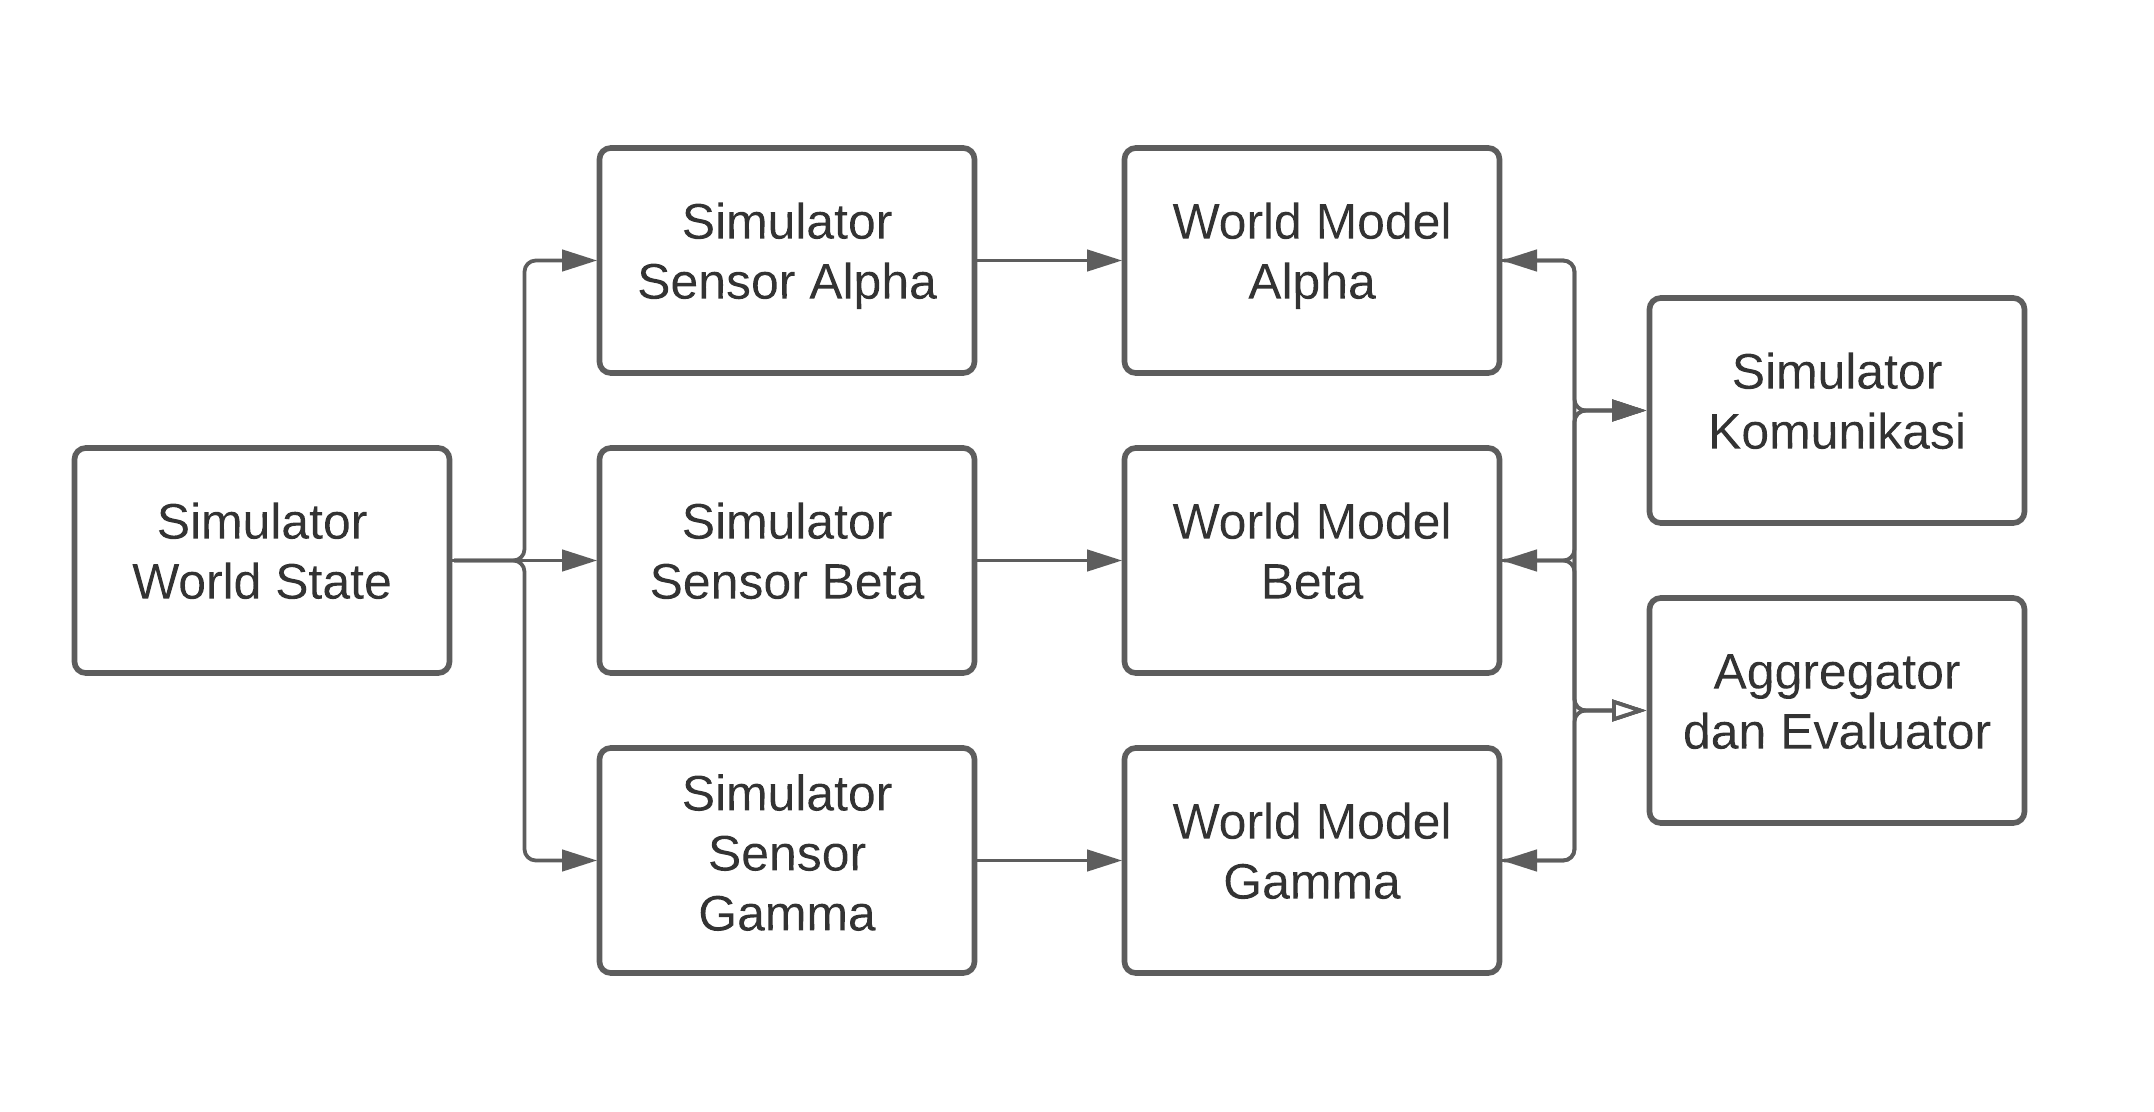
\includegraphics[width=0.8\textwidth]{resources/simulation-structure.png}
    \caption{Struktur modul simulasi}
    \label{fig:simulation-structure}
    \bigskip
\end{figure}

Lingkungan simulasi dikembangan dalam \textit{framework} ROS, dimana arsitektur lingkungan simulasi digambarkan di \ref{fig:simulation-structure} dimana masing-masing \textit{node} berjalan dengan periode komputasi $30$ ms yang didasari pada periode ketersediaan data sensor di keadaan nyata. Selain \textit{node} \textit{world model} yang bertugas untuk menampung algoritma estimasi \textit{world state}, terdapat beberapa \textit{node} simulator yang bertujuan untuk membangkitkan data pengujian untuk menganalisis akurasi algoritma estimasi.

\subsection{Simulator \textit{World State}}

\begin{figure}[h]
    \centering
    \medskip
    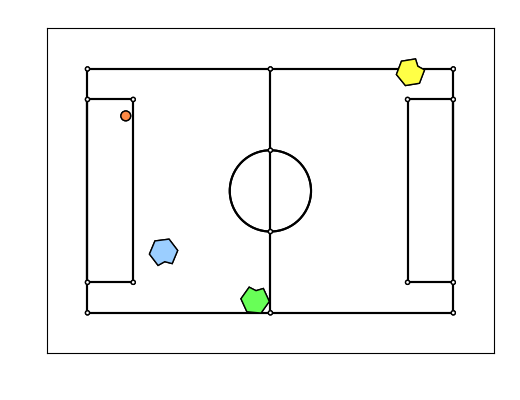
\includegraphics[width=0.8\textwidth]{resources/true-world-state.png}
    \caption{Keadaan \textit{world state} sesungguhnya}
    \label{fig:true-world-state}
    \bigskip
\end{figure}

Modul simulator \textit{world state} seperti pada \ref{fig:true-world-state} bertujuan untuk membangkitkan nilai \textit{world state} uji coba yang sebenarnya, yang mencakup pergerakan dari masing-masing robot tim dan bola. Simulasi dilakukan di lapangan $9 \times 6$ meter kuadrat sesuai spesifikasi pertandingan regional Kontes Robot Indonesia cabang sepak bola beroda tahun 2019. Terdapat dinding dengan jarak satu meter di sekitar lapangan untuk mencegah robot dan terutama bola untuk keluar dari lapangan. Tiga robot tim yang disimulasikan, bernama alpha, beta, dan gamma, digerakan oleh suatu perencana gerakan sementara yang sekali-kali membangkitkan target \textit{pose} yang harus dituju oleh robot terkait. Masing-masing robot lalu mendekati target \textit{pose} masing-masing dengan gerakan lurus sekaligus dengan rotasi dengan kecepatan maksimum $2$ meter per detik dan akselerasi maksimum $1.5$ meter per detik kuadrat. Pergerakan bola dibangkitkan dengan terus meng\textit{update} kecepatan bola setiap periode komputasi dengan perubahan kecepatan di sumbu x dan y mengikuti distribusi normal dengan variansi sebesar $0.16$ meter per detik dikuadratkan dikali periode komputasi, dan kecepatan maksimal $2$ meter per detik. Simulator \textit{world state} juga mengecek apakah terjadi tabrakan antar robot, bola, ataupun dinding, dimana bola akan memantul sedangkan robot akan berhenti dan menghasilkan target \textit{pose} baru untuk keluar dari tabrakan.

\subsection{Simulator Sensor}

\begin{figure}[h]
    \centering
    \medskip
    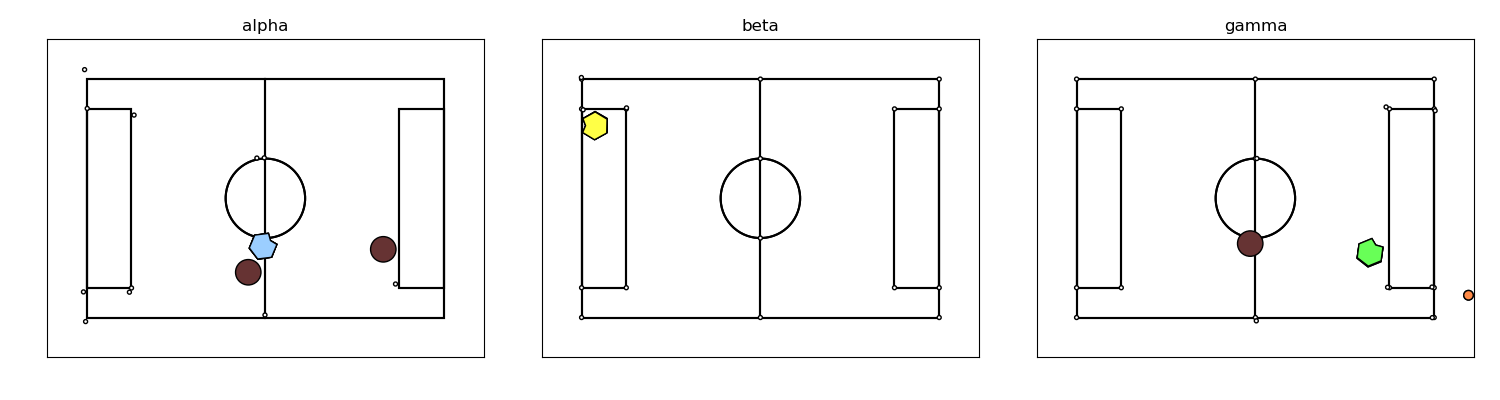
\includegraphics[width=\textwidth]{resources/allies-sensor.png}
    \caption{Bacaan sensor masing-masing robot}
    \label{fig:allies-sensor}
    \bigskip
\end{figure}

Terdapat tiga \textit{node} simulator sensor untuk masing-masing robot yang mengikuti pesan \textit{world state} dari \textit{node} simulator \textit{world state} dan menghitung hasil bacaan sensor dari robot tersebut, yang mencakup simulasi bacaan odometri berupa perpindahan \textit{pose} dari robot terhadap \textit{pose} di periode komputasi sebelumnya; simulasi bacaan kompas berupa orientasi absolut dari robot; dan simulasi persepsi \textit{vision} dari kamera yang mencakup posisi relatif dari \textit{landmark}, bola apabila terlihat, dan teman yang terlihat. \textit{Landmark} merupakan $16$ titik-titik statis yang tersebar di sekitar lapangan yang dapat dilihat oleh robot untuk membantu proses lokalisasi dari robot tersebut. Persepsi \textit{vision} terbatas dalam suatu rentang penglihatan robot sebesar radius maksimal $4$ meter yang juga terpengaruh oleh oklusi terhalangnya suatu objek oleh objek lain, seperti robot teman menghalangi persepsi bola atau \textit{landmark} dibelakangnya, atau suatu peluang kecil dimana suatu objek yang harusnya terlihat gagal dideteksi oleh \textit{vision} seperti pada \ref{fig:allies-sensor}. \textit{Vision} tidak dapat membedakan antara satu \textit{landmark} dengan \textit{landmark} lainnya ataupun satu teman dengan lainnya.

Masing-masing bacaan ditambahkan \textit{error} dengan variansi yang proporsional terhadap bacaan sesungguhnya. Bacaan odometri memiliki \textit{error} dengan variansi sebesar jarak perpindahan sebenarnya dikali sekitar $0,02$. Sedangkan bacaan \textit{vision} memiliki \textit{error} dengan variansi sebesar jarak objek sebenarnya dikali $0,0036$ untuk \textit{error} sejajar dengan arah objek dan $0,0009$ untuk \textit{error} tegak lurus arah objek.

\subsection{Simulator Komunikasi}

\begin{figure}[h]
    \centering
    \medskip
    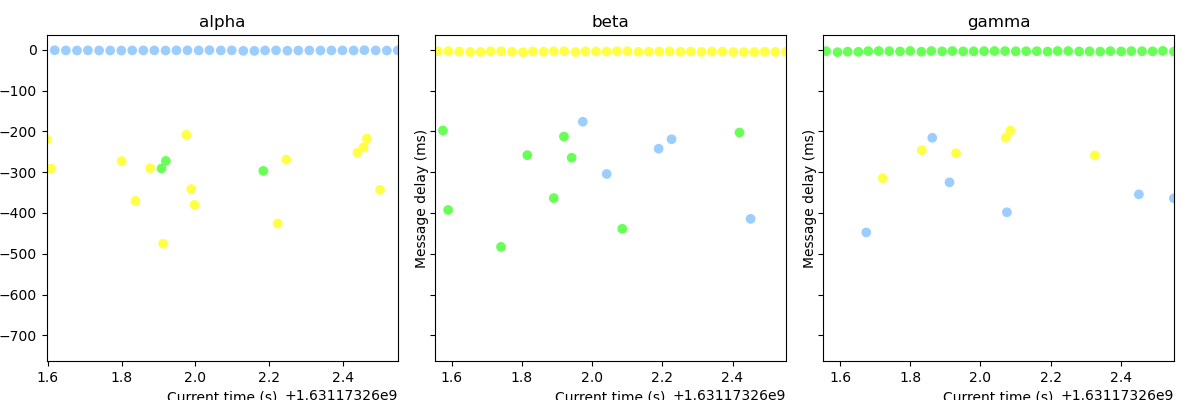
\includegraphics[width=\textwidth]{resources/allies-comm.png}
    \caption{Latensi komunikasi}
    \label{fig:allies-comm}
    \bigskip
\end{figure}

\textit{Node} \textit{world model} dapat menyiarkan pesan ke temannya, yang akan diterima oleh \textit{node} simulator komunikasi dan disiarkan balik ke semua temannya setelah suatu latensi komunikasi dan peluang hilangnya pesan. Simulator komunikasi dimodelkan dengan hidden Markov model dengan dua \textit{state}, yang menandakan kondisi jaringan baik dengan latensi komunikasi berdistribusi \textit{shifted gamma} dengan rata-rata $35$ ms, minimum $20$ ms, standar deviasi $10$ ms, dan kemungkinan hilangnya pesan sebesar $5\%$; dan kondisi jaringan buruk dengan latensi dengan rata-rata $300$ ms, minimum $150$ ms, standar deviasi $100$ ms, dan kemungkinan hilangnya pesan sebesar $65\%$.

\subsection{Aggregator dan Evaluator}

\begin{figure}[h]
    \centering
    \medskip
    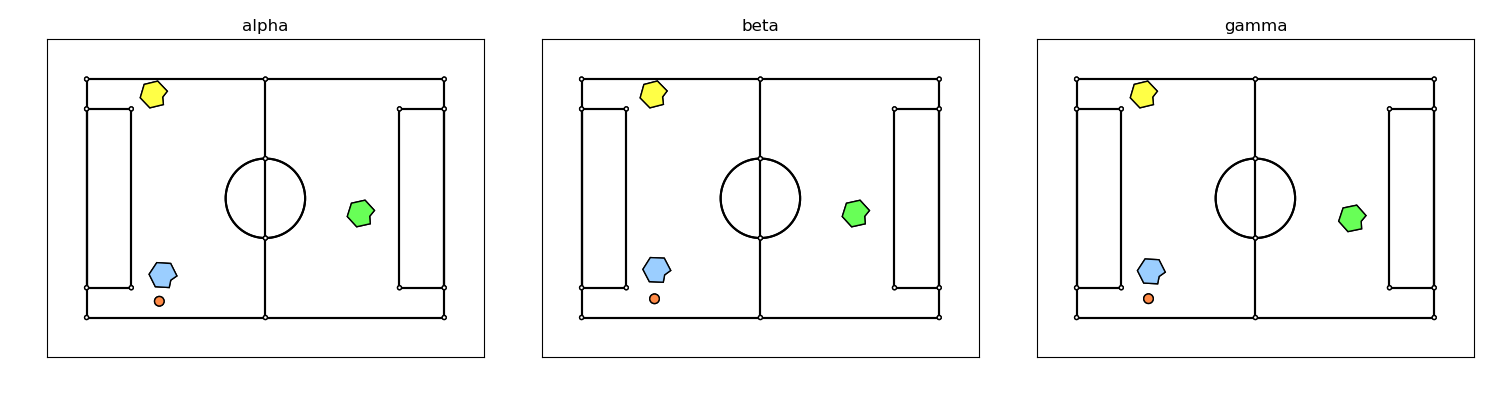
\includegraphics[width=\textwidth]{resources/allies-world-model.png}
    \caption{Estimasi \textit{world state} masing-masing robot}
    \label{fig:allies-world-model}
    \bigskip
\end{figure}

\textit{Node-node} aggregator dan evaluator mengikuti hasil estimasi dari \textit{world model} yang ada dan nilai sebenarnya dari \textit{world state} untuk melakukan evaluasi kinerja algoritma dan hal lain seperti visualisasi seperti pada \ref{fig:allies-world-model}. Evaluasi performa dari suatu algoritma diambil dari metrik \textit{error} berupa jarak hasil estimasi dan keadaan sebenarnya dari masing-masing objek dimana nilai $I/M$ dari robot bernilai $0.4$.

\section{Analisis Studi Terdahulu}

Dari studi yang sudah diteliti, didapat bahwa walaupun sudah cukup banyak studi yang membahas mengenai algoritma estimasi \textit{world model} yang melacak posisi robot maupun bola di kontes robot sepak bola, hampir semua studi tersebut mengasumsikan bahwa komunikasi antar robot memiliki latensi yang dapat diabaikan. Studi yang melakukan pengujian pada kasus kegagalan komunikasi berjumlah sedikit dan juga hanya menguji kasus kegagalan komunikasi total pada suatu robot. Banyak algoritma yang dibahas dari studi sebelumnya tidak dapat bekerja secara efektif dalam keadaan latensi komunikasi yang signifikan, seperti teknik merata-ratakan data, menggabungkan distribusi Gaussian data, maupun melakukan minimasi \textit{error} terhadap sistem. Algoritma \citet{ahmad2017} dibahas sebagai algoritma yang bersifat \textit{online} yang tidak membutuhkan terkumpulnya informasi dari robot-robot lainnya sebelum suatu robot dapat mulai melakukan kalkulasi estimasi, tetapi studi tersebut tetap tidak menangani integrasi data yang terlambat dan di luar urutan.

Secara umum, di luar konteks kontes robot sepak bola beroda, walau terdapat banyak studi yang membahas penggabungan data dari banyak sensor dengan latensi dan keterlambatan, masih sedikit studi yang membahas penggabungan data pengukuran sensor dengan latensi pada sistem komputasi terdesentralisasi, dimana dapat dilakukan suatu pemrosesan data terlebih dahulu sebelum dilakukannya komunikasi, dan hasil pemrosesan terjadi di masing-masing agen dengan hasil yang tidak harus sama.

\section{Arsitektur Umum Solusi}

Dalam pemrograman \textit{node} \textit{world model} dalam ROS yang berjalan berdasarkan fungsi \textit{callback} yang dipanggil setiap \textit{node} menerima pesan atau fungsi yang dijadwalkan untuk dipanggil dalam suatu frekuensi, terdapat tiga fungsi yang harus diimplementasi, yaitu fungsi saat \textit{node} mendapat data sensor, saat \textit{node} mendapat data dari teman, dan untuk setiap periode komputasi ($30$ ms).

Pertama, selain menyimpan estimasi gerakan untuk robot tim dan bola, \textit{node} juga sebaiknya menyimpan \textit{timestamp} dari data terakhir dari masing-masing objek yang diestimasi. Hal ini dikarenakan algoritma penapis yang digunakan pada dasarnya memproses data secara sekuensial terhadap waktu untuk menghasilkan estimasi pada waktu data yang terakhir. Oleh karena itu, estimasi yang disimpan oleh \textit{node} juga merupakan estimasi pada \textit{timestamp} dari data terakhir objek tersebut. Maka agar hasil estimasi yang dihasilkan \textit{world model} faktual dengan waktu sekarang yang sesungguhnya, dilakukan penyesuaian dengan memprediksi gerakan objek pada waktu sekarang. Prediksi dilakukan dengan mengasumsikan kecepatan atau \textit{twist} dari objek bernilai konstan dan meng\textit{update} posisi atau \textit{pose} dari objek tersebut berdasarkan selisih waktu antara waktu sekarang dan \textit{timestamp} masing-masing objek.

Karena walaupun dalam keadaan kegagalan komunikasi, robot masih harus menjalankan fungsionalitas dasarnya seperti navigasi setiap saat, maka masing-masing robot tim sebaiknya tetap memproses data sensornya masing-masing untuk mendapatkan informasi seperti gerakan robot sendiri, bola, dan mungkin objek di sekitarnya. Algoritma sebaiknya dapat berjalan secara \textit{online} tanpa harus menunggu informasi dari robot lain terlebih dahulu sebelum dapat berjalan dengan akurat.

Data sensor robot sendiri yang mengandung informasi odometri, orientasi kompas, dan persepsi \textit{landmark} merupakan sumber informasi yang paling dapat diandalkan untuk menentukan \textit{pose} atau gerakan secara umum dari robot sendiri. Oleh karena itu, dalam fungsi \textit{callback} sensor sebaiknya melakukan estimasi gerakan robot sendiri atau lokalisasi. Selain itu, data persepsi \textit{bola} yang merupakan satu-satunya sumber informasi mengenai gerakan bola juga sebaiknya diproses dan diestimasi apabila robot tersebut melihat bola. Hasil estimasi gerakan robot sendiri dan bola ini apabila terlihat disebarkan ke semua teman untuk dipakai ke dalam hasil estimasi dari \textit{node} \textit{world model} semua robot dalam tim. Pesan yang disebarkan tersebut mengandung \textit{timestamp} dari waktu sensor robot agar teman yang menerima pesan tersebut dapat mengetahui kapan data terkandung dilihat dan memutuskan bagaimana cara untuk mengintegrasi data tersebut.

Selain menyimpan informasi gerakan dari robot teman, apabila teman tersebut menyebarkan informasi gerakan bola, informasi tersebut juga sebaiknya diintegrasikan ke dalam hasil estimasi robot sendiri, terutama apabila \textit{timestamp} dari data tersebut lebih baru dari \textit{timestamp} data bola terakhir yang dimiliki robot sendiri. Ini terjadi saat sensor \textit{vision} yang dimiliki robot sendiri tidak melihat bola dalam radiusnya atau karena terjadi oklusi untuk cukup lama sehingga informasi dari teman yang melihat lebih baru dari terakhir robot sendiri dapat melihat bola. Selain itu, informasi dengan \textit{timestamp} lebih lama dari informasi yang sudah dimiliki seperti informasi gerakan teman dapat diabaikan karena informasi yang lebih baru sudah mencakup dan kemungkinan lebih akurat dari informasi tersebut.

\begin{figure}[h]
    \centering
    \medskip
    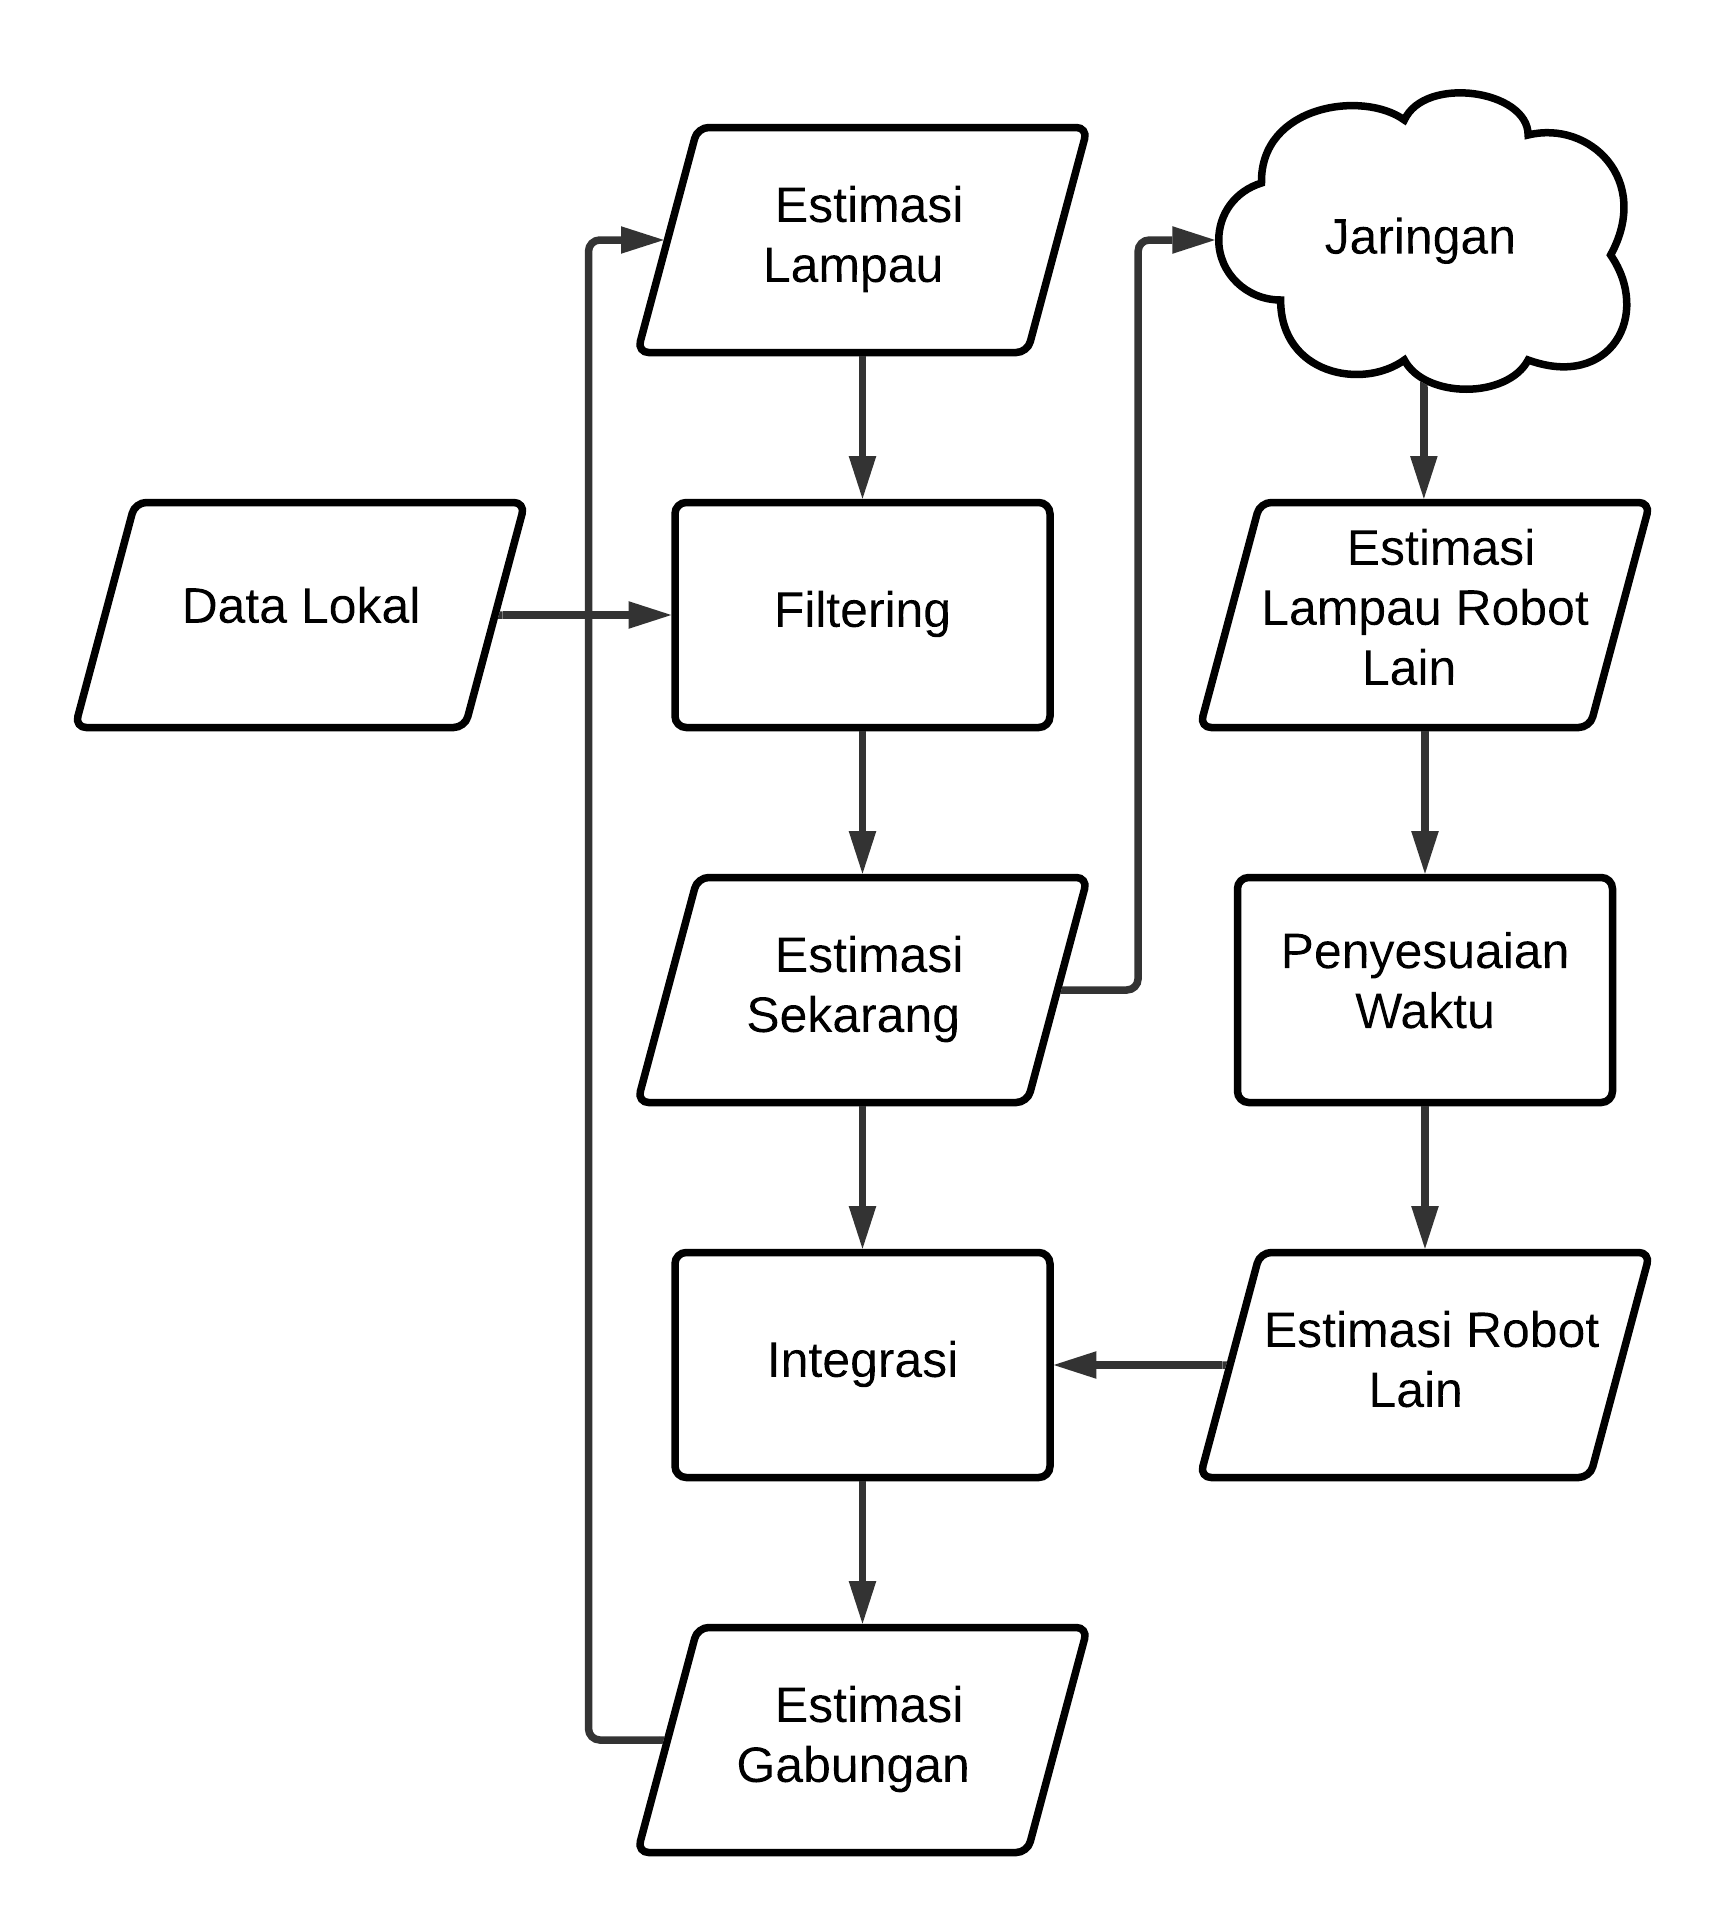
\includegraphics[width=0.8\textwidth]{resources/solution-flowchart.png}
    \caption{Diagram alir hipotesis solusi}
    \label{fig:solution-flowchart}
    \bigskip
\end{figure}

Diagram alir hipotesis solusi digambarkan di \ref{fig:solution-flowchart}. Walaupun terdapat beberapa fungsi \textit{callback} yang dapat berjalan karena \textit{event}nya masing-masing, pemanggilan fungsi \textit{callback} oleh ROS dilakukan secara sinkronis satu-persatu sehingga tidak dibutuhkan pertimbangan mengenai \textit{thread-safety} dan \textit{mutex}. Dengan periode komputasi $30$ ms, \textit{callback} periode komputasi dan \textit{callback} sensor akan dijalankan sekitar $33,3$ kali perdetik dan \textit{callback} data dari teman bergantung pada kondisi jaringan komunikasi akan dijalankan rata-rata maksimal sebanyak $66,6$ kali perdetik, sehingga kinerja algoritma tidak terlalu dituntut dalam segi konstrain waktu komputasi.

\section{Implementasi Algoritma Lokalisasi}

Algoritma estimasi gerakan robot sendiri atau algoritma lokalisasi menggunakan informasi odometri atau perpindahan, orientasi dari kompas, dan persepsi \textit{landmark} untuk mengestimasi dimana dan berapa kecepatan dari robot tersebut sekarang. Selain cara naif yang hanya mengagregasi perpindahan odometri, untuk menggunakan penapis Bayes, model pengukuran dari persepsi \textit{landmark} yang tidak linear terhadap posisi robot sesungguhnya menjadikan penapis Kalman tidak dapat digunakan untuk melakukan lokalisasi ini. Sehingga penapis partikel lebih cocok digunakan untuk menyelesaikan permasalahan ini. Khususnya algoritma \textit{AMCL} yang melakukan \textit{resampling} dianggap sebagai algoritma yang tahan terhadap kemungkinan buruknya pengukuran.

Dalam praktisnya, informasi odometri dapat digunakan baik dalam model transisi maupun model pengukuran dari penapis partikel yang digunakan, sehingga menghasilkan dua variasi dari algoritma lokalisasi yang dapat digunakan, variasi AMCL yang berbasis \textit{pose} atau variasi yang berbasis \textit{pose} dan \textit{twist}.

\subsection{Penapis Partikel Berbasis \textit{Pose}}

Pada variasi pertama, partikel yang digunakan pada penapis partikel lokalisasinya mengandung informasi tentang \textit{pose} sesungguhnya dari robot, sehingga estimasi yang dihasilkan AMCL juga berupa \textit{pose} dari robot. Sedangkan \textit{twist} dari robot diturunkan dengan mengambil perpindahan diantara hasil estimasi sekarang dengan hasil estimasi sebelumnya diturunkan terhadap selisih waktu.

Model transisi dari partikel yang ada menggunakan informasi odometri yang ada, dimana masing-masing partikel digerakan sesuai dengan perpindahan yang disampel di sekitar nilai odometri tersebut.

\begin{algorithm}
    \caption{Model pengukuran \textit{pose}}
    \label{alg:pose-measurement-model}
    \begin{algorithmic}[1]
        \Function{calc\_weight}{pose, compass, landmarks, true\_landmarks}
        \State ln\_vis\_weight = $0$
        \If{size(landmarks) != $0$}
        \State vis\_weight = $0$
        \For{landmark in landmarks}
        \State landmark\_weight = -infinity
        \For{true\_landmark in true\_landmarks}
        \State rel\_landmark = -pose + true\_landmark
        \State weight = exp(compare(landmark, rel\_landmark))
        \State landmark\_weight = max(landmark\_weight, weight)
        \EndFor
        \State vis\_weight += landmark\_weight
        \EndFor
        \State ln\_vis\_weight = log(vis\_weight / size(landmarks))
        \EndIf
        \State ln\_ort\_weight = compare(pose.orientation, compass)
        \State return exp($\alpha \times$ ln\_vis\_weight + $\beta \times$ ln\_ort\_weight)
        \EndFunction
    \end{algorithmic}
\end{algorithm}

Model pengukuran menggunakan informasi \textit{landmark} dimana untuk masing-masing partikel, semua pengukuran \textit{landmark} yang ada dibandingkan dengan semua posisi absolut \textit{landmark} yang sebenarnya untuk diambil peluang terukurnya pengukuran tersebut berdasarkan profil \textit{error} normal independen. Diambil peluang pengukuran terbesar untuk masing-masing pengukuran yang berikutnya dirata-ratakan untuk masing-masing partikel. Selain itu, pengukuran dari kompas berdasarkan distribusi \textit{error} normal dari orientasi sebenarnya juga digunakan. Kedua peluang dari pengukuran \textit{landmark} dan dari pengukuran kompas diintegrasi dengan melakukan perkalian setelah masing-masing peluang dipangkatkan oleh suatu \textit{weight} faktor pengukuran. Fungsi yang digunakan digambarkan pada \ref{alg:pose-measurement-model} dimana fungsi compare menghasilkan logaritma natural dari peluang dilakukannya pengukuran, yang berdasarkan persamaan distribusi normal hanyalah bernilai $-0,5$ dikali jarak kuadrat dibagi dengan variansi.

Hasil prediksi dari suatu iterasi estimasi adalah rata-rata dari partikel yang ada, dimana posisi dirata-ratakan sebagai vektor dan orientasi dirata-ratakan dengan mengambil arah dari rata-rata vektor unit dengan arah orientasi masing-masing partikel. Sedangkan \textit{resampling} dilakukan dengan mengambil \textit{pose} di sekitar rata-rata partikel tersebut ditambah \textit{error} dengan distribusi normal.

\subsection{Penapis Partikel Berbasis \textit{Pose} dan \textit{Twist}}

Pada variasi kedua, partikel yang digunakan mengandung informasi tentang \textit{pose} dan juga \textit{twist} dari robot, sehingga pada variasi ini tidak perlu diturunkan lagi \textit{twist} dari robot secara terpisah karena sudah menjadi bagian dari hasil estimasi penapis.

Pada variasi ini nilai odometri tidak digunakan pada model transisi. Model transisi mengandalkan pada \textit{twist} yang sudah dimiliki masing-masing partikel, dimana \textit{twist} tersebut ditambahkan dengan \textit{error} normal untuk membangkitkan \textit{twist} baru dan \textit{pose} baru dibangkitkan dengan meng\textit{update} \textit{pose} lama menggunakan \textit{twist} yang baru dibangkitkan.

Model pengukuran variasi ini mirip dengan model pada variasi pertama dalam caranya menggunakan pengukuran \textit{landmark} dan kompas. Di variasi ini, odometri juga digunakan pada model pengukuran dengan membandingkannya dengan perpindahan sebenarnya yang dapat didapatkan dari mengintegrasi \textit{twist} partikel dengan selisih waktu.

Rata-rata partikel diambil dengan cara yang sama untuk \textit{pose} dari partikel dan analog untuk mendapatkan rata-rata dari \textit{twist} partikel. \textit{Resampling} juga dilakukan di sekitar \textit{pose} dan \textit{twist} partikel rata-rata dengan penambahan \textit{error}.

\section{Estimasi Gerakan Bola}

Estimasi gerakan bola berdasarkan data persepsi bola yang didapat dari sensor sendiri atau teman lebih leluasa dibandingkan dengan lokalisasi. Hal ini dikarenakan bacaan posisi bola bersifat linear terhadap posisi bola sesungguhnya ditambah suatu \textit{error} seperti yang ada pada asumsi penapis Kalman. Oleh karena itu, walaupun profil \textit{error} sesungguhnya dari bacaan posisi bola tidak \textit{uniform} untuk semua posisi sesungguhnya, dapat dimodelkan \textit{error} normal \textit{uniform} untuk dapat menggunakan penapis Kalman dalam melakukan estimasi gerakan bola. Karena bacaan posisi bola yang dilihat bersifat relatif, maka estimasi gerakan bola mengandalkan estimasi gerakan robot yang melakukan persepsi untuk mengubah bacaan posisi bola yang relatif ke ruang referensi absolut.

\subsection{Estimasi dengan Penapis Kalman}

Penapis Kalman memodelkan distribusi gerakan bola sebagai distribusi normal multivariat dengan vektor rata-rata $\mu$ empat dimensi yang merepresentasikan komponen posisi bola pada sumbu x, kecepatan pada sumbu x, posisi pada sumbu y, dan kecepatan pada sumbu y, juga matriks kovarian $4 \times 4$ dengan urutan komponen yang sama.

Karena informasi bola hanya berupa pengukuran, tidak ada variable transisi yang digunakan dalam estimasi gerakan bola. Sehingga persamaan transisi yang digunakan hanyalah
\begin{align}
    x_t = A_t x_{t-1} + \epsilon_t \,
\end{align}
dimana $A_t$ adalah matriks $4 \times 4$ \textit{update} keadaan dimana posisi baru ditambahkan dengan kecepatan dikalikan selisih waktu, sedangkan $\epsilon_t$ adalah vektor acak \textit{error} empat dimensi. Variansi dari komponen \textit{error} kecepatan adalah konstanta dikali selisih waktu. Karena perubahan posisi adalah perubahan kecepatan dikali selisih waktu, maka didapatkan variansi komponen \textit{error} posisi adalah konstanta dikali selisih waktu pangkat tiga dan kovarian antara komponen \textit{error} posisi dan kecepatan adalah konstanta dikali selisih waktu kuadrat.

Pada persamaan pengukuran $z_t = C_t x_t + \delta_t$, $z_t$ adalah vektor dua dimensi berisi pengukuran posisi absolut bola pada sumbu x dan y. $C_t$ adalah matriks pengukuran berdimensi $2 \times 4$ yang bernilai $1$ di komponen posisi yang terkait dan $0$ di sisanya. Walaupun distribusi \textit{error} pengukuran bola tergantung dari posisi robot yang melihat dan jarak bola dengan robot, karena dibutuhkan suatu vektor acak $\delta_t$ yang sama atau \textit{uniform} untuk semua posisi, maka digeneralisasi $\delta_t$ sebagai vektor dua dimensi dengan matriks kovariansi $Q_t$ merupakan matriks identitas dikali suatu konstanta.

\subsection{Estimasi dengan Penapis Partikel}

Estimasi gerakan bola dengan penapis partikel mirip dengan algoritma lokalisasi variansi dua, dimana sampel berisi posisi dan kecepatan dari bola dan tidak ada kalkulasi terpisah untuk menentukan kecepatan dari bola. Tidak ada variabel transisi yang dapat digunakan, jadi model transisi hanyalah membangkitkan kecepatan baru di sekitar kecepatan partikel dan meng\textit{update} posisi berdasarkan kecepatan baru dan selisih waktu seperti pada lokalisasi variansi dua.

Model pengukuran menggunakan persamaan yang sama dengan pengukuran menggunakan \textit{landmark}, dimana posisi robot yang melakukan persepsi mengandalkan hasil lokalisasi untuk menghasilkan posisi relatif bola referensi untuk dibandingkan dengan posisi relatif bola yang dilihat.

\section{Integrasi Data Bola Terlambat}

Cara integrasi data bola dari teman yang paling dasar adalah dengan mengintegrasinya ke dalam penapis bola yang digunakan, sama seperti dengan pemrosesan data sensor, apabila dilihat bahwa \textit{timestamp} dari data tersebut lebih baru daripada data terakhir yang sudah diproses. Kekurangan dari metode ini adalah apabila robot sendiri dan satu atau lebih teman melihat bola pada saat yang sama, informasi yang didapat dari teman tersebut tidak akan pernah digunakan karena data sensor dari robot sendiri hampir pasti sampai lebih cepat dibandingkan dengan data dari teman yang ditambahkan dengan latensi komunikasi. Salah satu cara untuk menangani hal ini adalah dengan menggunakan modifikasi penapis untuk \textit{out of order measurement} atau (\textit{OOSM}).

\subsection{Estimasi dengan OOSM-PF}

Karena tidak ada konstrain waktu ataupun memori yang signifikan, penanganan data terlambat dapat dilakukan menggunakan penyimpanan dan penyisipan data pengukuran. Pada penapis partikel OOSM-PF, untuk batas jumlah yang telah ditentukan sebelumnya, beberapa data pengukuran dan \textit{state} estimasi yang terakhir disimpan secara terurut berdasarkan \textit{timestamp} datanya. Sistem penyimpanan dapat menggunakan tipe data seperti \textit{map} terurut yang menyimpan datanya secara terurut berdasarkan \textit{key}nya yang diimplementasi di atas tipe data seperti \textit{red-black tree}. Dalam kasus penapis partikel, \textit{state} yang dimaksud adalah kumpulan partikel dalam penapis dan nilai dari $w_fast$ dan $w_slow$.

Apabila ditemui data terlambat yang lebih lama dari data terlama yang disimpan, maka data tersebut dibuang dan dikembalikan hasil estimasi terakhir. Apabila data tersebut lebih baru, cari data paling baru yang disimpan yang lebih lama dari data terlambat tersebut. Lalu simpan data terlambat tersebut dengan menghitung \textit{state}nya menggunakan algoritma penapis partikel biasa menggunakan \textit{state} sebelumnya dari data paling baru tersebut. \textit{Update} juga semua \textit{state} dari data yang disimpan yang ada setelah data yang baru dimasukan, dan buang data terlama yang disimpan apabila sudah melebihi jumlah maksimal data yang disimpan.

Kompleksitas waktu dan ruang dari algoritma ini berkembang secara linear terhadap batas jumlah data yang disimpan. Akan tetapi karena data yang sudah melewati beberapa periode komputasi semakin lama tidak relevan, maka batas jumlah ini tidak perlu diatur dengan besar.

\subsection{Estimasi OOSM-PF dengan Data Bola Opsional}

Karena kegagalan persepsi bola oleh robot juga sebenarnya memberikan informasi mengenai posisi bola dimana kegagalan posisi bola yang sebenarnya kemungkinan berada di luar radius penglihatan robot, maka dapat dibuat variasi dari penapis partikel bola yang dapat menerima data bola secara opsional. Pemanggilan penapis partikel tanpa adanya informasi bola yang menandakan bahwa kemungkinan bola berada di luar radius penglihatan mengakibatkan algoritma model pengukuran meninggikan \textit{weight} partikel yang berada di luar radius penglihatan dan mengurangi \textit{weight} partikel yang berada di dalam radius penglihatan.

Algoritma ini hanya mungkin berfungsi dengan baik menggunakan modifikasi data \textit{OOSM}. Ini disebabkan karena jika digunakan cara integrasi dasar yang hanya mempertimbangkan \textit{timestamp}, maka robot hanya akan mempertimbangkan data dari sensor sendiri saja walaupun bola tidak terlihat, karena informasi dari teman yang hampir pasti terlambat walaupun mungkin teman tersebut melihat posisi bola sehingga informasinya lebih berguna dibandingkan informasi robot sendiri yang tidak melihat bola.

\subsection{Estimasi dengan OOSM-KF}

OOSM-KF adalah algoritma seperti OOSM-PF akan tetapi menggunakan algoritma penapis Kalman sebagai dasarnya. Perbedaan dari algoritma ini adalah \textit{state} yang disimpan hanyalah berupa representasi distribusi normal multivariat berupa vektor rata-rata dan matriks kovariansi, sehingga kompleksitas waktu dan ruangnya setaraf lebih efisien dibandingkan OOSM-PF.

\subsection{Estimasi OOSM-KF dengan Data Bola Kombinasi}

Salah satu cara konvensional untuk menggabungkan data posisi bola dari banyak robot adalah dengan merata-ratakan data tersebut. Variansi OOSM-KF dengan data bola kombinasi adalah variansi OOSM-KF bola dimana apabila diterima dua atau lebih data dengan \textit{timestamp} yang sama dari beberapa robot, maka data tersebut tidak akan diproses satu-persatu, melainkan dengan dirata-ratakan dan diproses dengan sekaligus. Variansi ini menggunakan penapis Kalman karena rata-rata posisi absolut bola yang digunakan dengan kemungkinan bola dilihat lebih dari satu robot, sehingga penapis partikel yang membutuhkan satu robot yang melihat bola untuk menentukan profil \textit{error} dari bacaan tidak dapat digunakan.

\section{Koreksi Gerakan Robot Teman dengan Persepsi \textit{Vision}}

Walaupun hasil persepsi robot teman dari suatu robot memiliki \textit{error} yang cukup tinggi jika dibandingkan dengan hasil lokalisasi oleh teman tersebut menggunakan odometri, kompas, dan beberapa persepsi \textit{landmark}, hasil persepsi tersebut lebih tersedia karena bersumber dari sensor sendiri jika dibandingkan dengan hasil lokalisasi teman yang harus melalui latensi jaringan, terutama apabila kondisi jaringan yang sedang buruk. Oleh karena itu, persepsi robot teman menjadi informasi yang berguna karena dapat digunakan untuk mengoreksi estimasi robot sendiri mengenai gerakan robot teman.

Karena informasi hasil lokalisasi teman tersebut tetap lebih berharga dibandingkan persepsi melalui \textit{vision}, digunakan OOSM-PF untuk mencampurkan data dari teman yang terlambat dengan persepsi \textit{vision} yang selalu ada. Algoritma penapis partikel yang digunakan menyediakan dua jenis antarmuka fungsi estimasi, yaitu fungsi yang menerima data dari teman berupa \textit{pose} dan \textit{twist} secara absolut dan fungsi yang menerima data dari sensor berupa posisi relatif teman tersebut. Walaupun model transisinya sama, model pengukuran dari data teman membandingkan jarak nilai \textit{pose} dan \textit{twist} estimasi dan partikel, sedangkan model pengukuran dari data sensor sama seperti penapis partikel bola yang membandingkan posisi relatif robot teman referensi dengan yang dilihat.

Sensor \textit{vision} yang tidak dapat membedakan teman yang mana yang sedang dilihat mengakibatkan kebutuhan suatu algoritma yang dapat menentukan siapa robot teman yang dilihat berdasarkan posisinya. Dibuat matriks \textit{cost} yang menyimpan \textit{cost} dalam mencocokan suatu persepsi teman dengan identitas robot teman tersebut. \textit{Cost} berupa jarak kuadrat dari posisi absolut persepsi robot teman tersebut dengan estimasi posisi sesungguhnya suatu identitas robot teman berdasarkan estimasi yang sudah disesuaikan waktunya. Dari sini, masalah penyeleksian identitas teman dapat diselesaikan dengan algoritma seperti \textit{Hungarian algorithm}, tetapi untuk kasus kemungkinan robot teman yang sedikit, dapat langsung di\textit{brute-force} untuk menentukan penyeleksian dengan jumlah \textit{cost} minimum.

\chapter{EKSPERIMEN DAN ANALISIS}

Bab ini menjelaskan mengenai implementasi dan prosedur pengujian algoritma estimasi, perbandingan hasil dari pengujian, dan analisis dari hasil tersebut.

\section{Skenario Pengujian}

Tujuan dari pengujian adalah untuk membandingkan kinerja dari algoritma estimasi yang dipilih dan mendapatkan algoritma estimasi yang paling baik dalam menyelesaikan masalah estimasi gerakan robot tim dan bola dalam kondisi latensi komunikasi.

Pengujian algoritma estimasi dilakukan di lingkungan simulasi yang dibangun pada \textit{framework} ROS yang dibahas di bab sebelumnya. \textit{Node-node} yang berfungsi untuk menjalankan simulasi dan estimasi yaitu \textit{node} simulasi \textit{world state}, simulasi sensor, \textit{world model}, dan simulasi komunikasi ditulis dalam bahasa C++17 yang di\textit{compile} menggunakan gcc dengan optimasi -O3, sedangkan \textit{node} aggregator dan evaluator yang bertugas untuk mengagregasi dan mengambil statistik dari data, beserta melakukan visualisasi ditulis dalam bahasa Python 3 menggunakan \textit{library} matplotlib. Beberapa \textit{node} tambahan juga digunakan seperti \textit{node} \textit{timer} untuk menyelesaikan simulasi setelah waktu tertentu, dan \textit{node} untuk menyimpan konfigurasi dan merekam eksekusi simulasi agar simulasi dapat ditampilkan ulang.

Berikut adalah spesifikasi \textit{hardware} yang digunakan dalam pengujian di lingkungan simulasi:
\begin{enumerate}
    \item OS Ubuntu 20.04.3 LTS
    \item CPU Intel(R) Core(TM) i7-9750H CPU @ 2.60GHz (12 CPUs)
    \item RAM 16 GB
\end{enumerate}

Pengujian dilakukan dengan mengambil statistik metrik \textit{error} berupa jarak dari estimasi masing-masing robot dibandingkan dengan \textit{world state} yang sesungguhnya. Masing-masing jenis \textit{world model} dijalankan sebanyak lima kali tiga menit waktu berjalannya program, sehingga didapatkan sekitar $5 \times 3 \times 60 \times 1000 : 30 = 30000$ banyak nilai per statistik yang akan dianalisis menggunakan ringkasan lima angkanya dan statistik lain seperti rata-rata.

Skenario pengujian dapat dijalankan dalam tiga jenis kondisi jaringan, yaitu:
\begin{enumerate}
    \item Kondisi baik dengan $80\%$ keadaan jaringan baik
    \item Kondisi sedang dengan $50\%$ keadaan jaringan baik
    \item Kondisi buruk dengan $20\%$ keadaan jaringan baik
\end{enumerate}

Untuk perbandingan kinerja algoritma, diiterasi beberapa jenis \textit{node} \textit{world model} dengan variasi algoritma estimasi yang berbeda-beda dengan iterasi sebelumnya:
\begin{enumerate}
    \item \textit{world model} O dimana lokalisasi dan estimasi dilakukan dengan naif
    \item \textit{world model} P yang melakukan lokalisasi dengan penapis partikel \textit{pose} dan estimasi bola menggunakan penapis Kalman
    \item \textit{world model} Q yang melakukan lokalisasi dengan penapis partikel \textit{pose} dan \textit{twist}
    \item \textit{world model} R yang mengestimasi bola menggunakan penapis partikel
    \item \textit{world model} RB yang tidak melakukan penyesuaian waktu saat mengirimkan hasil estimasi
    \item \textit{world model} S yang mengestimasi bola dengan OOSM-PF
    \item \textit{world model} SB yang mengestimasi bola dengan OOSM-PF dengan data opsional
    \item \textit{world model} SC yang mengestimasi bola dengan OOSM-KF
    \item \textit{world model} SD yang mengestimasi bola dengan OOSM-KF dengan data kombinasi
    \item \textit{world model} T yang mengoreksi lokasi teman menggunakan data \textit{vision}
\end{enumerate}

\section{Pengujian dan Analisis Algoritma Estimasi Dasar}

\subsection{Perbandingan Algoritma tanpa Penapis dan dengan Penapis}

\textit{World model} O yang melakukan lokalisasi dengan naif dengan mengakumulasi nilai odometri tanpa koreksi \textit{vision} dan menggunakan data persepsi bola dengan mentah dibuat sebagai pembanding paling dasar dengan algoritma dengan penapis sederhana.

\textit{World model} P menggunakan penapis partikel berbasis \textit{pose} untuk lokalisasinya dan penapis Kalman untuk mengestimasi posisi bola. Data dari teman digunakan secara mentah dan data bola dimasukan ke dalam penapis apabila \textit{timestamp}nya lebih baru. Dilakukan penyesuaian waktu dari \textit{timestamp} data ke waktu saat ini saat hasil estimasi objek dikirimkan.

\begin{figure}[p]
    \centering
    \medskip
    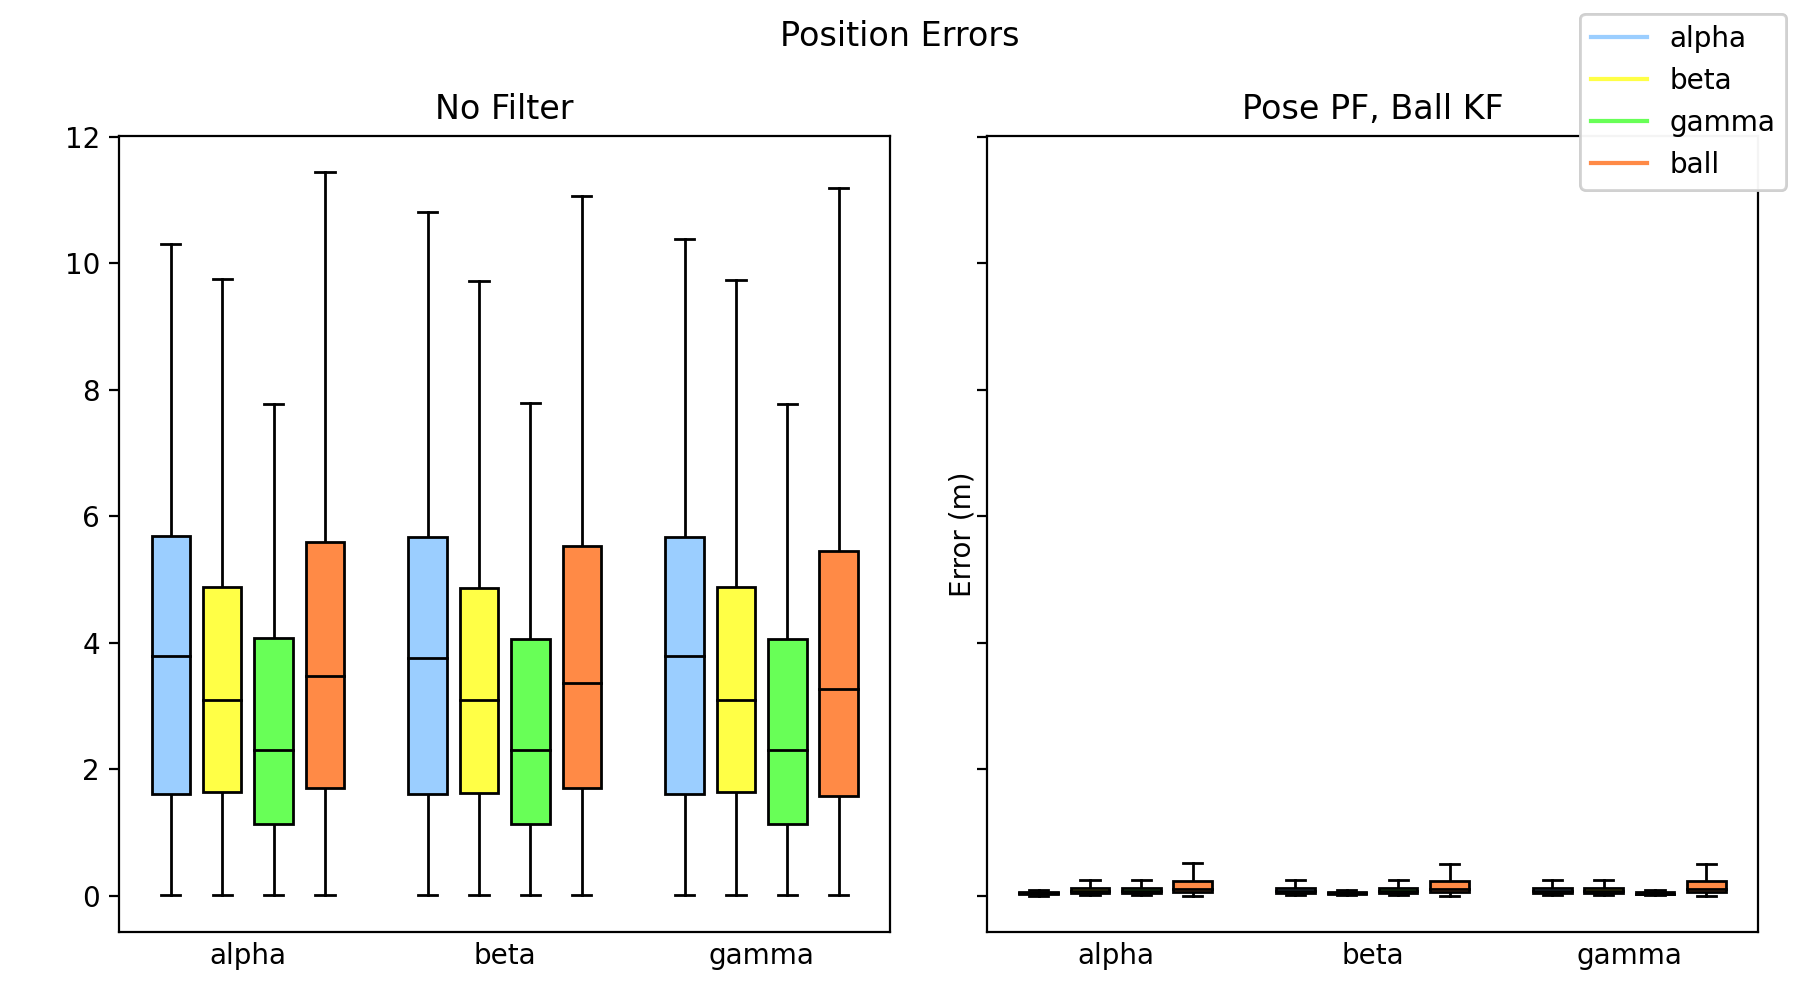
\includegraphics[width=0.9\textwidth]{resources/cfg1_AO_AP_error_pos.png}
    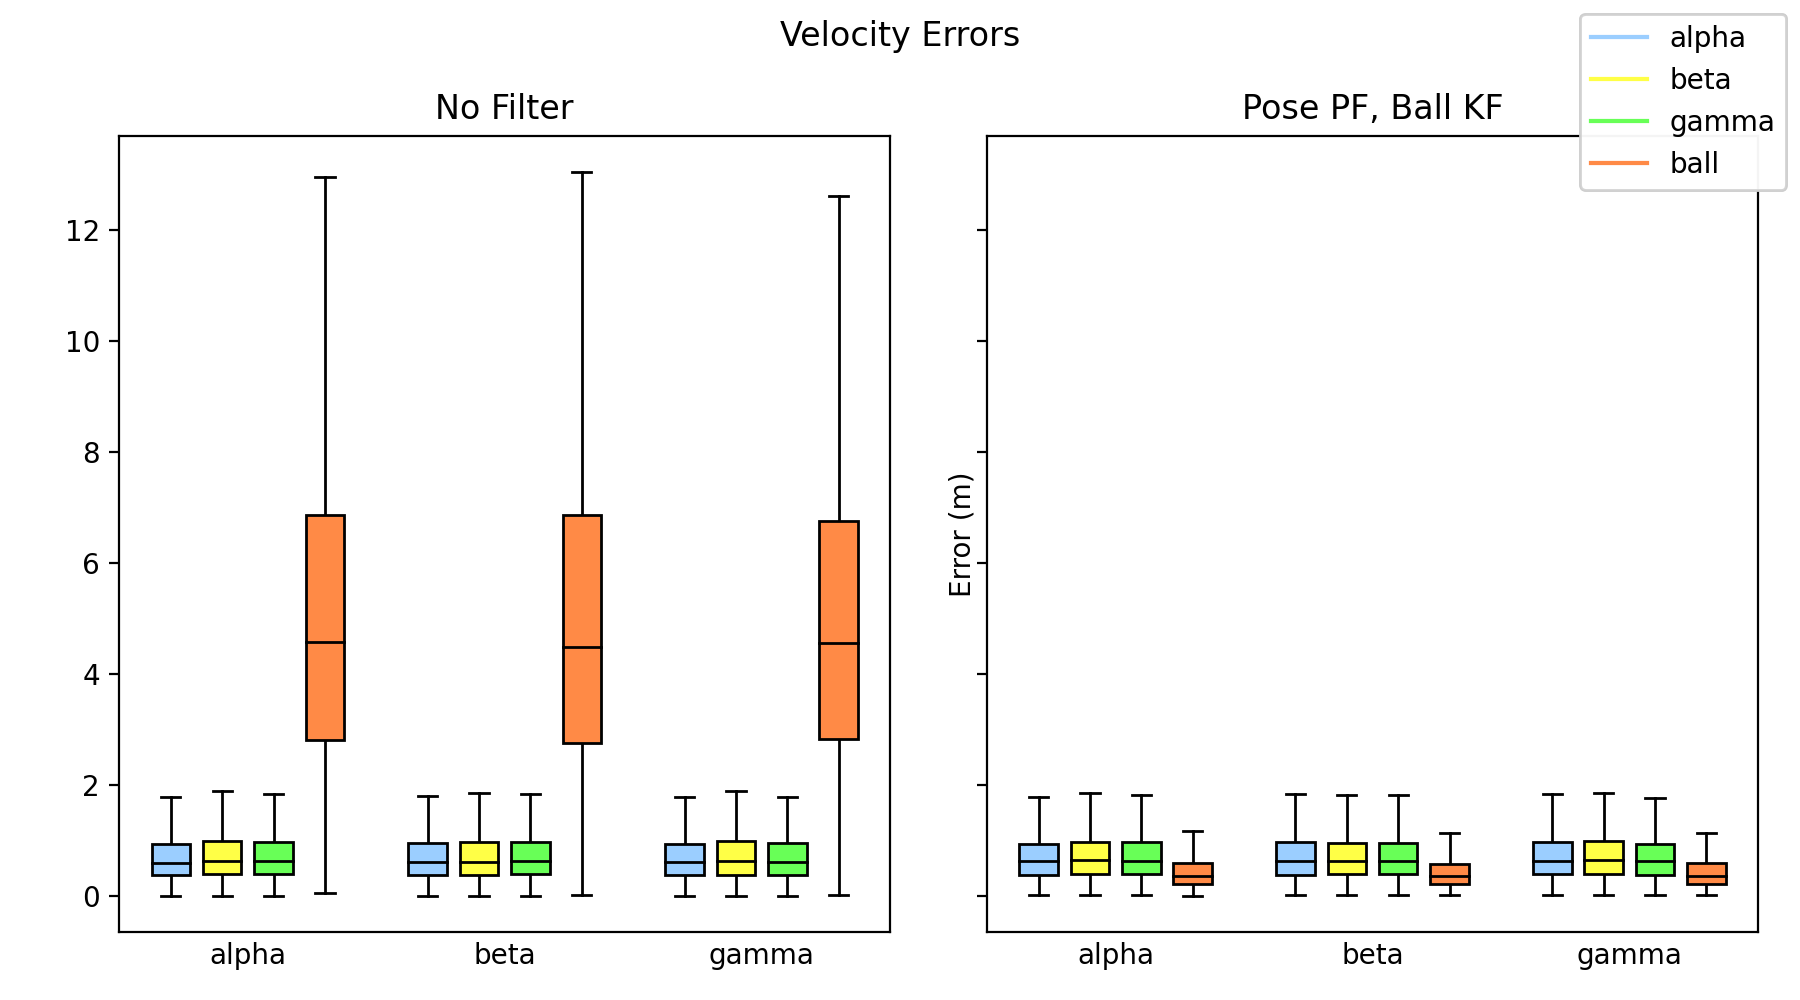
\includegraphics[width=0.9\textwidth]{resources/cfg1_AO_AP_error_vel.png}
    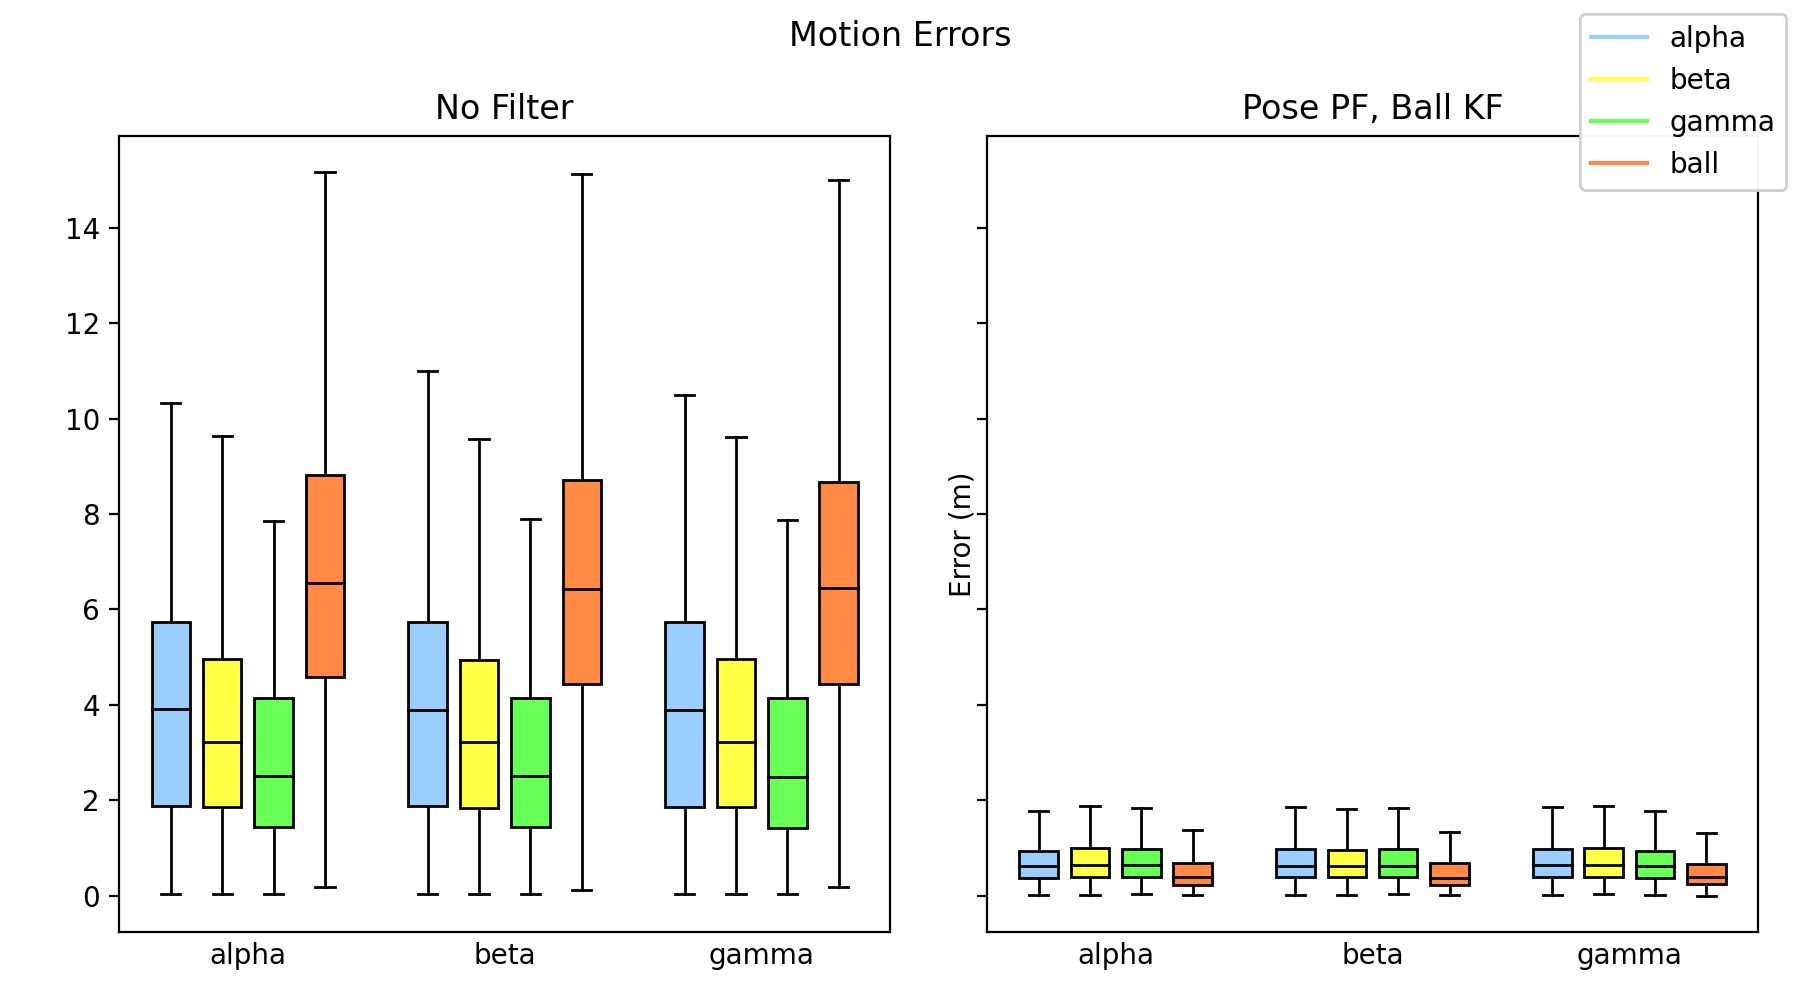
\includegraphics[width=0.9\textwidth]{resources/cfg1_AO_AP_error_motion.png}
    \caption{\textit{Error} \textit{world model} O dan P jaringan baik}
    \label{fig:1-o-p-error}
    \bigskip
\end{figure}

Dari grafik \ref{fig:1-o-p-error} dapat dilihat bahwa ada peningkatan yang sangat signifikan dalam akurasi lokalisasi robot. Dari diagonal lapangan yang sepanjang $10,82$ meter, \textit{world model} O mendapat \textit{error} yang tersebar dalam rentang sebesar itu. Sehingga perbandingan ini menggambarkan seberapa berisiknya \textit{error} sensor yang terakumulasi dalam bacaan odometri seperti sensor lainnya, sedangkan didapatkan bahwa tidak ada perbedaan yang signifikan dari estimasi kecepatan pada penapis partikel berbasis \textit{pose} dan \textit{noise} dari \textit{error} mentah bacaan odometri. Untuk kecepatan bola, karena kecepatan diturunkan dari selisih posisi, masuk akal bahwa estimasi posisi yang lebih baik akan menghasilkan estimasi kecepatan yang lebih baik juga.

\subsection{Perbandingan Algoritma Lokalisasi Penapis Partikel Berbasis \textit{Pose} dan Penapis Partikel Berbasis \textit{Twist}}

Dibandingkan dengan \textit{world model} P, \textit{world model} Q menggunakan penapis partikel berbasis \textit{pose} dan \textit{twist} untuk melakukan lokalisasi, dibanding \textit{pose} saja.

\begin{figure}[p]
    \centering
    \medskip
    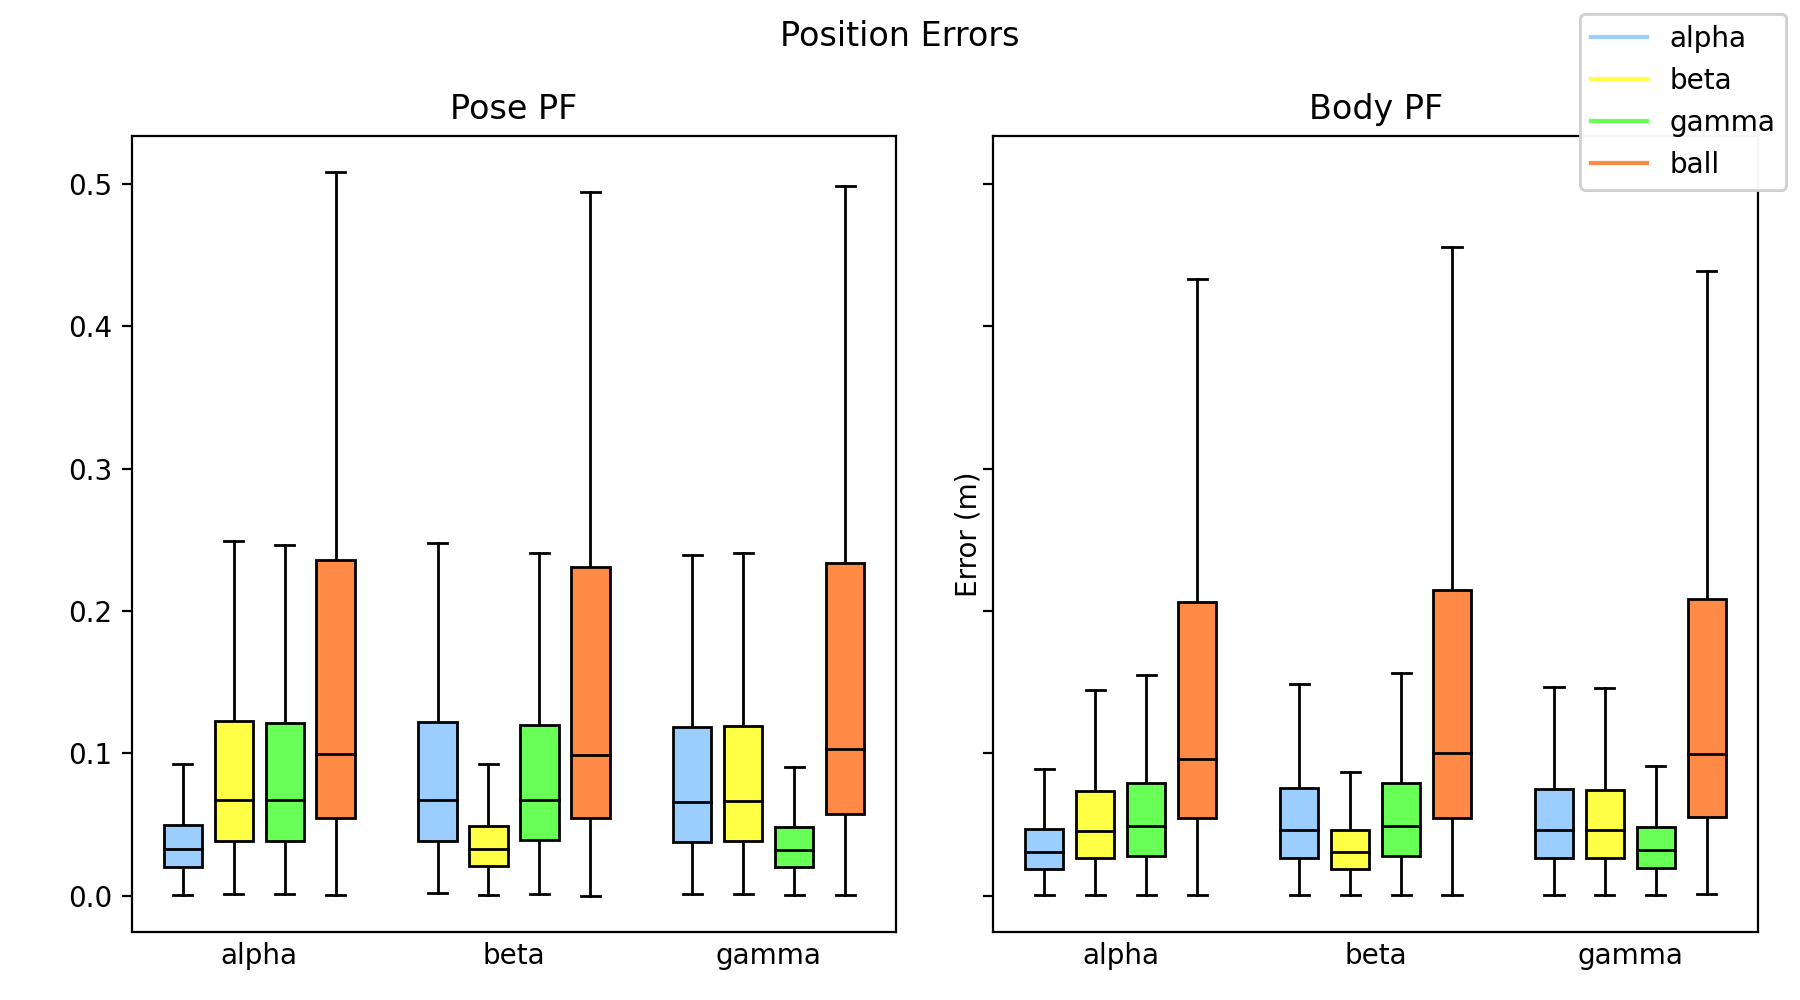
\includegraphics[width=0.9\textwidth]{resources/cfg1_AP_AQ_error_pos.png}
    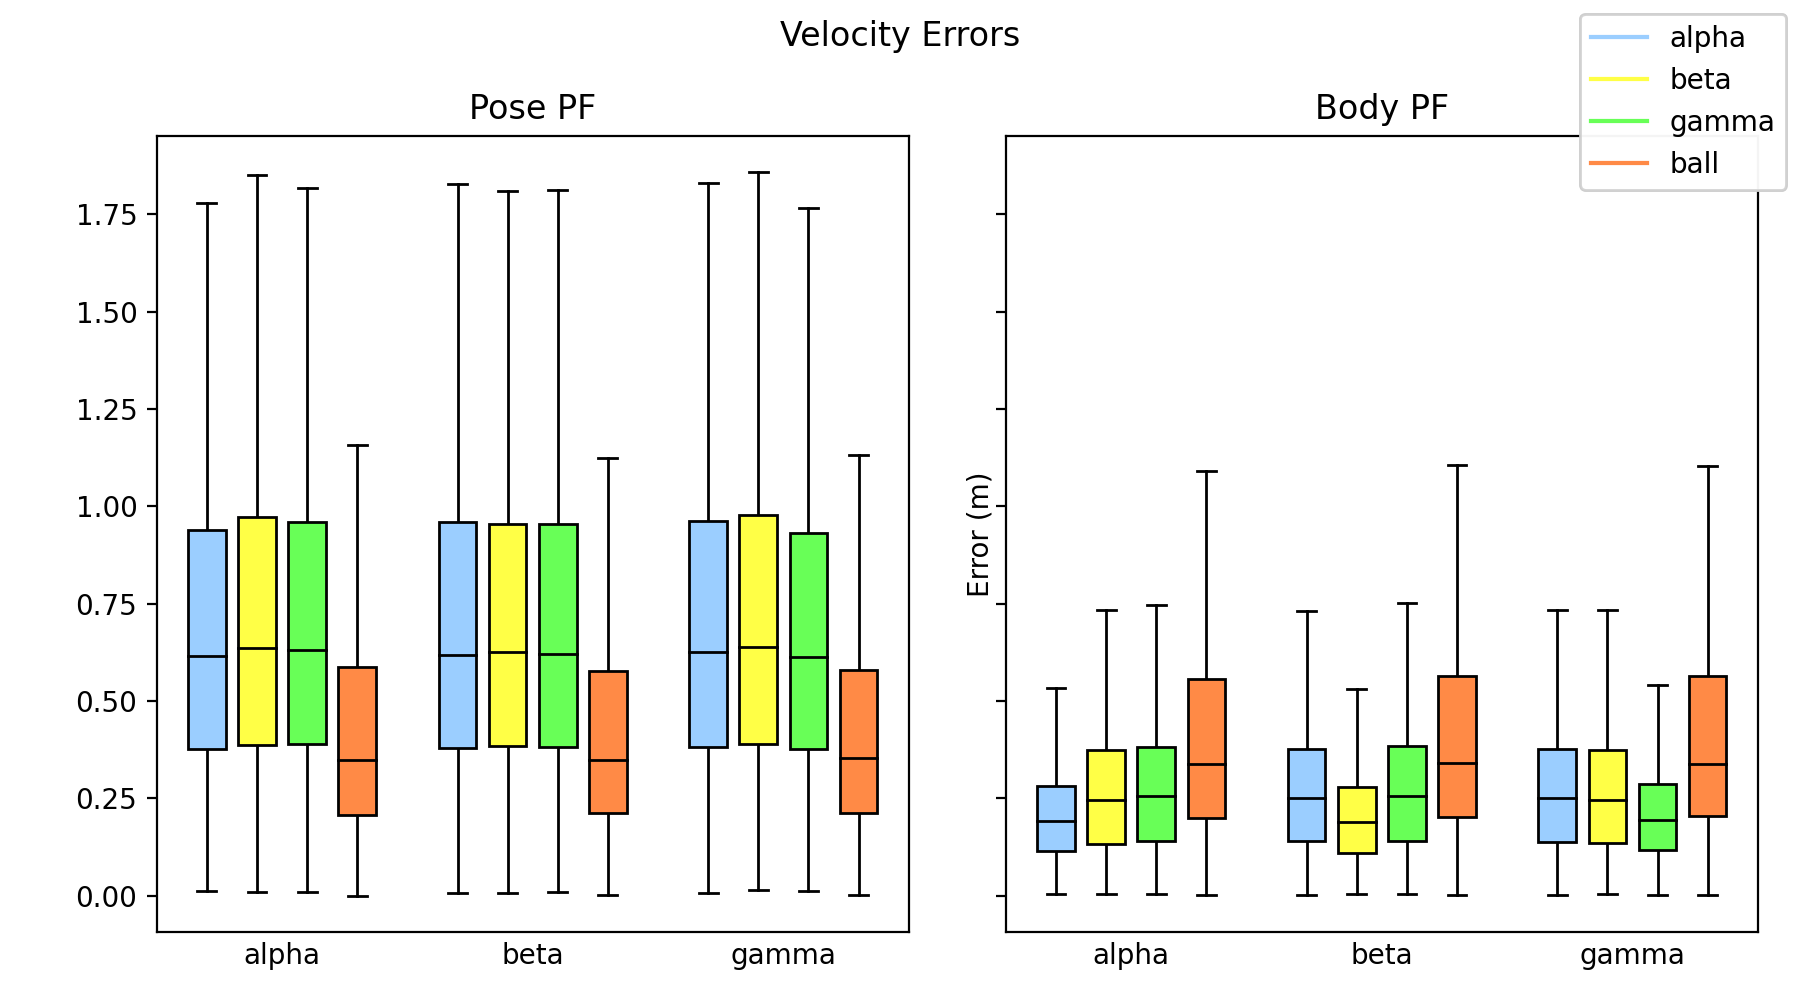
\includegraphics[width=0.9\textwidth]{resources/cfg1_AP_AQ_error_vel.png}
    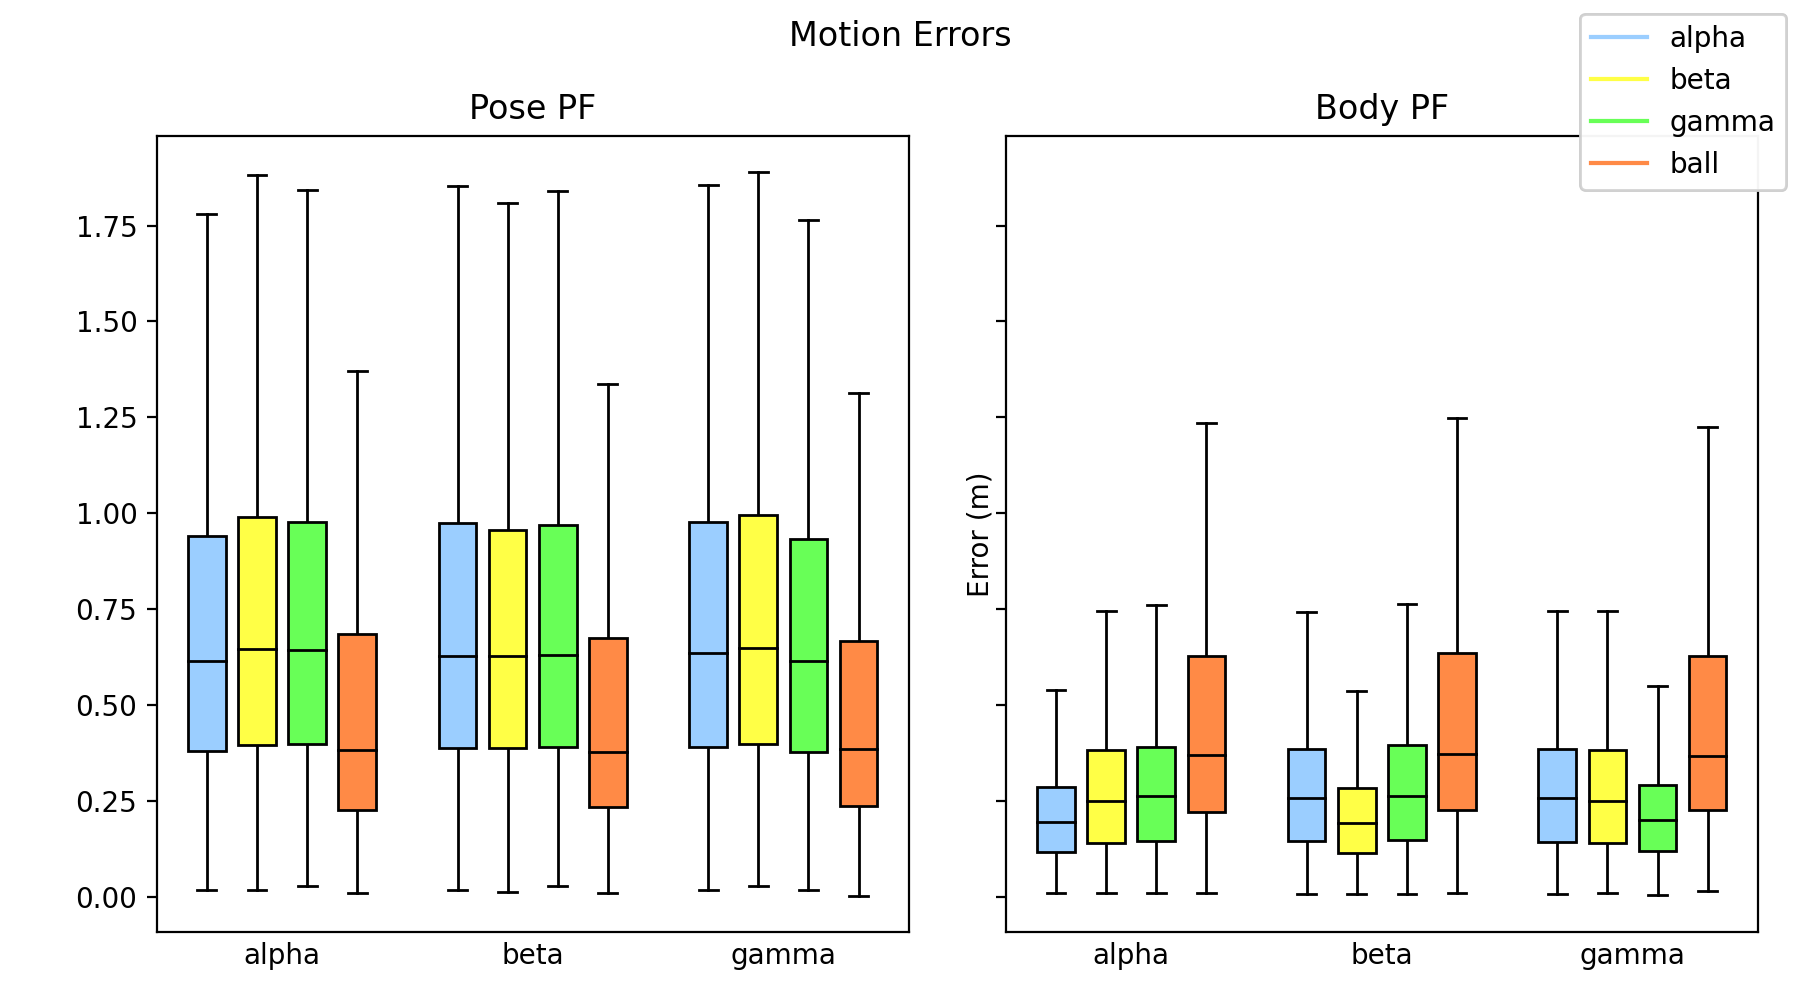
\includegraphics[width=0.9\textwidth]{resources/cfg1_AP_AQ_error_motion.png}
    \caption{\textit{Error} \textit{world model} P dan Q jaringan baik}
    \label{fig:1-p-q-error}
    \bigskip
\end{figure}

Pada grafik \ref{fig:1-p-q-error}, didapatkan bahwa penapis partikel berbasis \textit{pose} dan \textit{twist} dapat memiliki performa yang lebih baik, terutama dalam mengestimasi \textit{twist} dimana median \textit{error} yang didapat sekitar tiga kali lipat lebih baik. Karena penapis partikel berbasis \textit{pose} tidak melacak \textit{twist} dalam partikelnya mengakibatkan penapis tidak mengetahui pergerakan jangka panjang dari robot dan hanya memaksimalkan informasi persepsi \textit{landmark} dan kompasnya saja, sehingga tidak dapat seakurat penapis berbasis \textit{pose} dan \textit{twist}. Perhatikan juga dari grafik posisi bahwa peningkatan akurasi dari lokalisasi dapat meningkatkan akurasi dari estimasi gerakan bola, walaupun sedikit, karena estimasi bola bergantung pada hasil lokalisasi.

\subsection{Perbandingan Algoritma Estimasi Bola Menggunakan Penapis Kalman dan Penapis Partikel}

Dibandingkan dengan \textit{world model} Q, \textit{world model} R menggunakan penapis partikel untuk mengestimasi gerakan dari bola, daripada menggunakan penapis Kalman.

\begin{figure}[p]
    \centering
    \medskip
    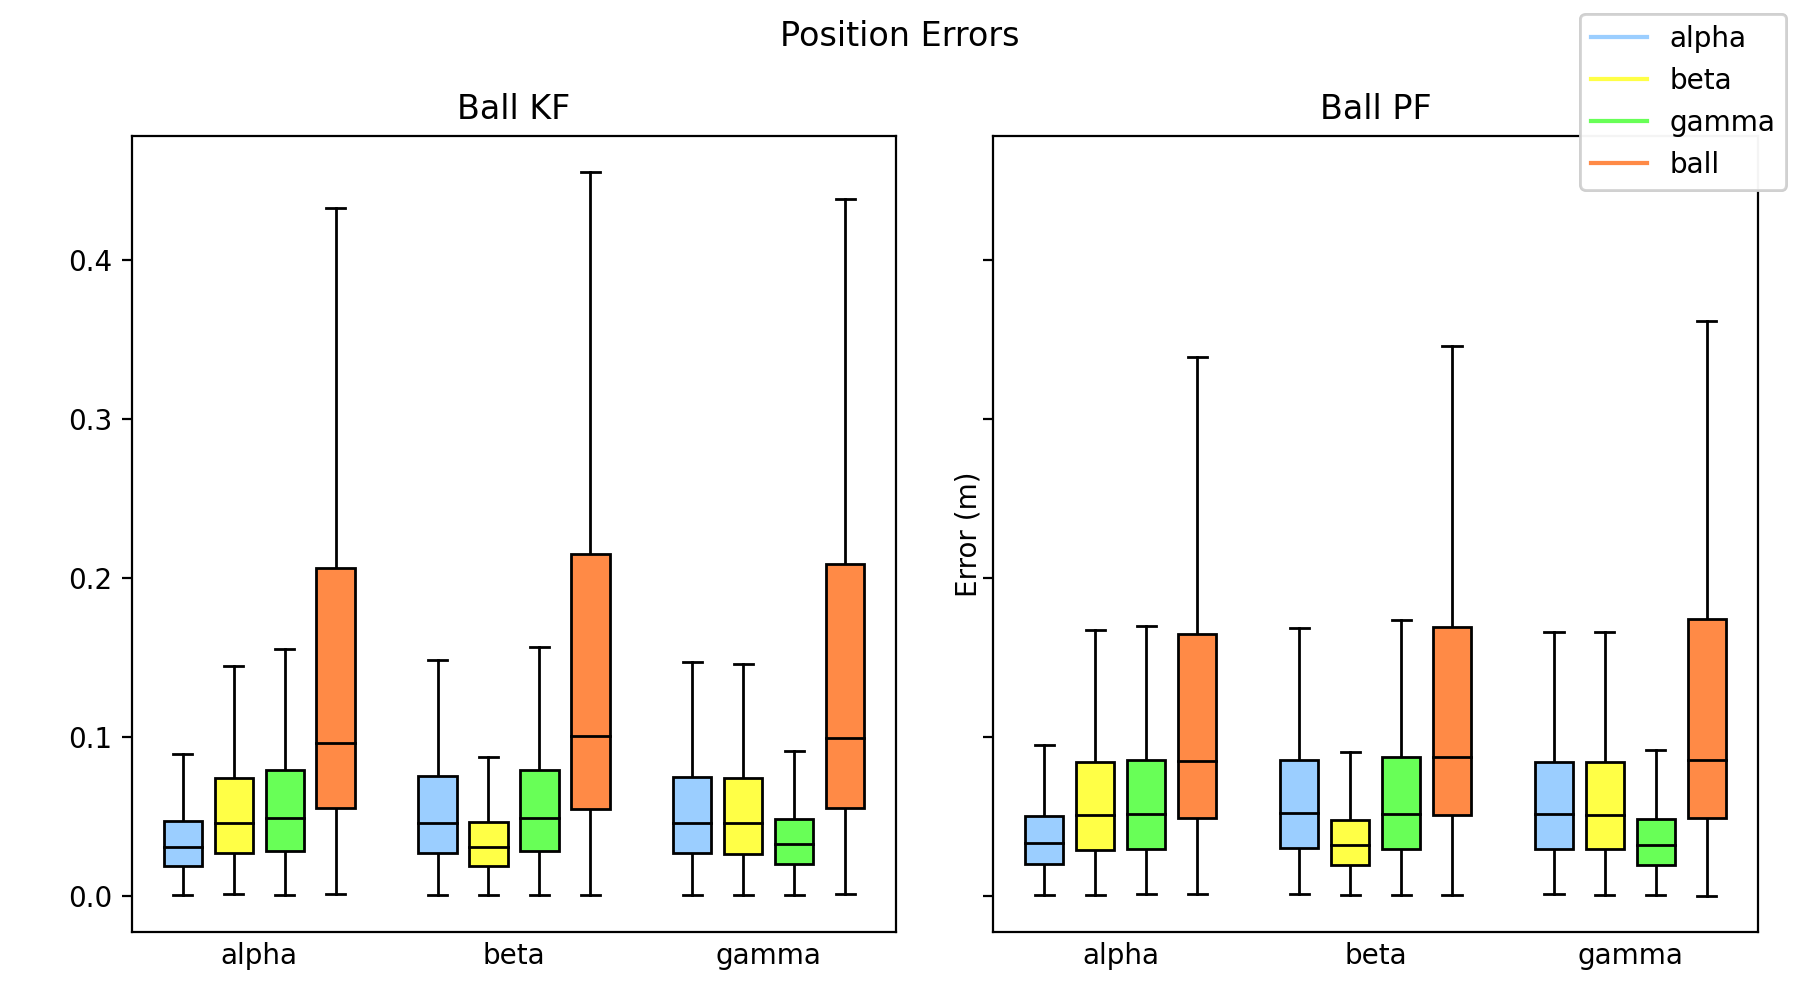
\includegraphics[width=0.9\textwidth]{resources/cfg1_AQ_AR_error_pos.png}
    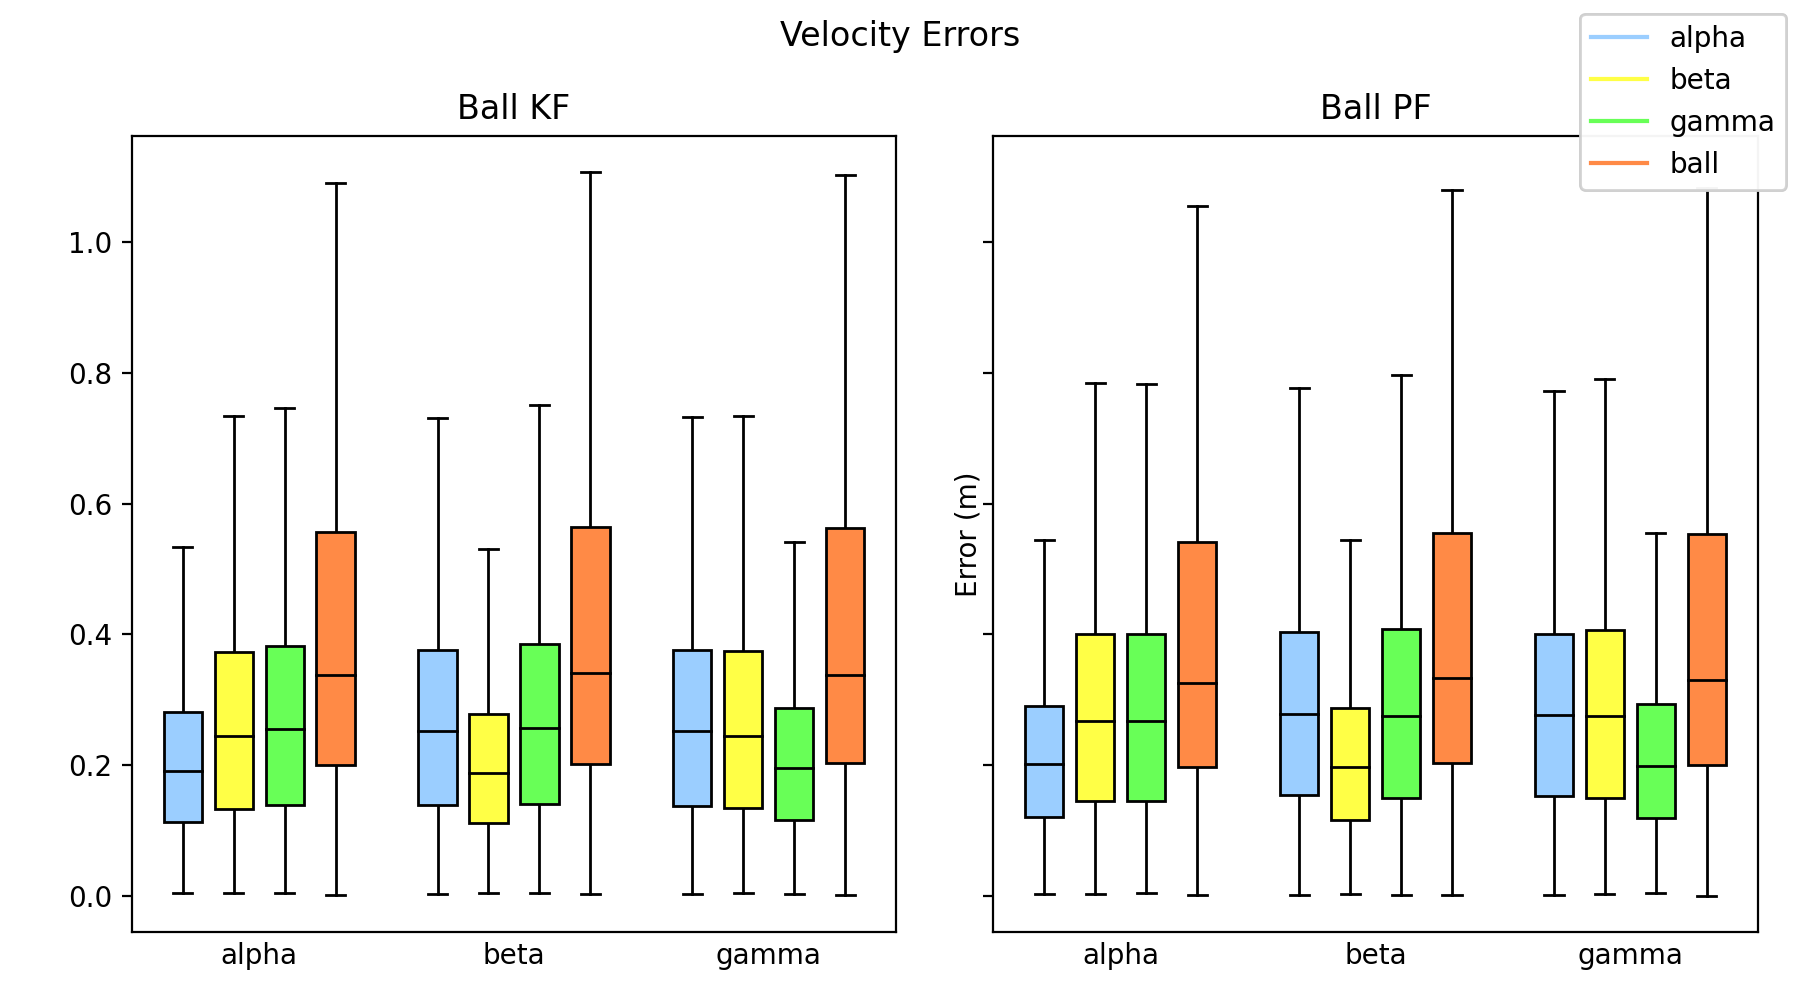
\includegraphics[width=0.9\textwidth]{resources/cfg1_AQ_AR_error_vel.png}
    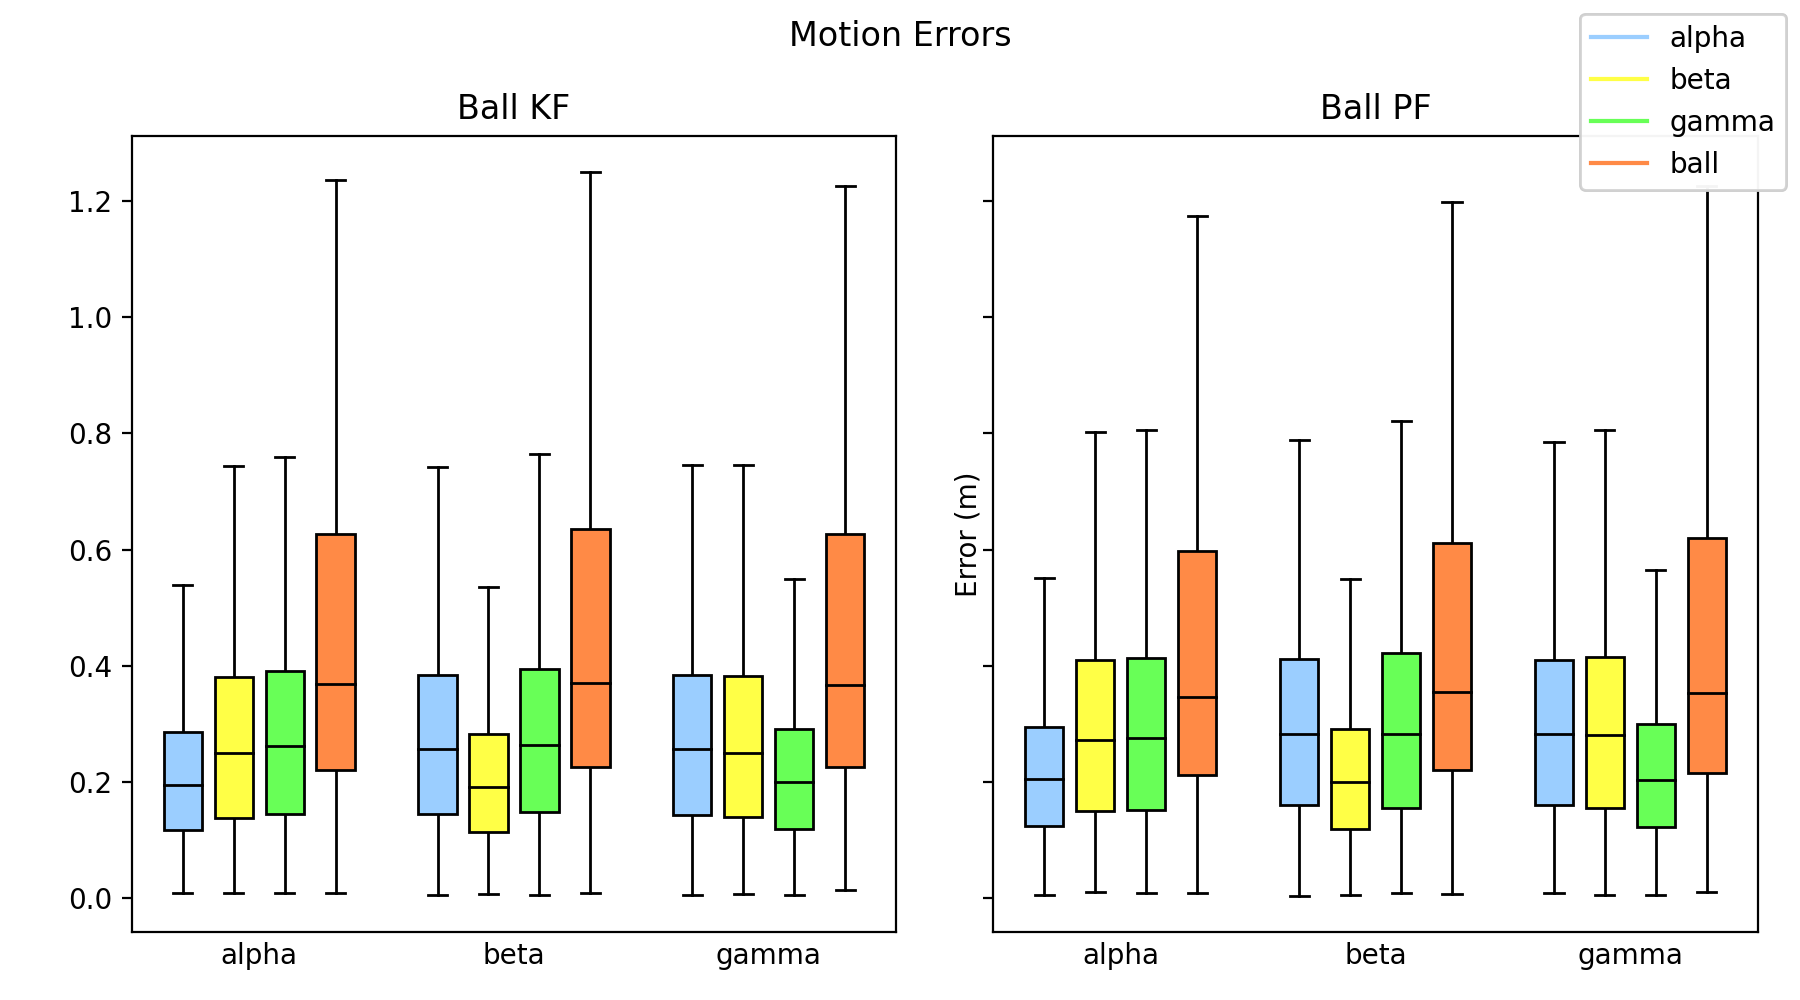
\includegraphics[width=0.9\textwidth]{resources/cfg1_AQ_AR_error_motion.png}
    \caption{\textit{Error} \textit{world model} Q dan R jaringan baik}
    \label{fig:1-q-r-error}
    \bigskip
\end{figure}

Pada grafik \ref{fig:1-q-r-error}, terdapat peningkatan kecil dalam penggunaan penapis partikel dibanding dengan menggunakan penapis Kalman. Hal ini tampaknya disebabkan karena pemodelan pengukuran pada penapis Kalman yang tidak eksak sama dengan profil \textit{error} dari \textit{vision} yang membedakan \textit{error} sejajar dan tegak lurus dengan besar tergantung dari jarak objek, jika dibandingkan dengan penapis partikel yang dapat dengan eksak memodelkan profil \textit{error} tersebut.

\subsection{Perbandingan Algoritma dengan Penyesuaian Waktu dan tanpa Penyesuaian Waktu}

Dibandingkan dengan \textit{world model} R, \textit{world model} RB dibuat tanpa melakukan penyesuaian waktu antara \textit{timestamp} data estimasi dan waktu sekarang saat mengirimkan hasil estimasi ke evaluator.

\begin{figure}[p]
    \centering
    \medskip
    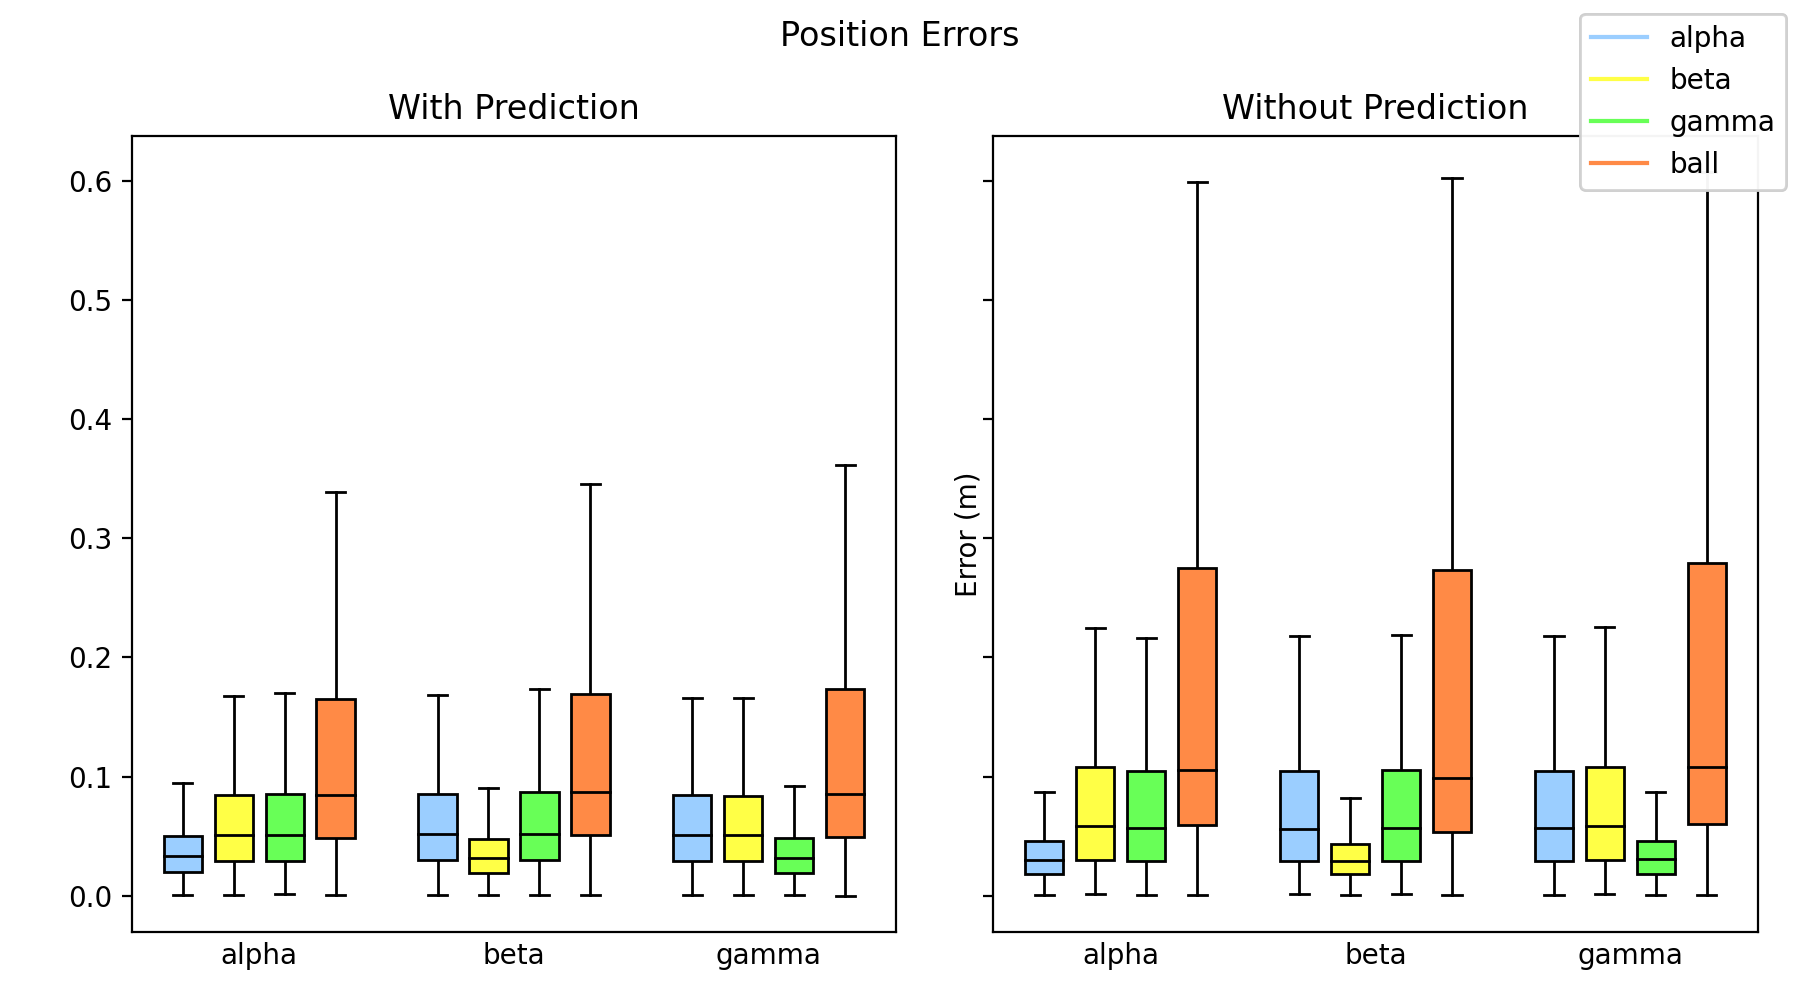
\includegraphics[width=0.9\textwidth]{resources/cfg1_AR_ARB_error_pos.png}
    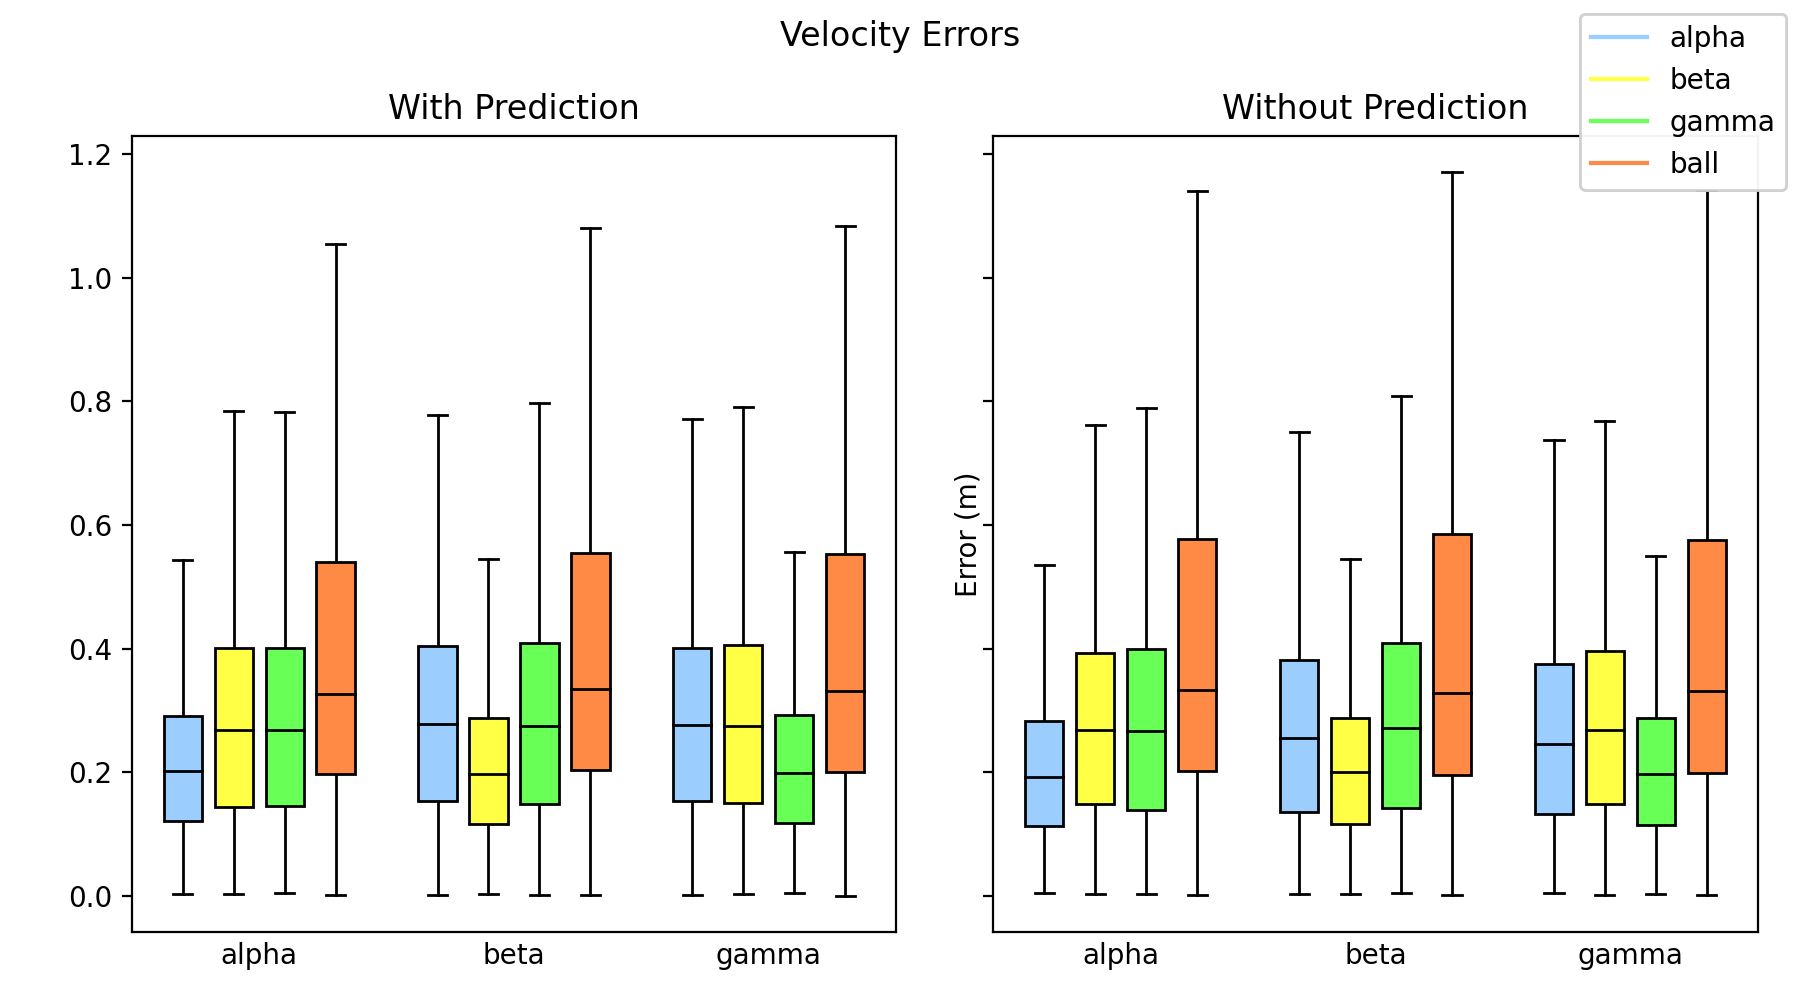
\includegraphics[width=0.9\textwidth]{resources/cfg1_AR_ARB_error_vel.png}
    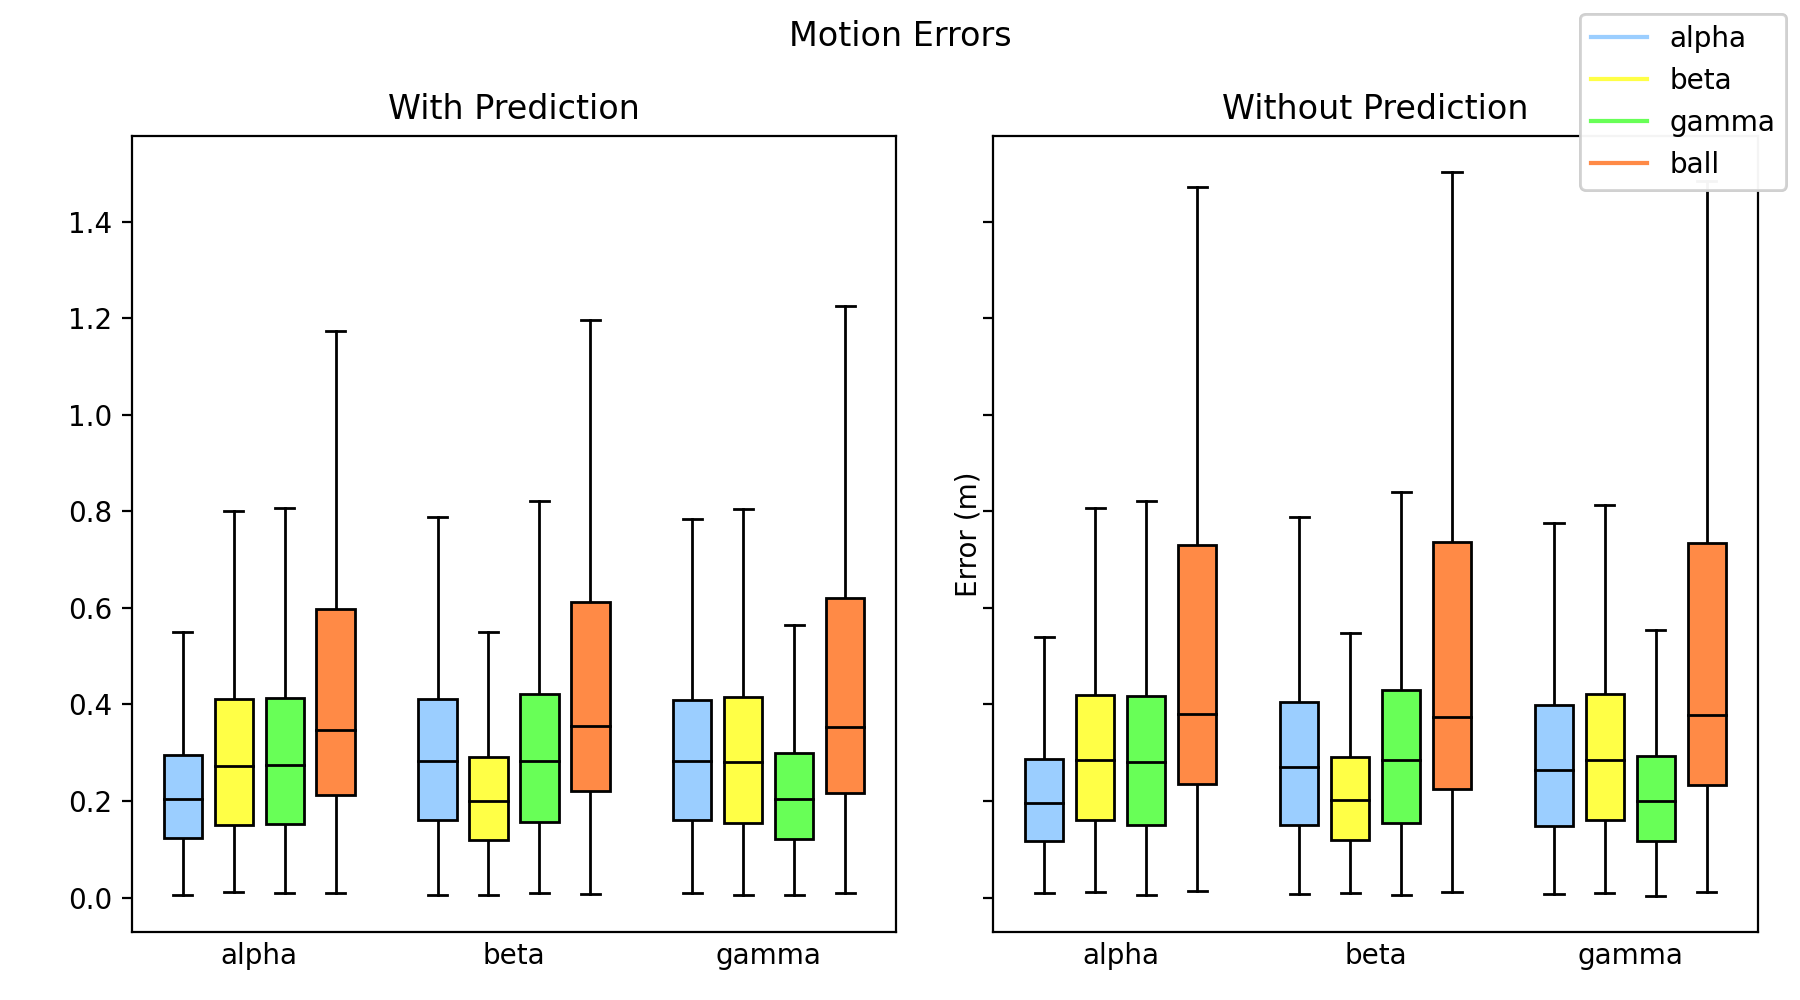
\includegraphics[width=0.9\textwidth]{resources/cfg1_AR_ARB_error_motion.png}
    \caption{\textit{Error} \textit{world model} R dan RB jaringan baik}
    \label{fig:1-r-rb-error}
    \bigskip
\end{figure}

Pada grafik \ref{fig:1-r-rb-error}, hasil estimasi posisi yang tidak dikompensasi cukup lebih buruk jika dibandingkan dengan estimasi dengan kompensasi waktu. Maka dapat dilihat kompensasi waktu dapat membantu untuk meningkatkan akurasi estimasi untuk objek seperti robot teman yang mungkin terlambat karena latensi atau bola yang mungkin tidak dipersepsi atau datanya terlambat karena latensi.

\section{Pengujian dan Analisis Algoritma Estimasi Data Terlambat}

\subsection{Perbandingan Algoritma Estimasi Bola Menggunakan PF dan OOSM-PF}

Dibandingkan dengan \textit{world model} R, \textit{world model} S menggunakan modifikasi OOSM-PF untuk dapat mengintegrasi data bola teman yang terlambat, daripada dengan PF biasa.

\begin{figure}[p]
    \centering
    \medskip
    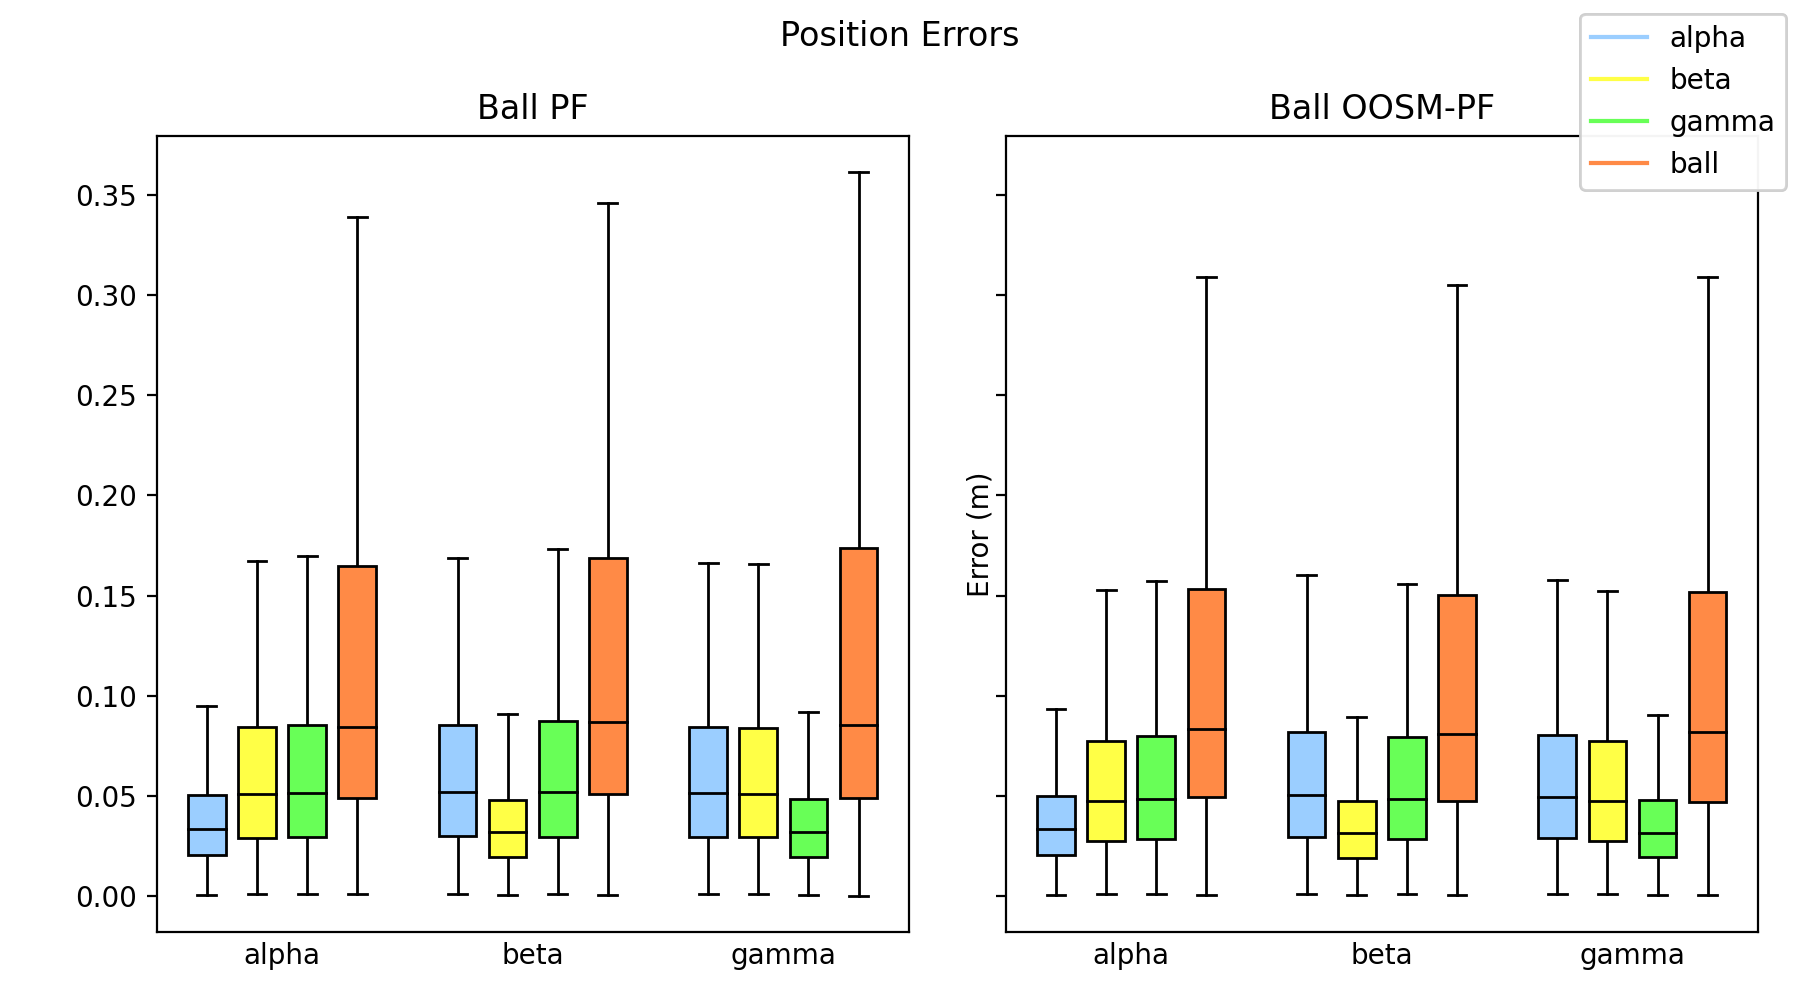
\includegraphics[width=0.9\textwidth]{resources/cfg1_AR_AS_error_pos.png}
    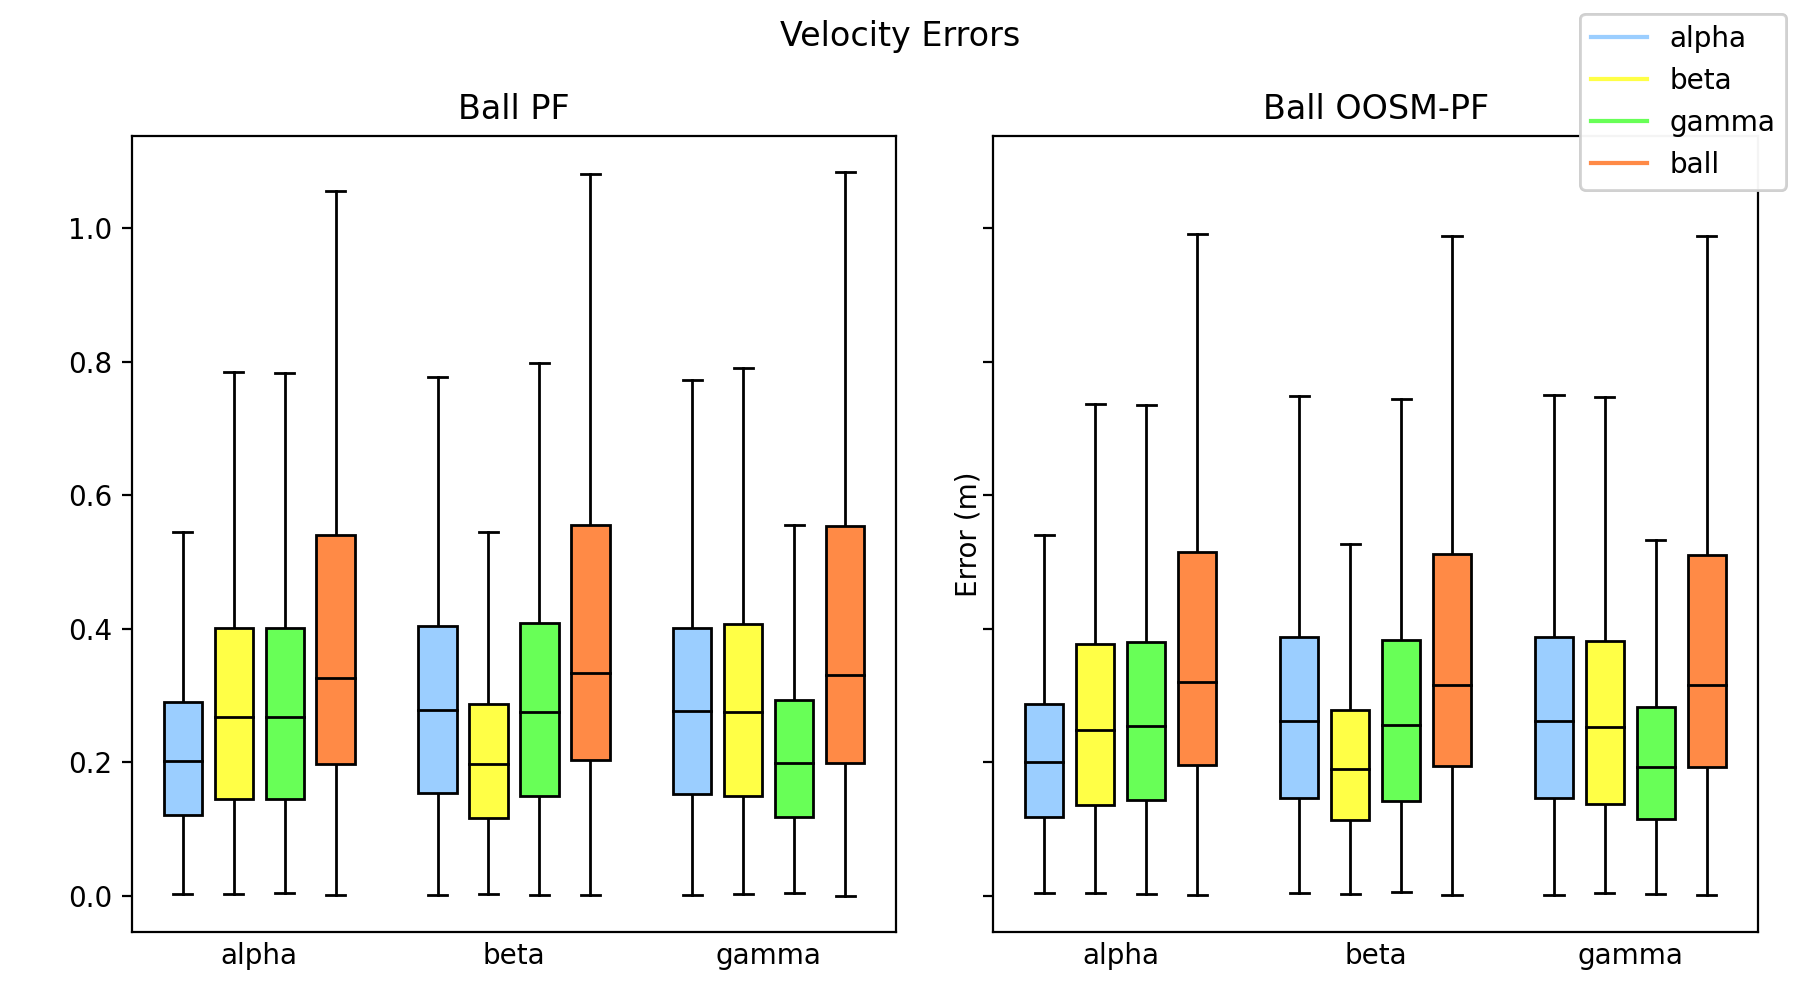
\includegraphics[width=0.9\textwidth]{resources/cfg1_AR_AS_error_vel.png}
    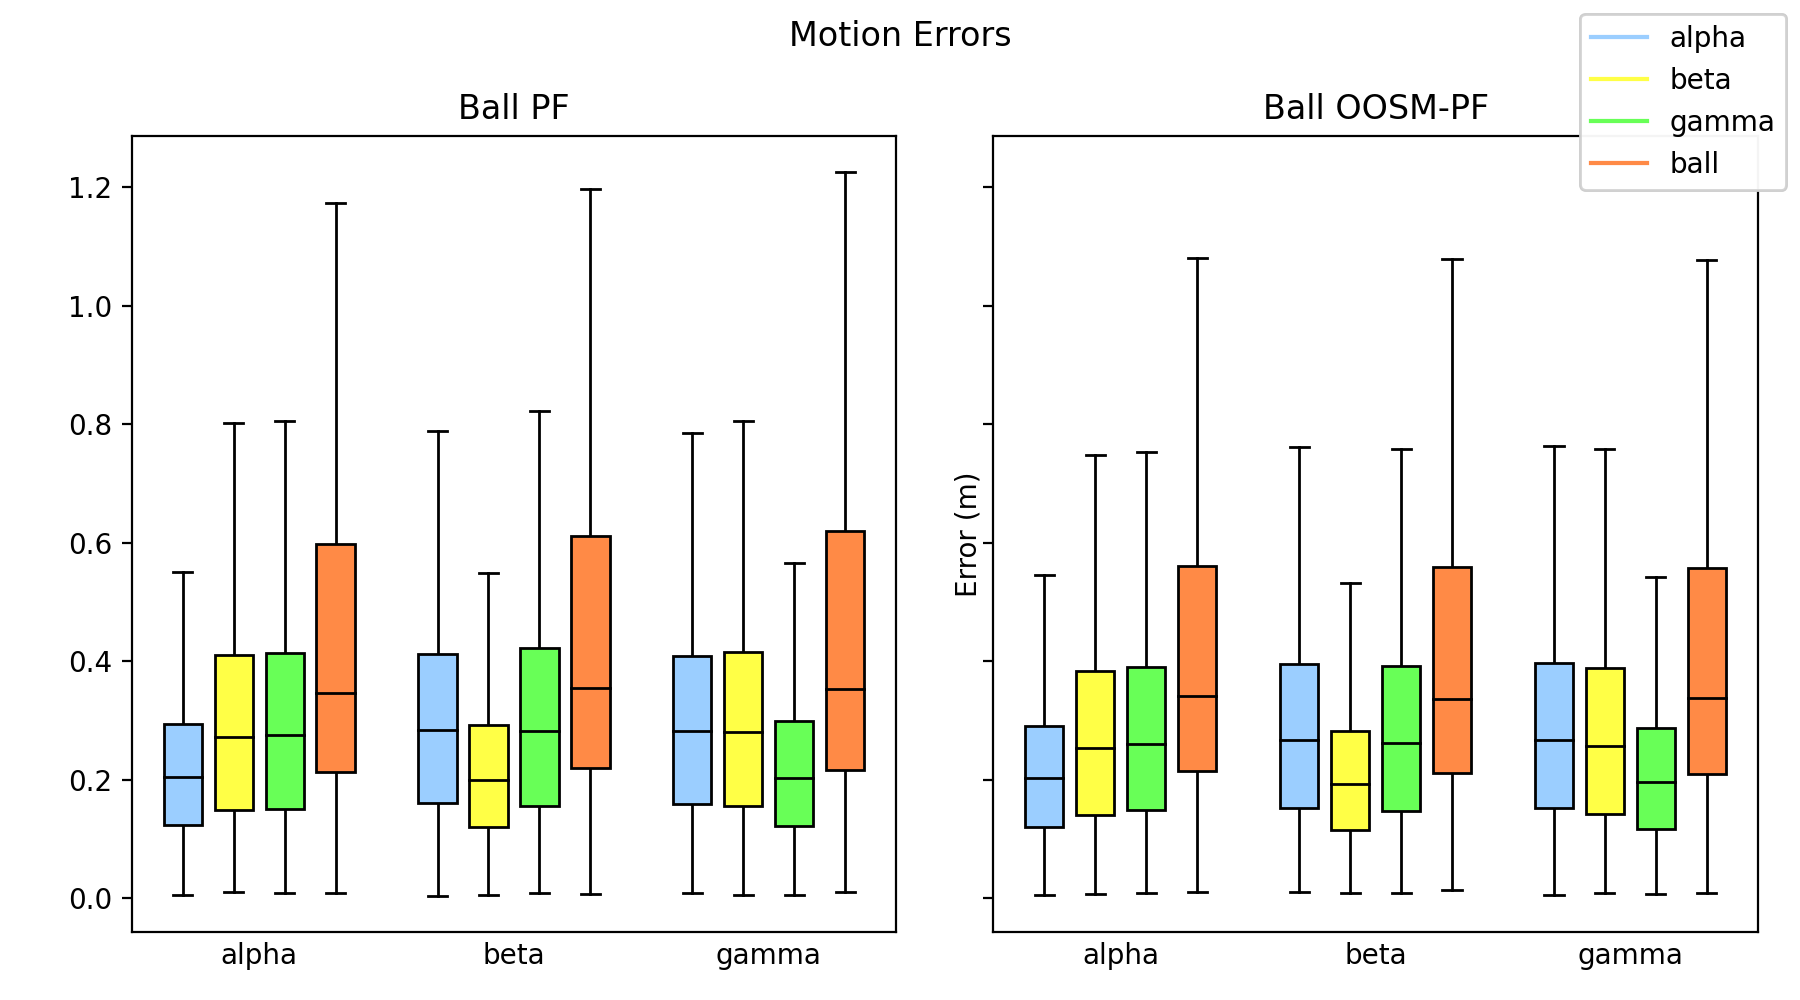
\includegraphics[width=0.9\textwidth]{resources/cfg1_AR_AS_error_motion.png}
    \caption{\textit{Error} \textit{world model} R dan S jaringan baik}
    \label{fig:1-r-s-error}
    \bigskip
\end{figure}

\begin{figure}[p]
    \centering
    \medskip
    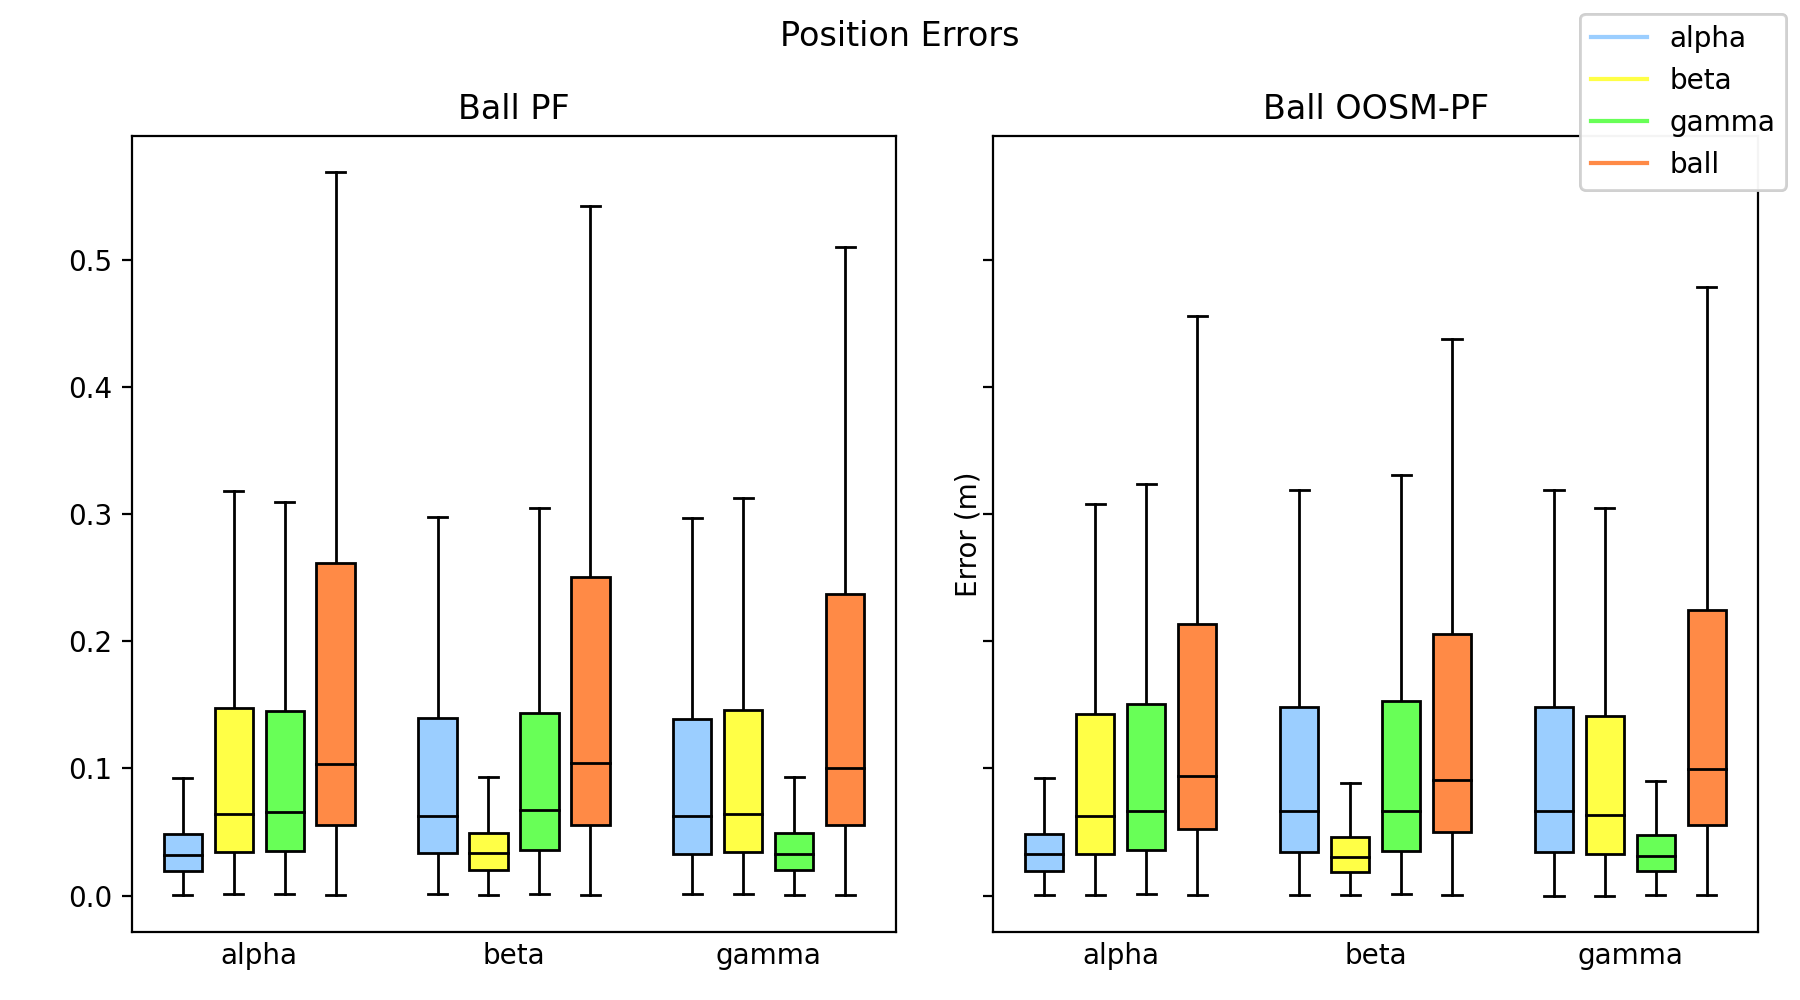
\includegraphics[width=0.9\textwidth]{resources/cfg2_AR_AS_error_pos.png}
    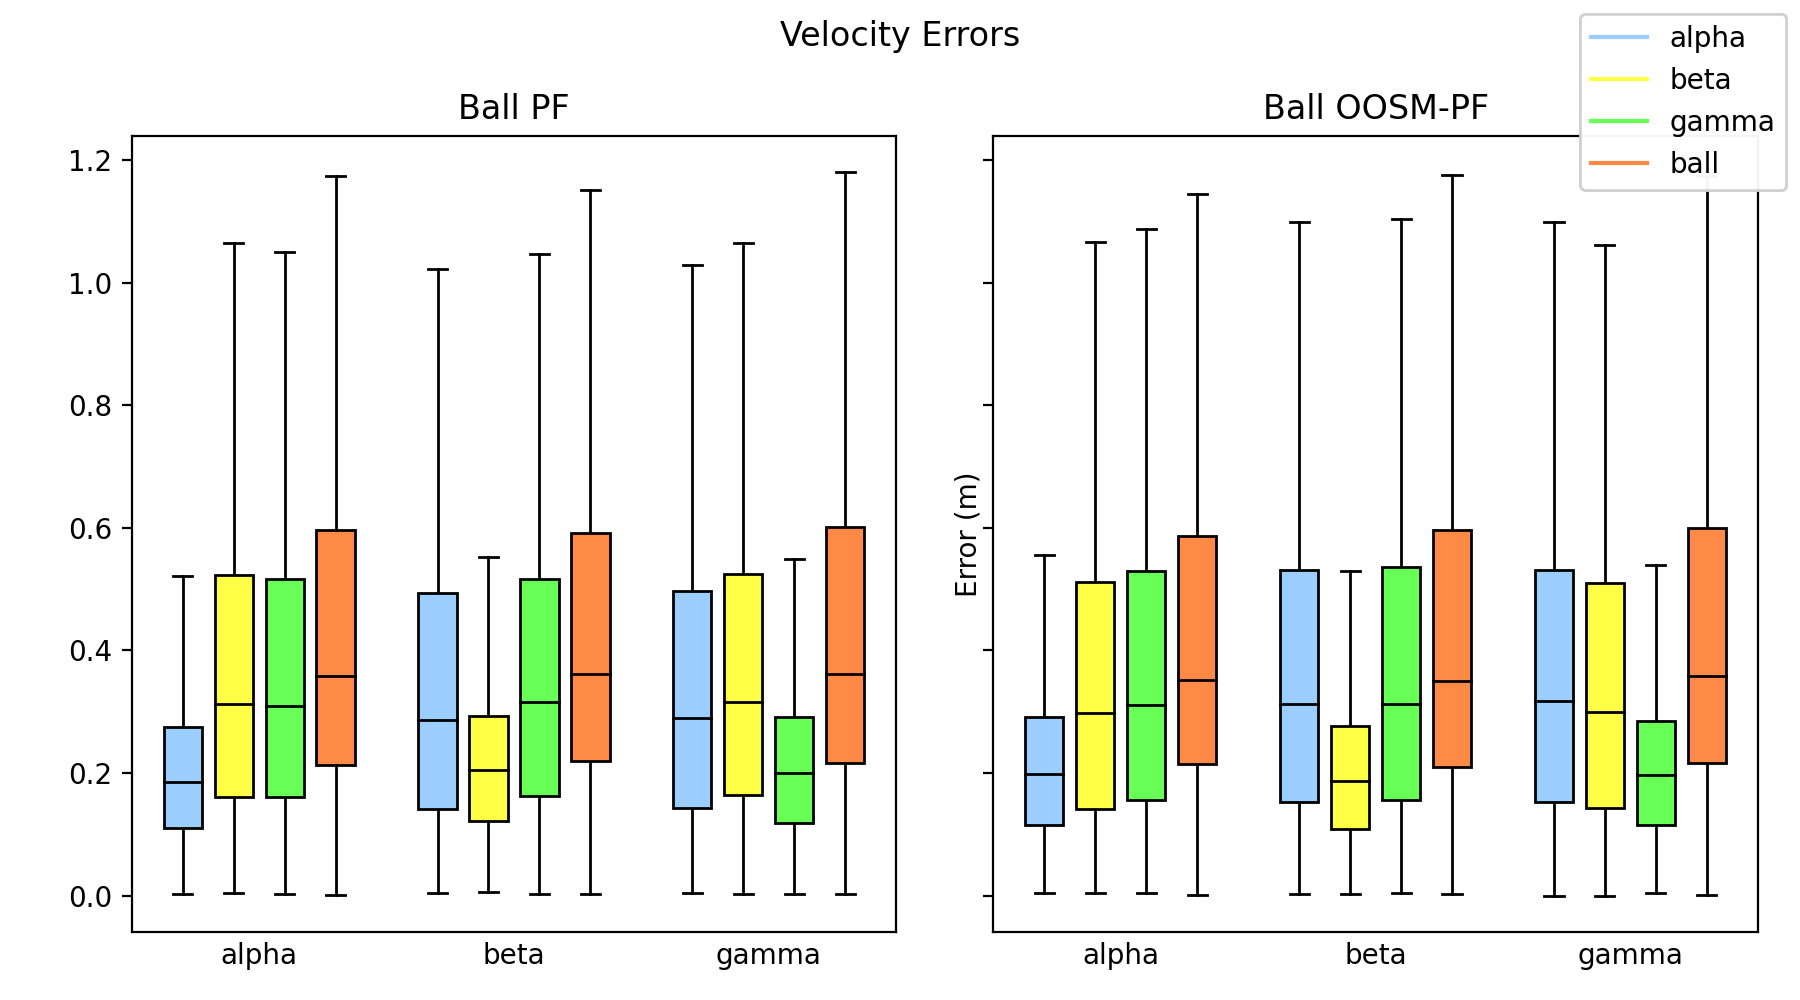
\includegraphics[width=0.9\textwidth]{resources/cfg2_AR_AS_error_vel.png}
    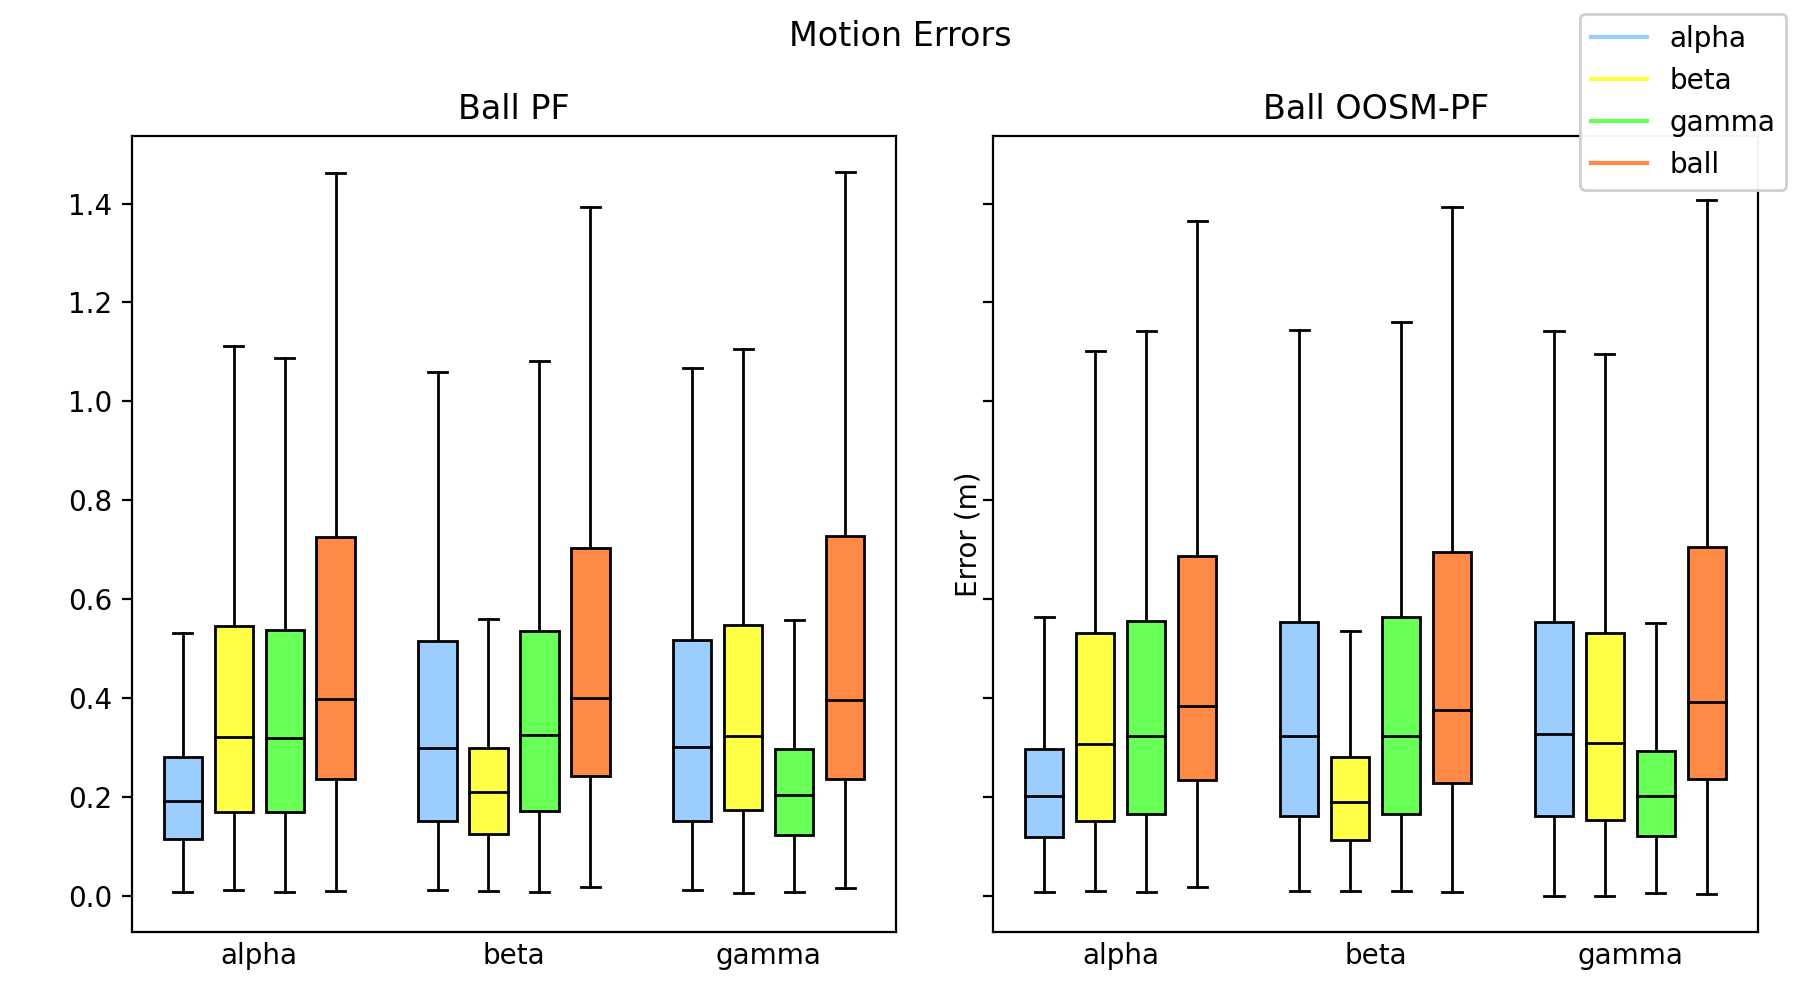
\includegraphics[width=0.9\textwidth]{resources/cfg2_AR_AS_error_motion.png}
    \caption{\textit{Error} \textit{world model} R dan S jaringan sedang}
    \label{fig:2-r-s-error}
    \bigskip
\end{figure}

\begin{figure}[p]
    \centering
    \medskip
    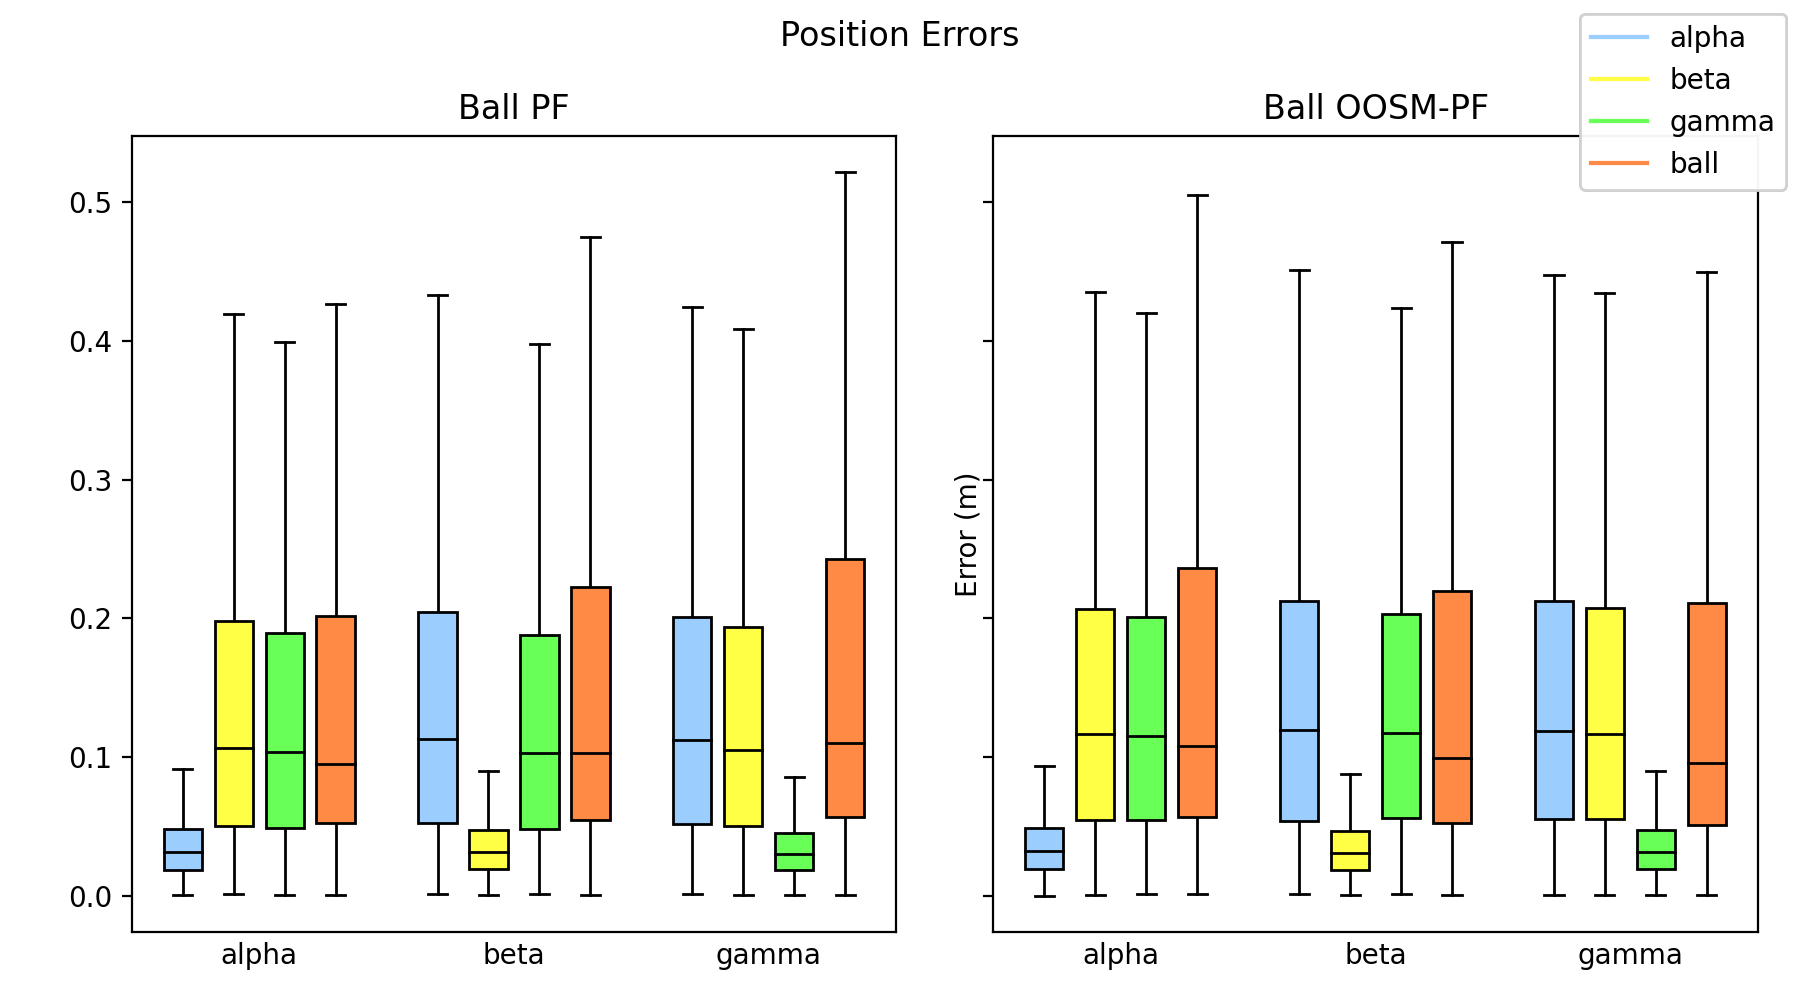
\includegraphics[width=0.9\textwidth]{resources/cfg3_AR_AS_error_pos.png}
    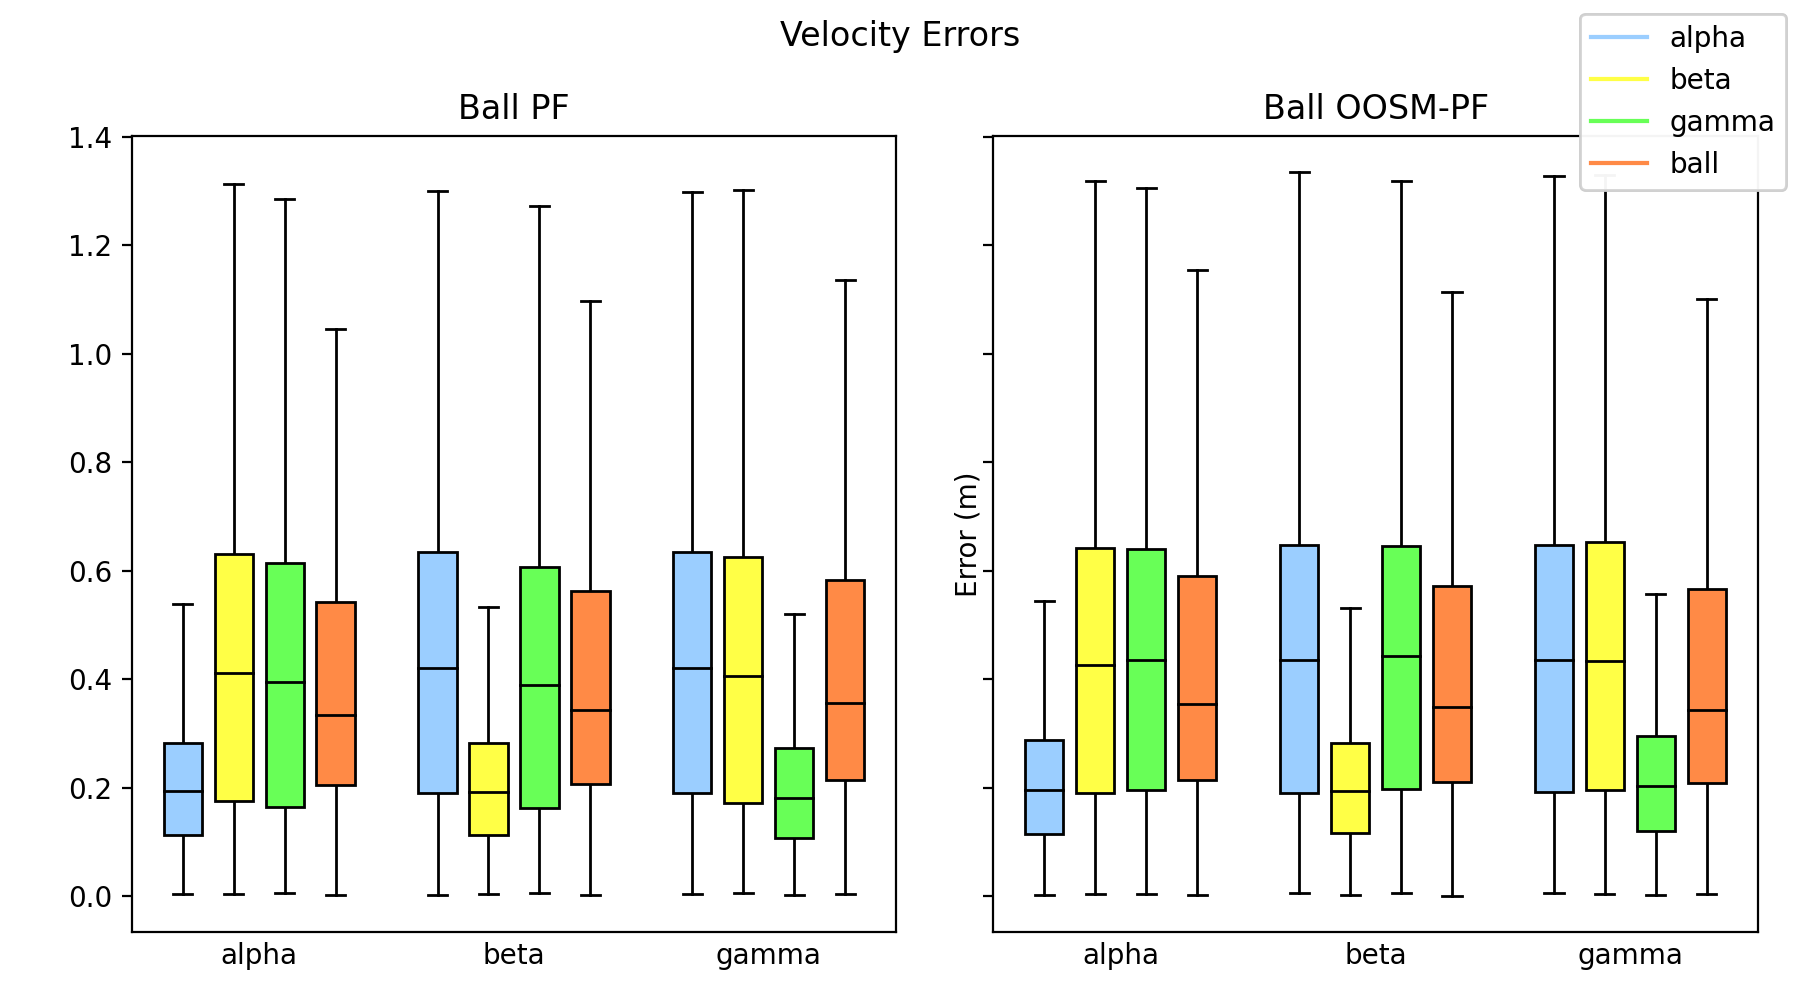
\includegraphics[width=0.9\textwidth]{resources/cfg3_AR_AS_error_vel.png}
    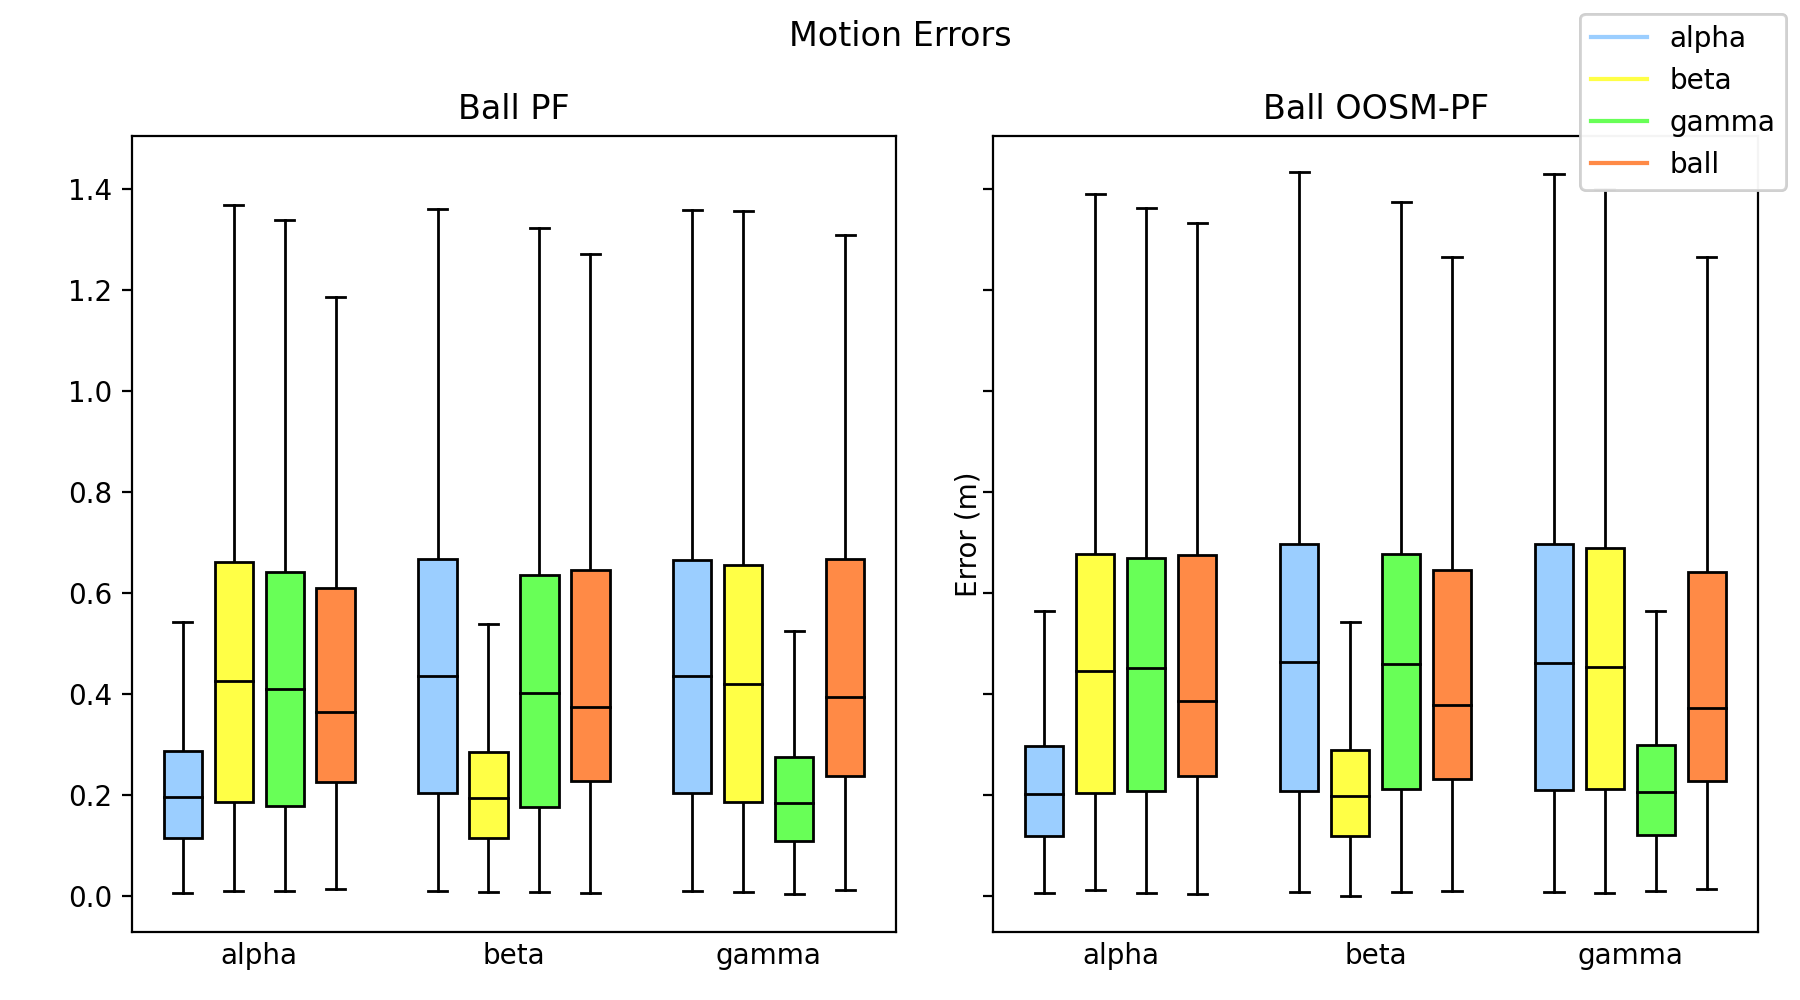
\includegraphics[width=0.9\textwidth]{resources/cfg3_AR_AS_error_motion.png}
    \caption{\textit{Error} \textit{world model} R dan S jaringan buruk}
    \label{fig:3-r-s-error}
    \bigskip
\end{figure}

Pada grafik \ref{fig:1-r-s-error}, terdapat peningkatan pada hasil estimasi posisi bola pada \textit{world model} yang menggunakan OOSM-PF saat jaringan baik, karena robot dapat mengintegrasi bacaan dari dua atau lebih robot yang melihat bola pada saat yang bersamaan untuk meningkatkan banyak data yang diintegrasi dan meningkatkan akurasi. Pada grafik \ref{fig:2-r-s-error} dan \ref{fig:3-r-s-error}, peningkatan ini semakin berkurang, karena pada saat robot dapat mengintegrasi data bola yang bersamaan dari dua robot atau lebih, data tersebut sudah cukup lama dan tidak lagi terlalu relevan terhadap hasil yang diestimasi sekarang.

\subsection{Perbandingan Algoritma Estimasi Bola tanpa Data Opsional dan dengan Data Opsional}

Dibandingkan dengan \textit{world model} S, \textit{world model} SB menggunakan OOSM-PF yang menerima data sensor yang dapat tidak melihat bola, daripada harus mengandung data bola yang terlihat.

\begin{figure}[p]
    \centering
    \medskip
    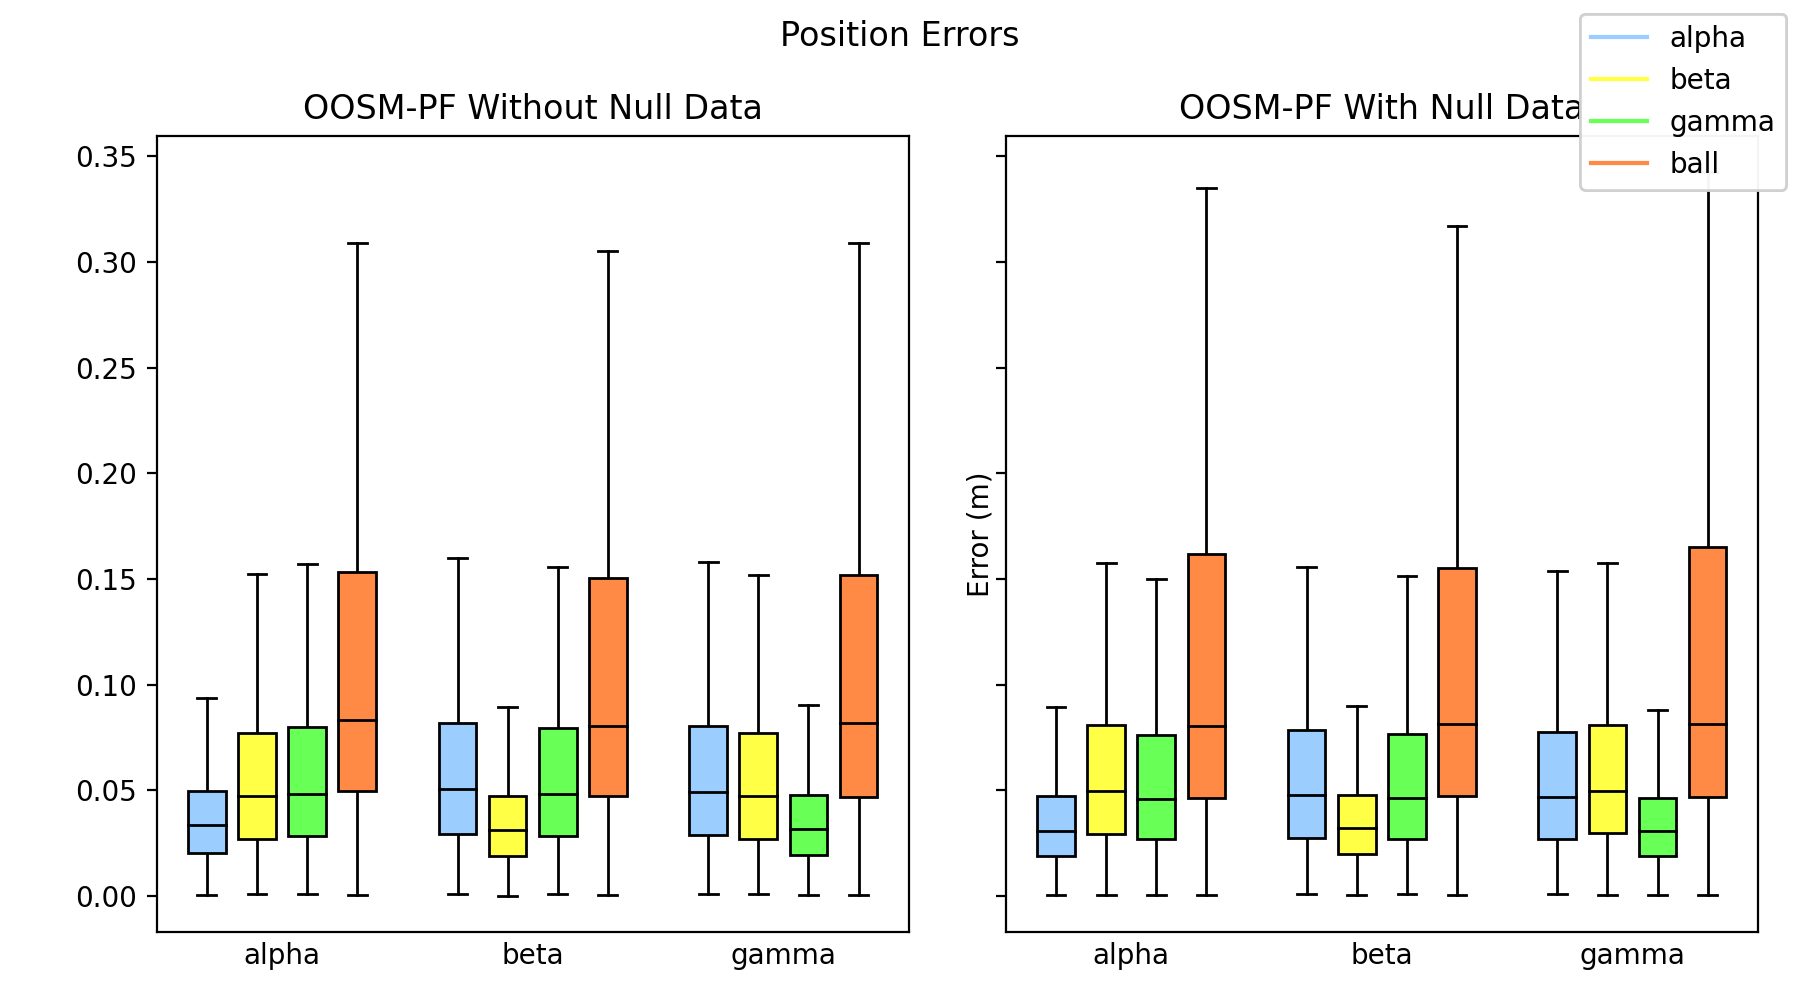
\includegraphics[width=0.9\textwidth]{resources/cfg1_AS_ASB_error_pos.png}
    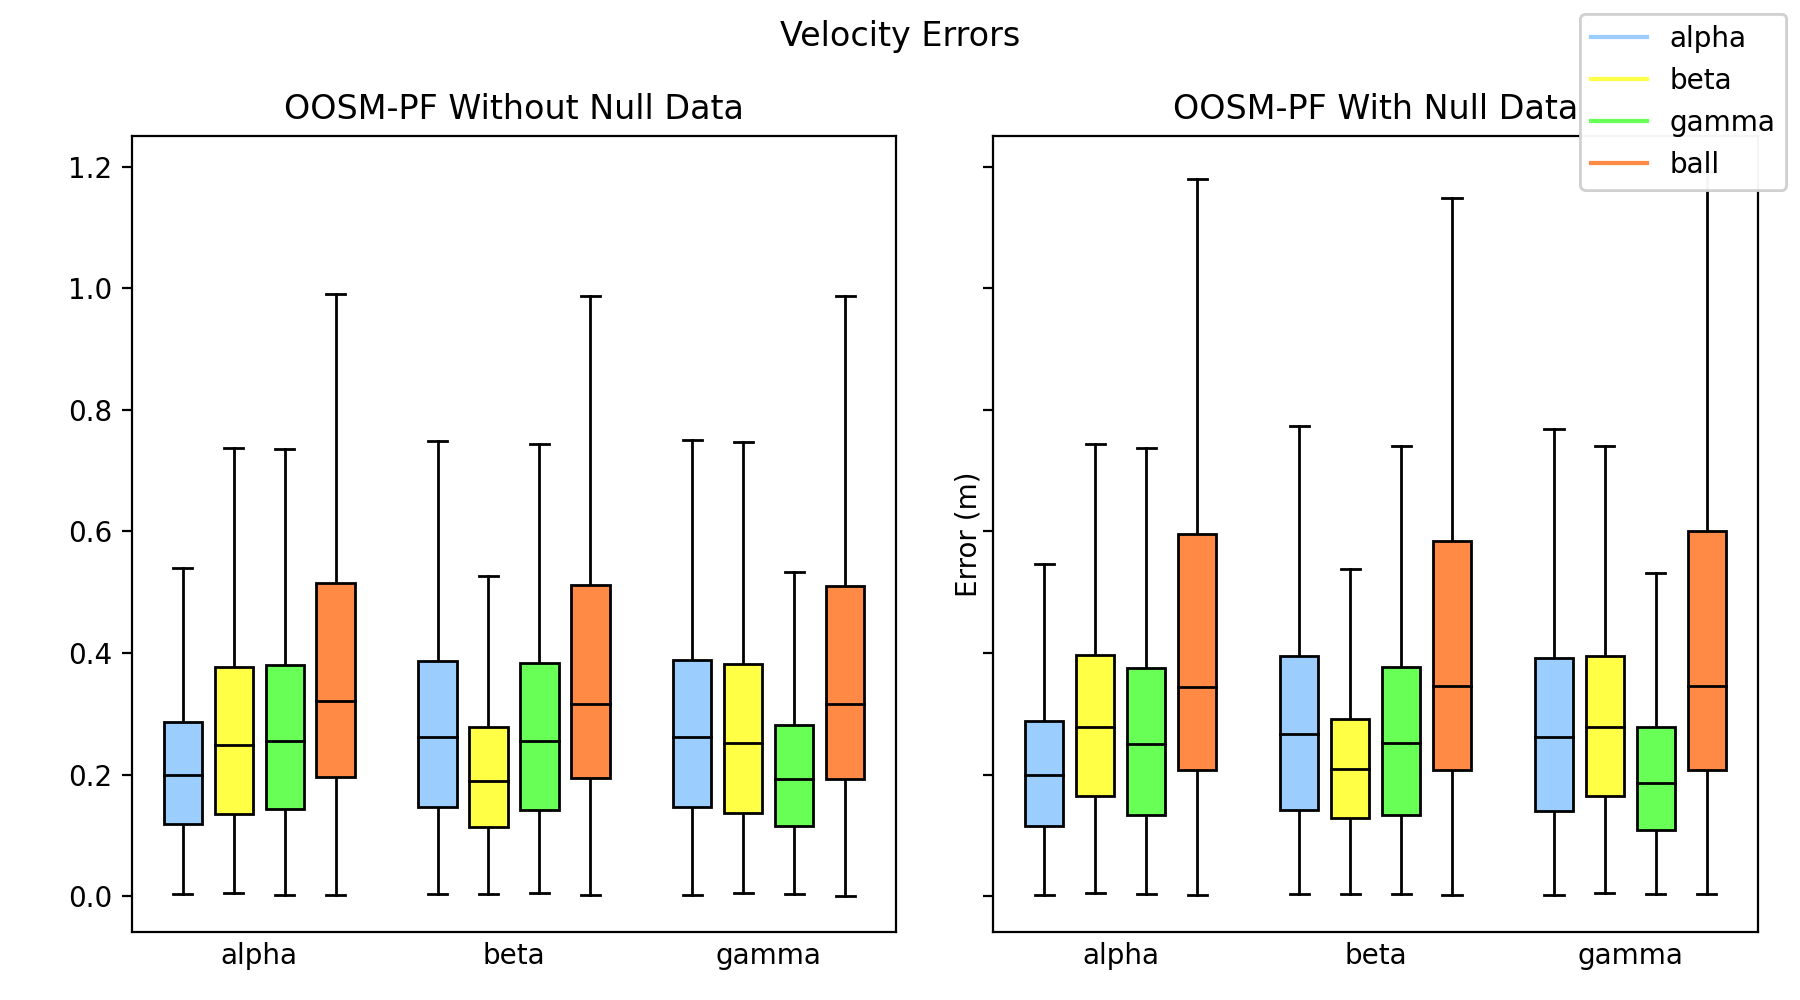
\includegraphics[width=0.9\textwidth]{resources/cfg1_AS_ASB_error_vel.png}
    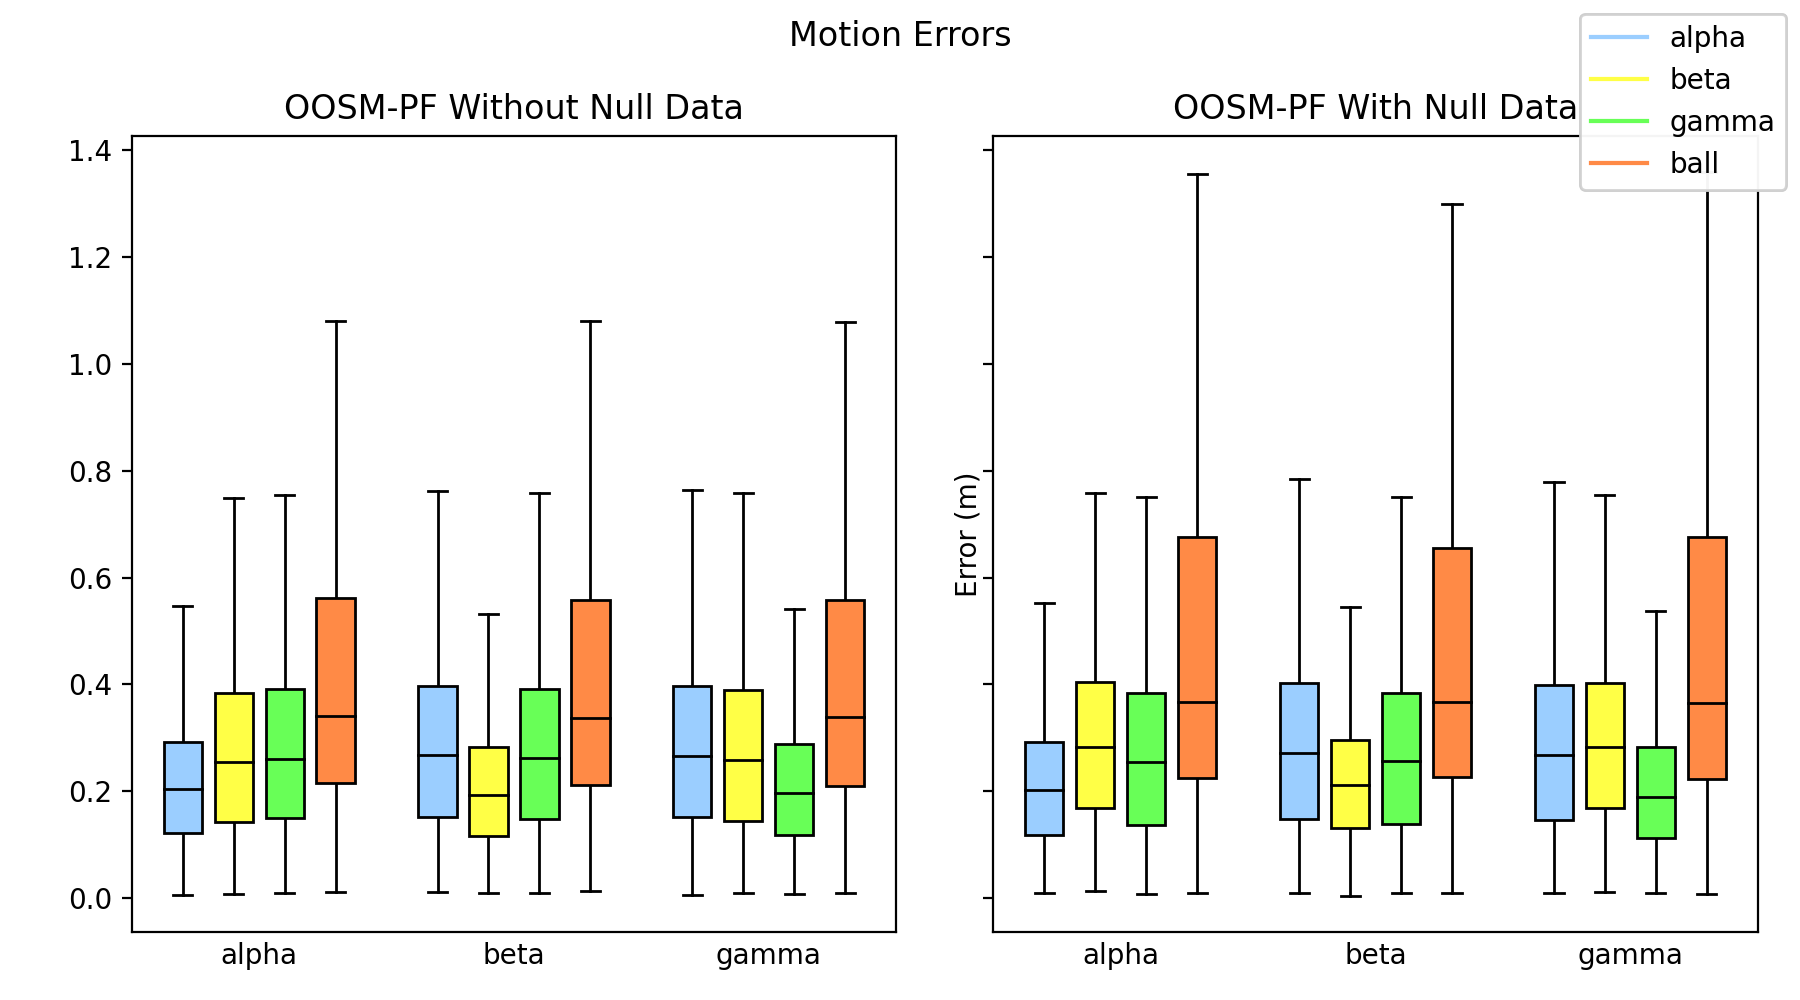
\includegraphics[width=0.9\textwidth]{resources/cfg1_AS_ASB_error_motion.png}
    \caption{\textit{Error} \textit{world model} S dan SB jaringan baik}
    \label{fig:1-s-sb-error}
    \bigskip
\end{figure}

Pada grafik \ref{fig:1-s-sb-error}, tidak ada perubahan yang signifikan dari integrasi data yang tidak \textit{null} untuk estimasi posisi dan malah memburuk untuk hasil estimasi kecepatan. Ini tampaknya disebabkan karena algoritma ini tidak mempertimbangkan saat bola tidak terlihat karena oklusi dari objek, sehingga saat bola tidak terlihat, partikel yang ada di luar lingkaran radius penglihatan punya berat yang lebih tinggi dan punya kecenderungan memiliki kecepatan yang lebih tinggi dalam menjauhi robot keluar dari lingkaran.

\subsection{Perbandingan Algoritma Estimasi Bola dengan OOSM-PF dan OOSM-KF}

Dibandingkan dengan \textit{world model} S, \textit{world model} SC menggunakan OOSM-KF yang berdasarkan algoritma penapis Kalman, daripada algoritma OOSM-PF yang berdasarkan algoritma penapis partikel.

\begin{figure}[p]
    \centering
    \medskip
    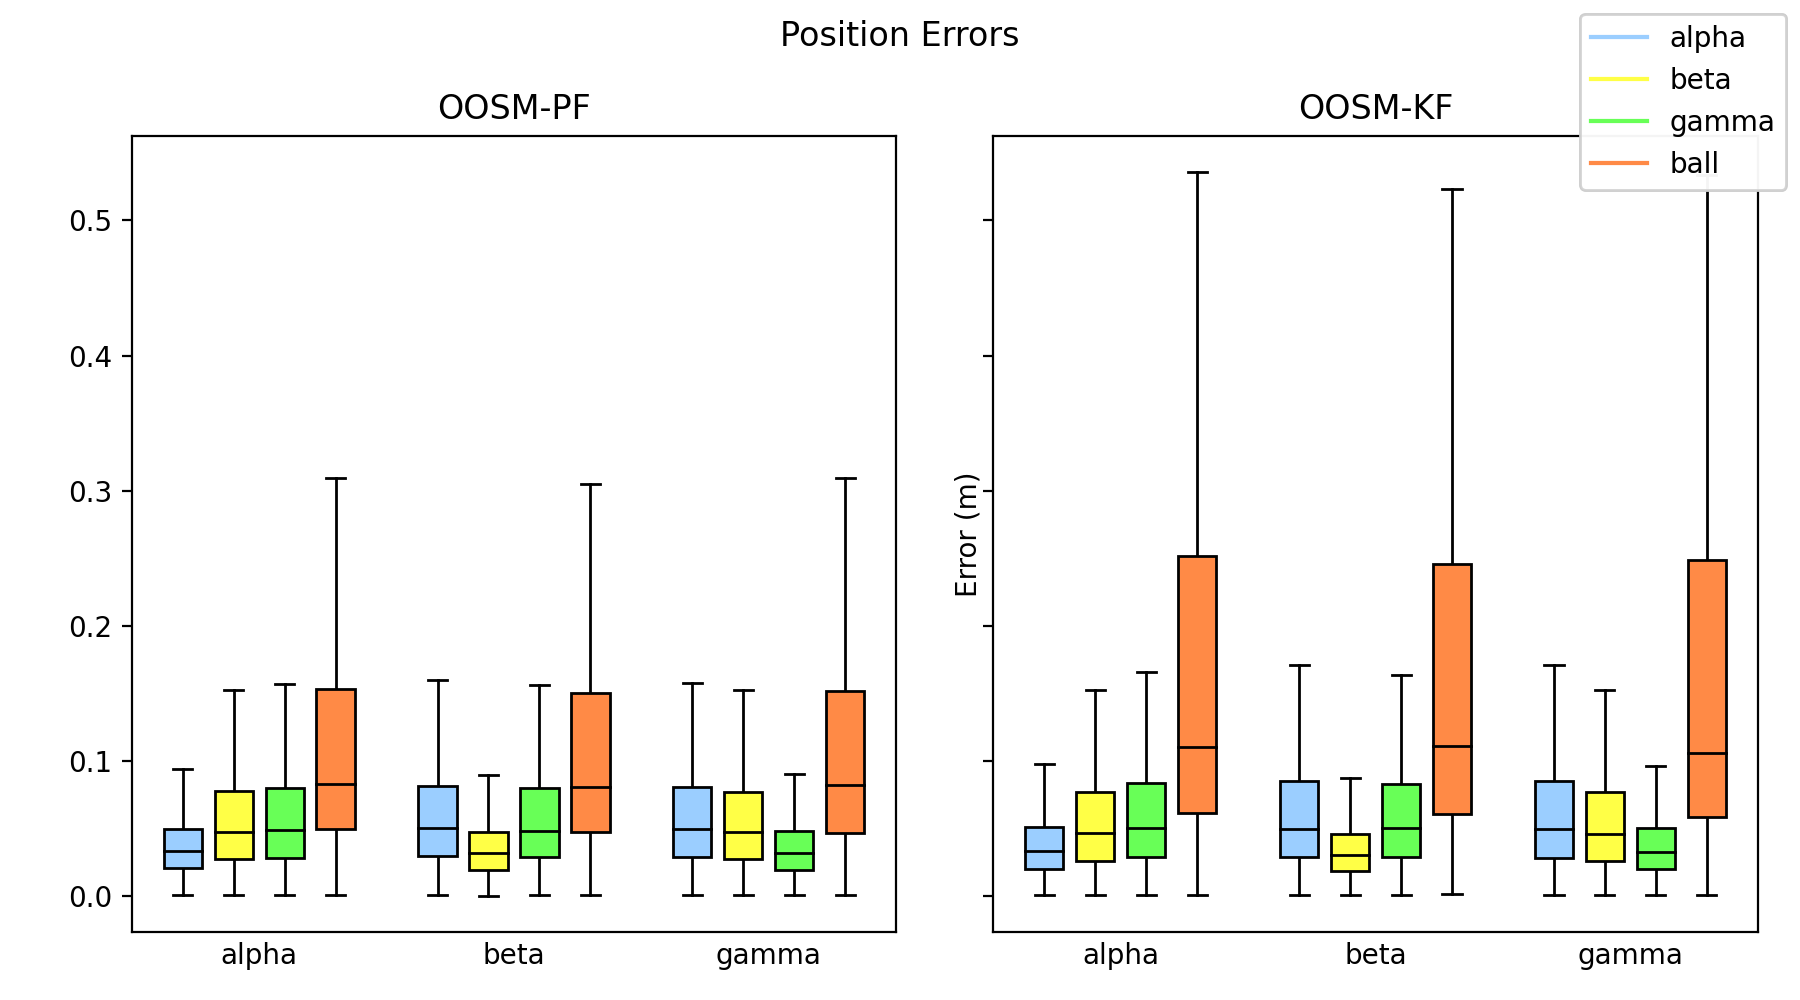
\includegraphics[width=0.9\textwidth]{resources/cfg1_AS_ASC_error_pos.png}
    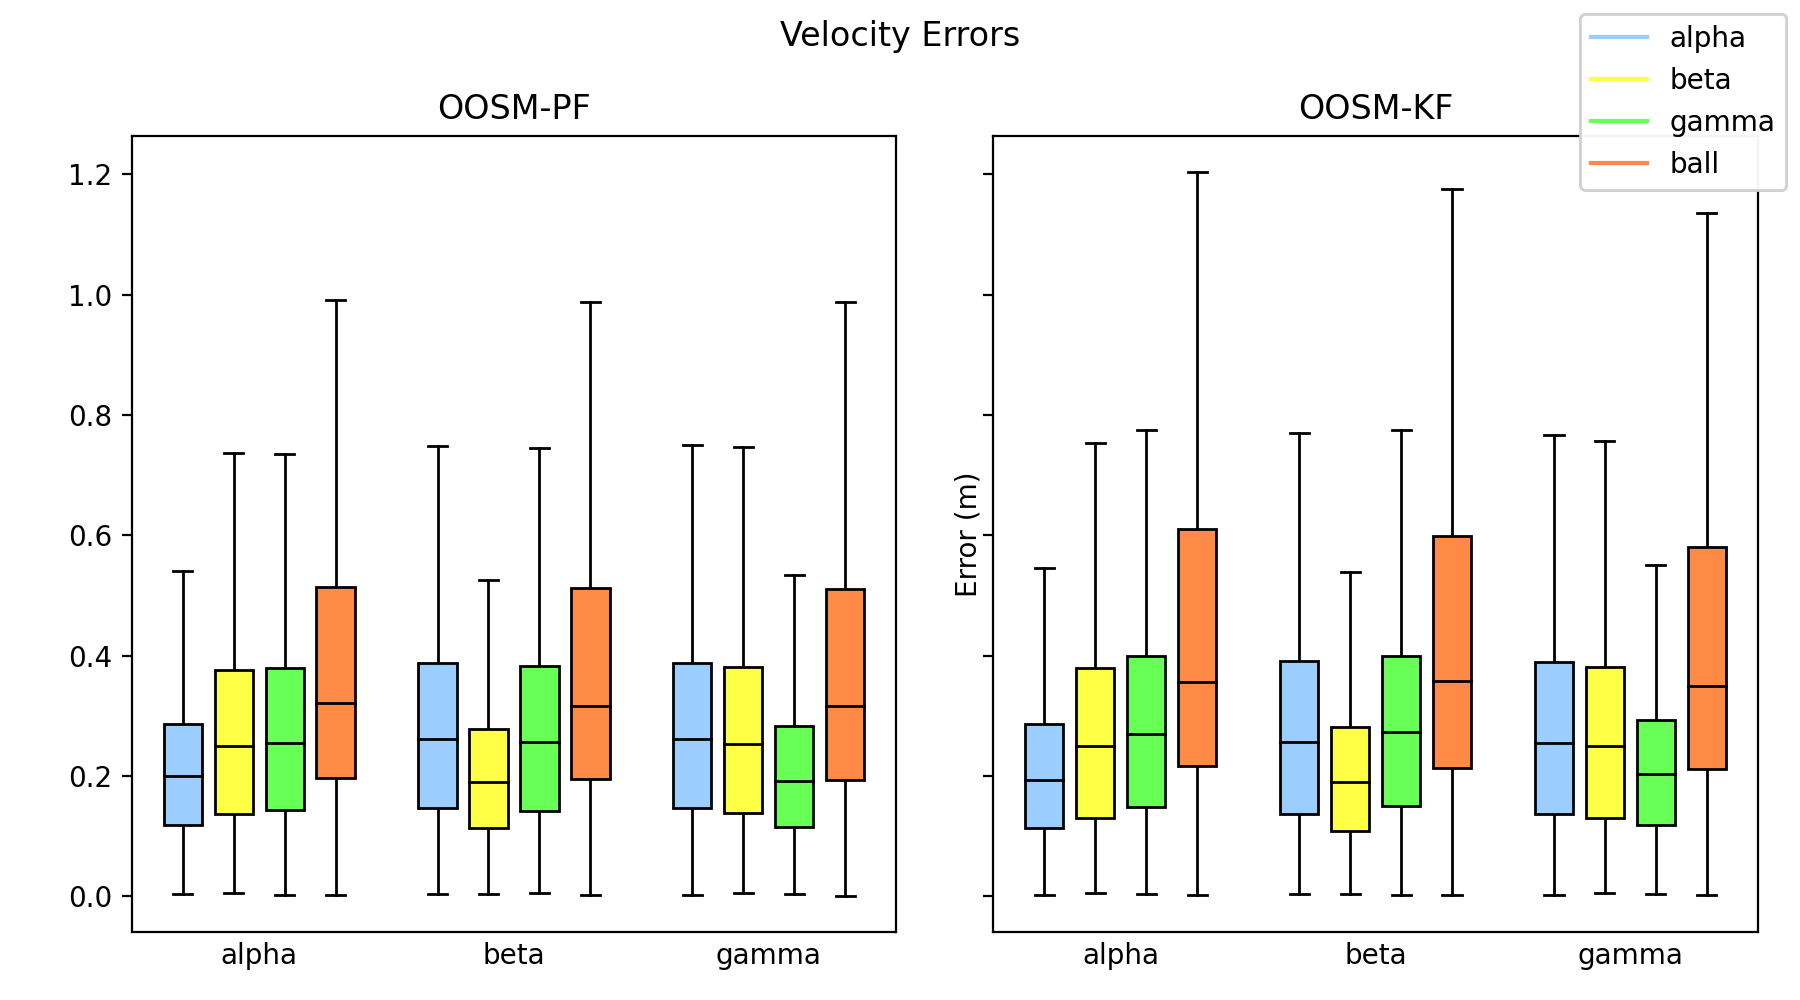
\includegraphics[width=0.9\textwidth]{resources/cfg1_AS_ASC_error_vel.png}
    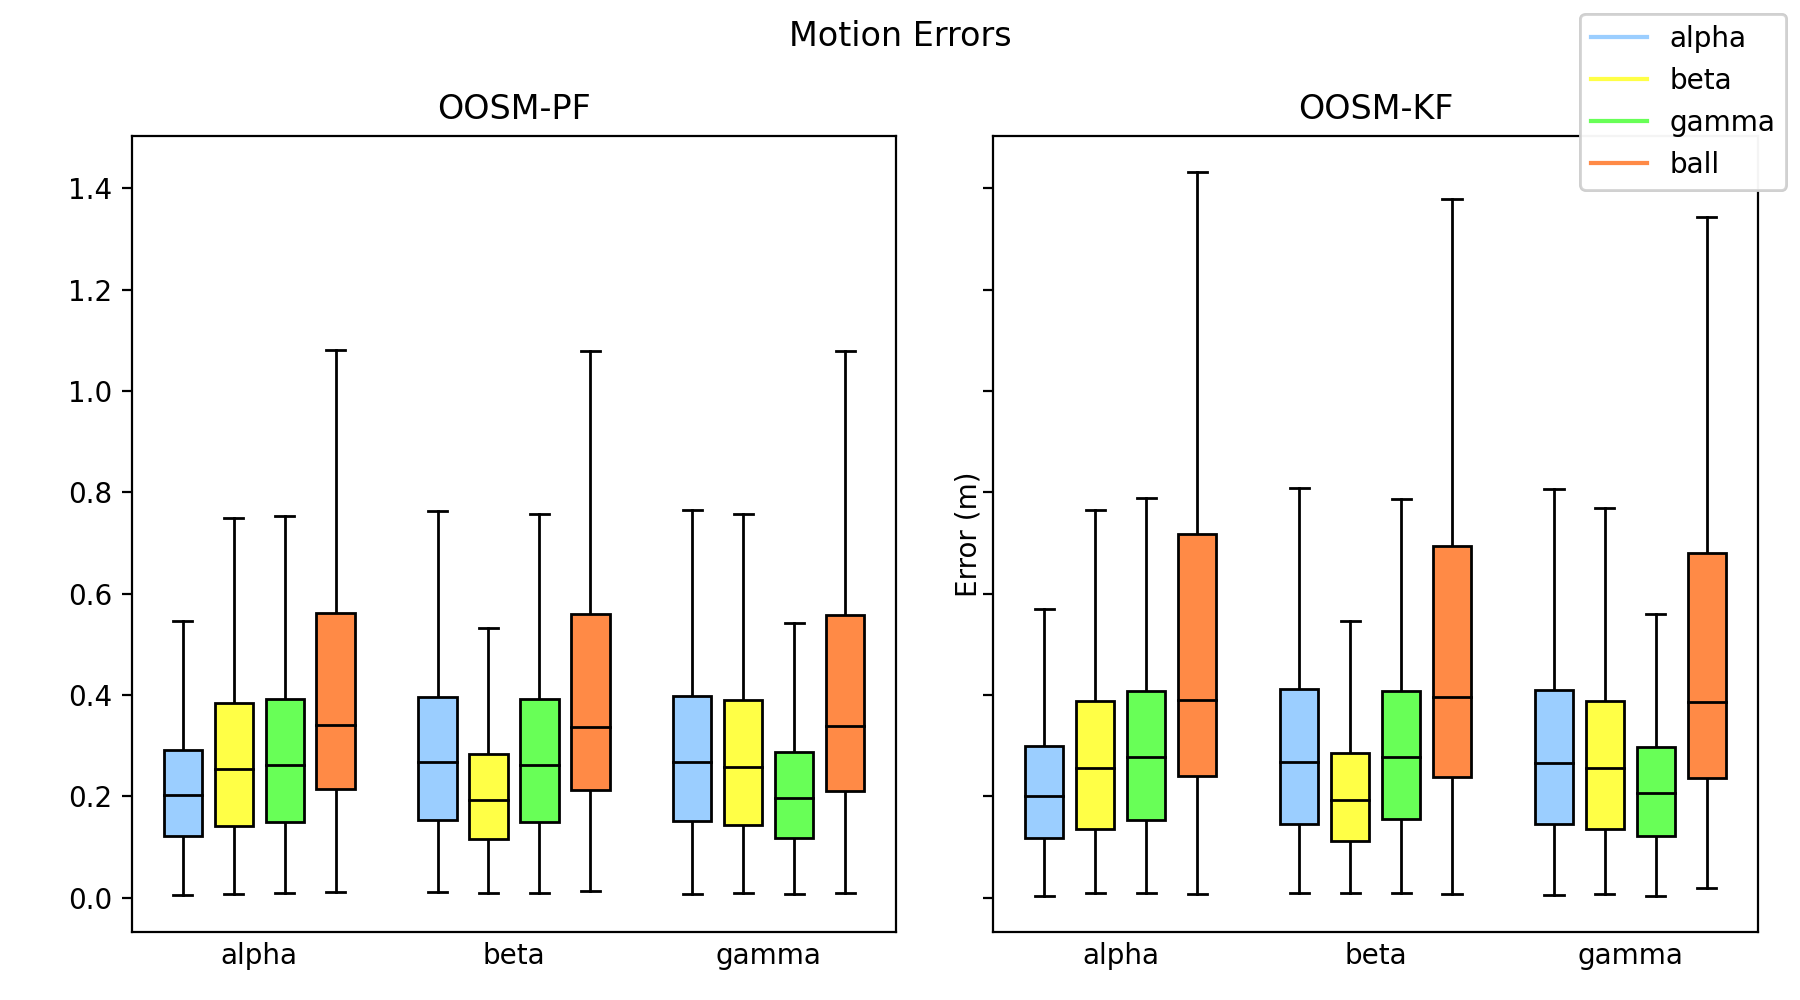
\includegraphics[width=0.9\textwidth]{resources/cfg1_AS_ASC_error_motion.png}
    \caption{\textit{Error} \textit{world model} S dan SC jaringan baik}
    \label{fig:1-s-sc-error}
    \bigskip
\end{figure}

Pada grafik \ref{fig:1-s-sc-error}, didapatkan \textit{error} estimasi posisi maupun kecepatan yang lebih buruk. Hal ini kemungkinan disebabkan oleh alasan yang sama dengan perbandingan kinerja PF dan KF dimana KF tidak dapat dengan sempurna memodelkan profil \textit{error} dari \textit{vision}, apalagi saat menggabungkan data dari sudut pandang dua atau lebih robot yang berbeda dengan arah distribusi \textit{error} yang berbeda juga.

\subsection{Perbandingan Algoritma Estimasi Bola OOSM-PF Biasa dan OOSM-KF dengan Kombinasi Data}

Dibandingkan dengan \textit{world model} S, \textit{world model} SD menggunakan OOSM-KF yang menggabungkan beberapa persepsi bola pada waktu yang sama dengan merata-ratakan posisinya.

\begin{figure}[p]
    \centering
    \medskip
    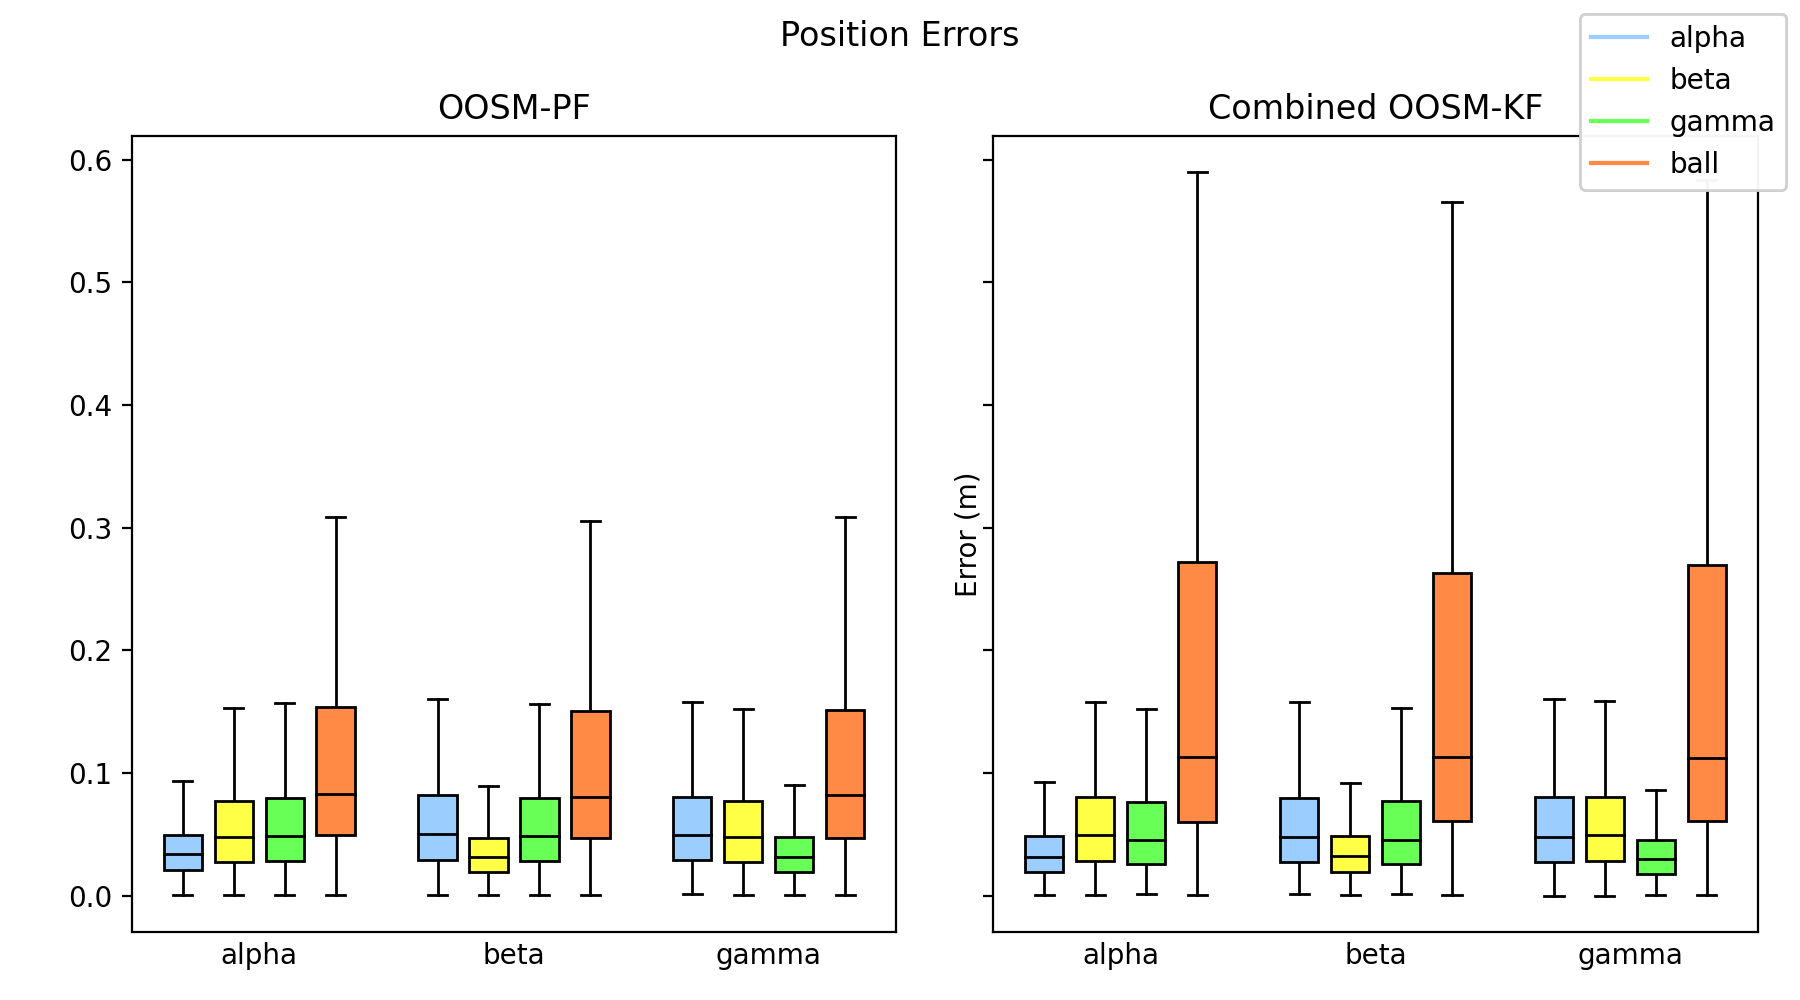
\includegraphics[width=0.9\textwidth]{resources/cfg1_AS_ASD_error_pos.png}
    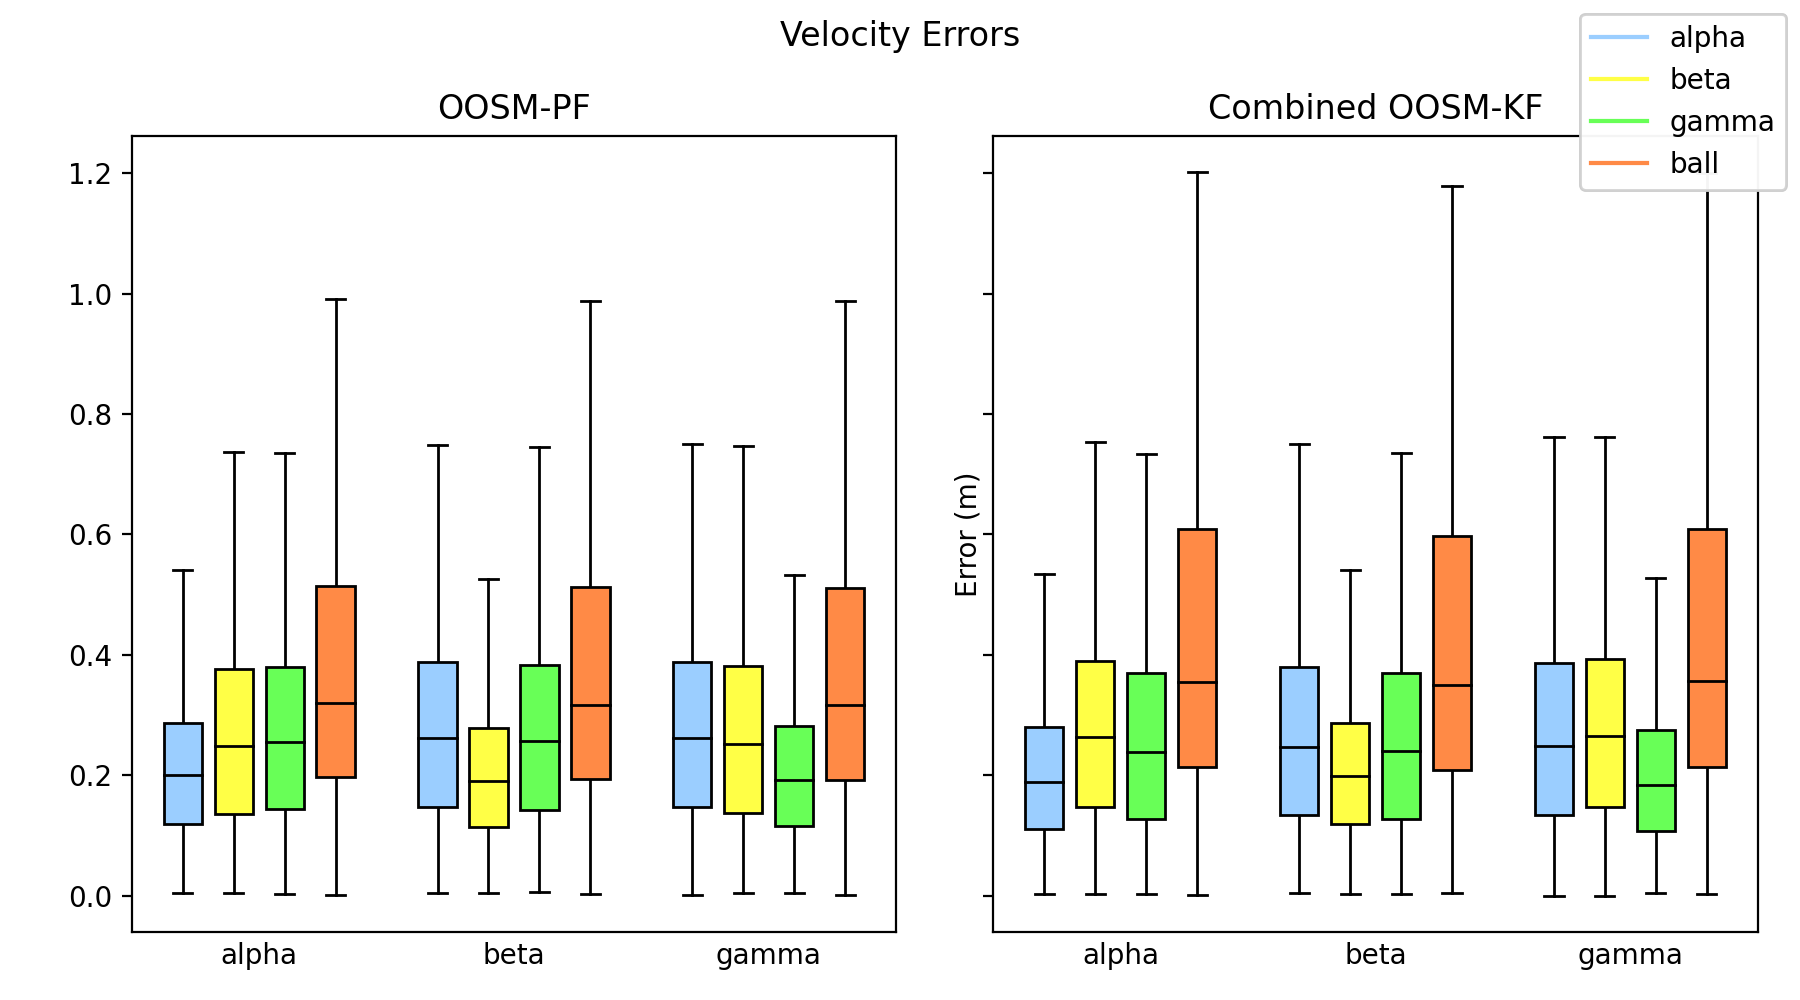
\includegraphics[width=0.9\textwidth]{resources/cfg1_AS_ASD_error_vel.png}
    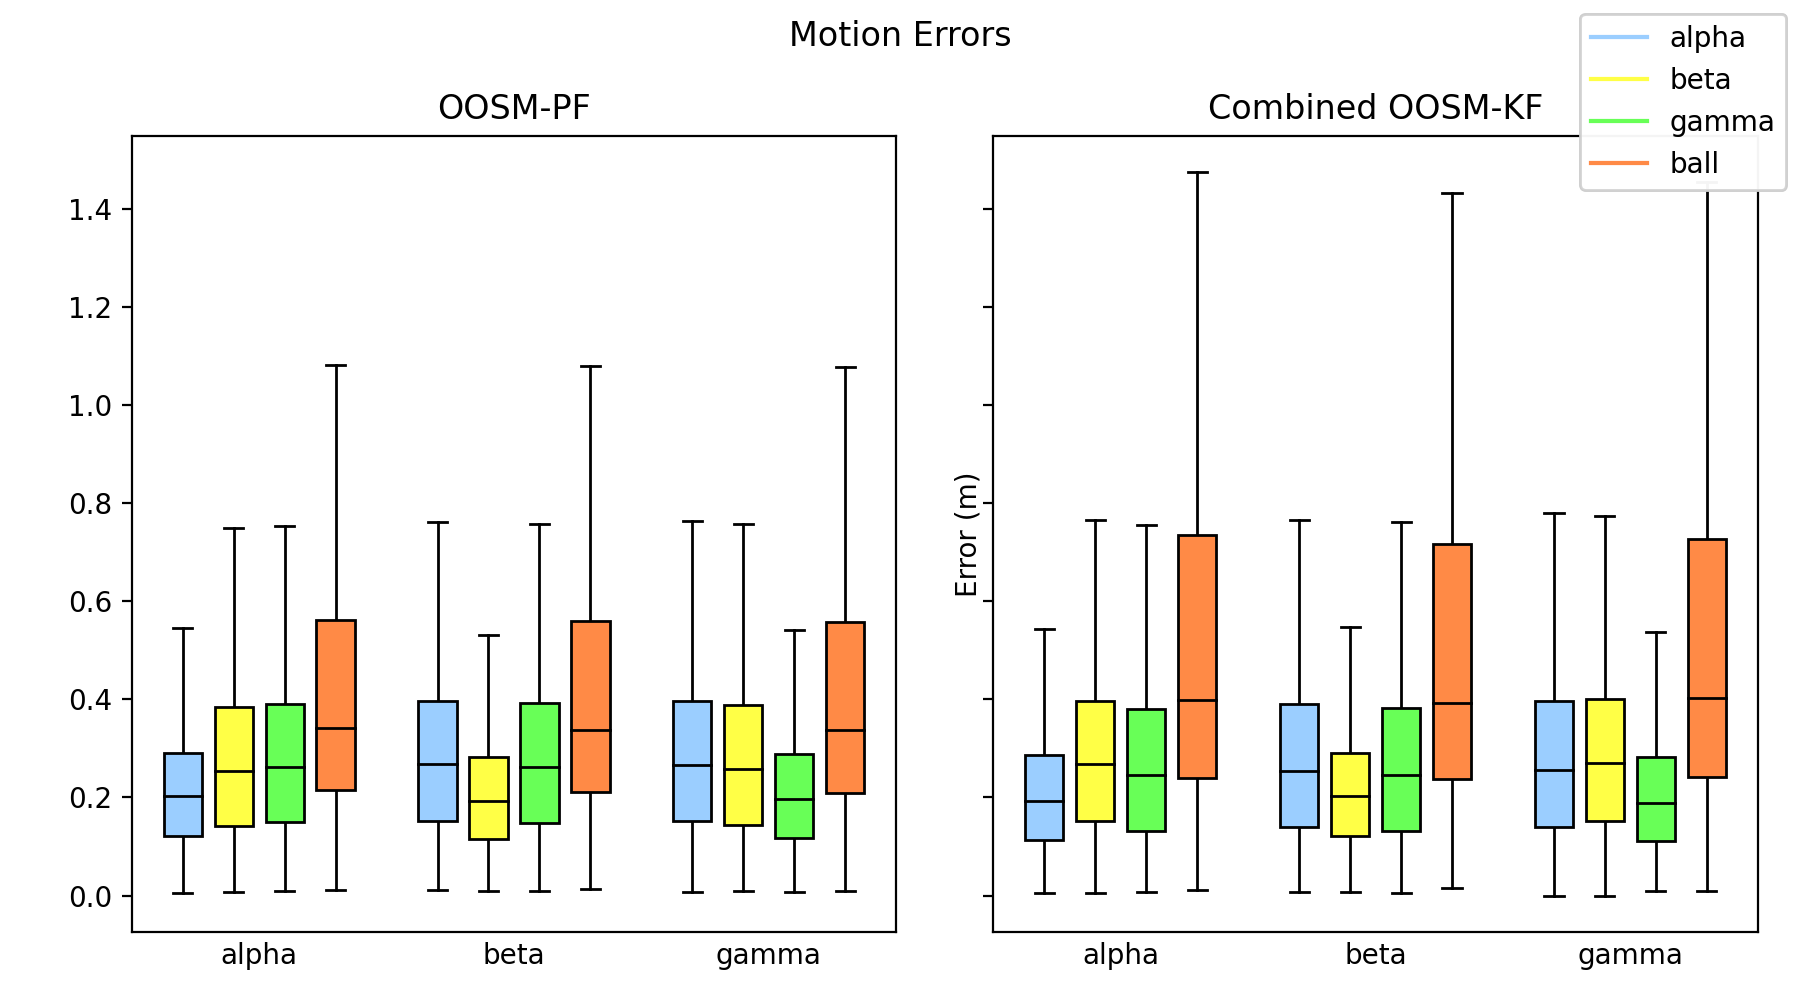
\includegraphics[width=0.9\textwidth]{resources/cfg1_AS_ASD_error_motion.png}
    \caption{\textit{Error} \textit{world model} S dan SD jaringan baik}
    \label{fig:1-s-sd-error}
    \bigskip
\end{figure}

Pada grafik \ref{fig:1-s-sd-error}, didapatkan \textit{error} estimasi posisi maupun kecepatan yang lebih buruk, dan kinerja \textit{world model} SD yang tidak jauh dari SC, yang kemungkinan dikarenakan oleh alasan yang sama dimana penggunaan OOSM-KFnya tidak cocok untuk profil \textit{error} \textit{vision} yang ada.

\subsection{Perbandingan Algoritma tanpa dan dengan Koreksi Posisi Robot Teman}

Dibandingkan dengan \textit{world model} S, \textit{world model} T mengoreksi posisi teman yang diterima dari komunikasi menggunakan persepsi sendiri dari \textit{vision}.

\begin{figure}[p]
    \centering
    \medskip
    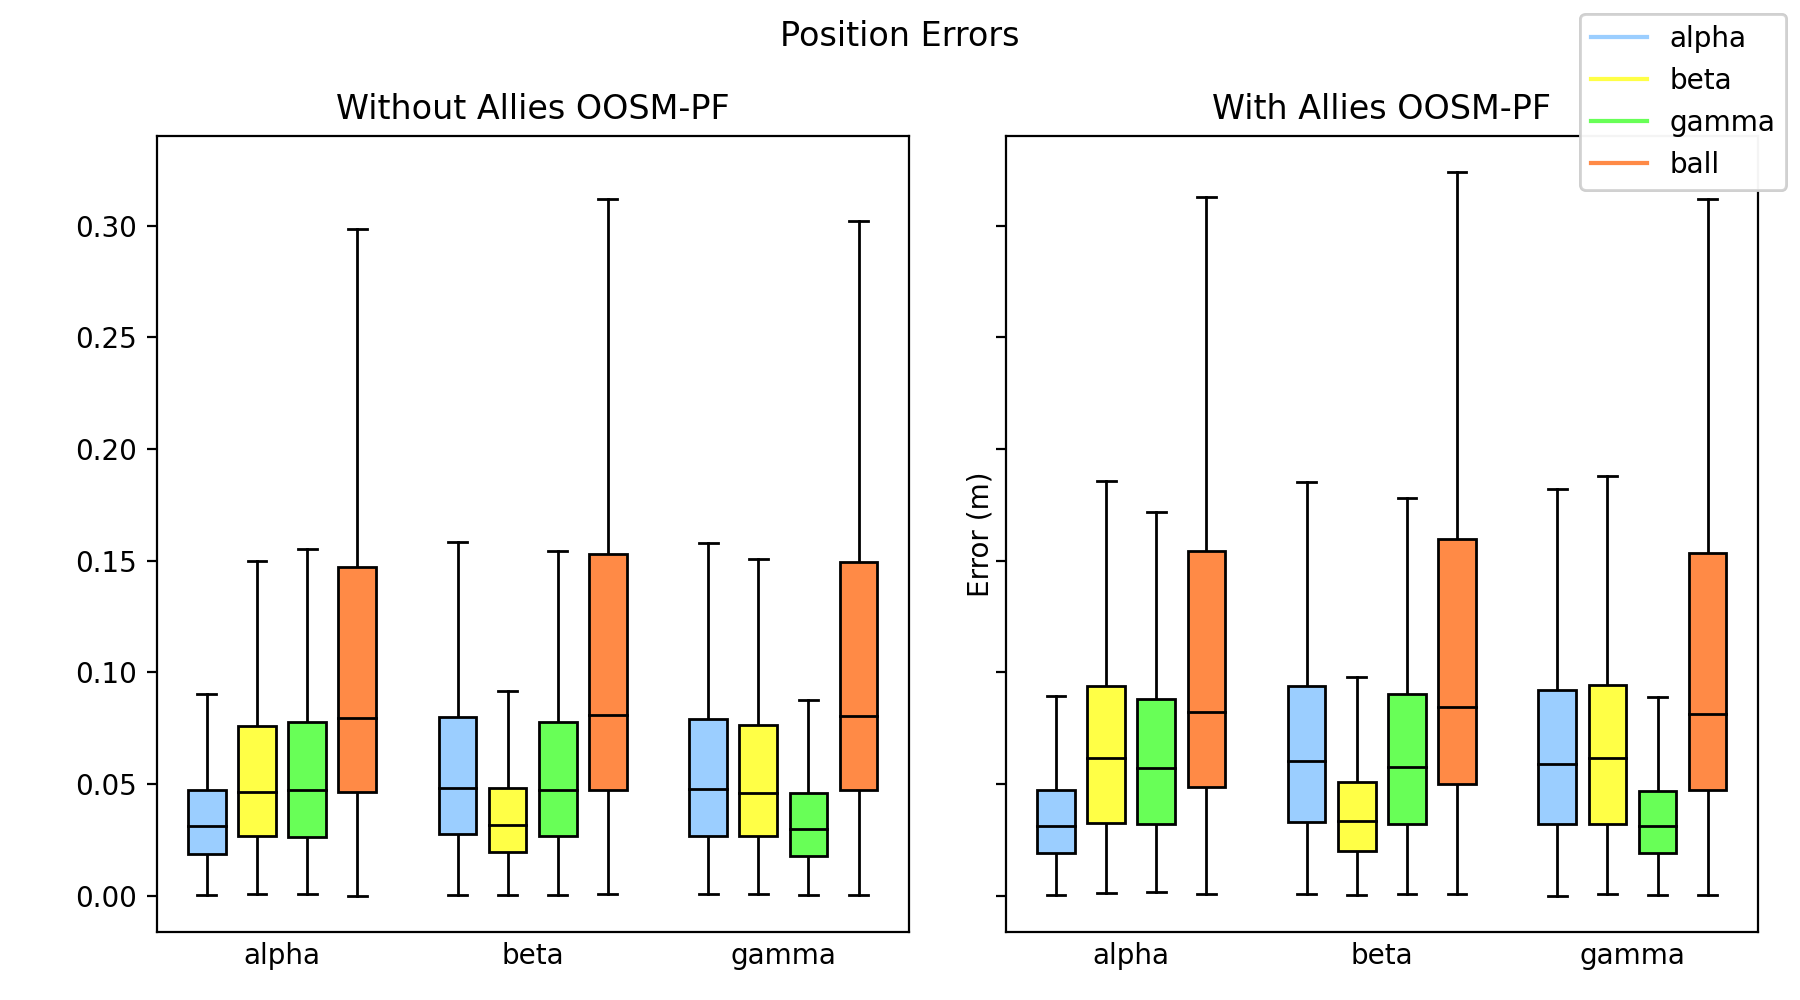
\includegraphics[width=0.9\textwidth]{resources/cfg1_AS_AT_error_pos.png}
    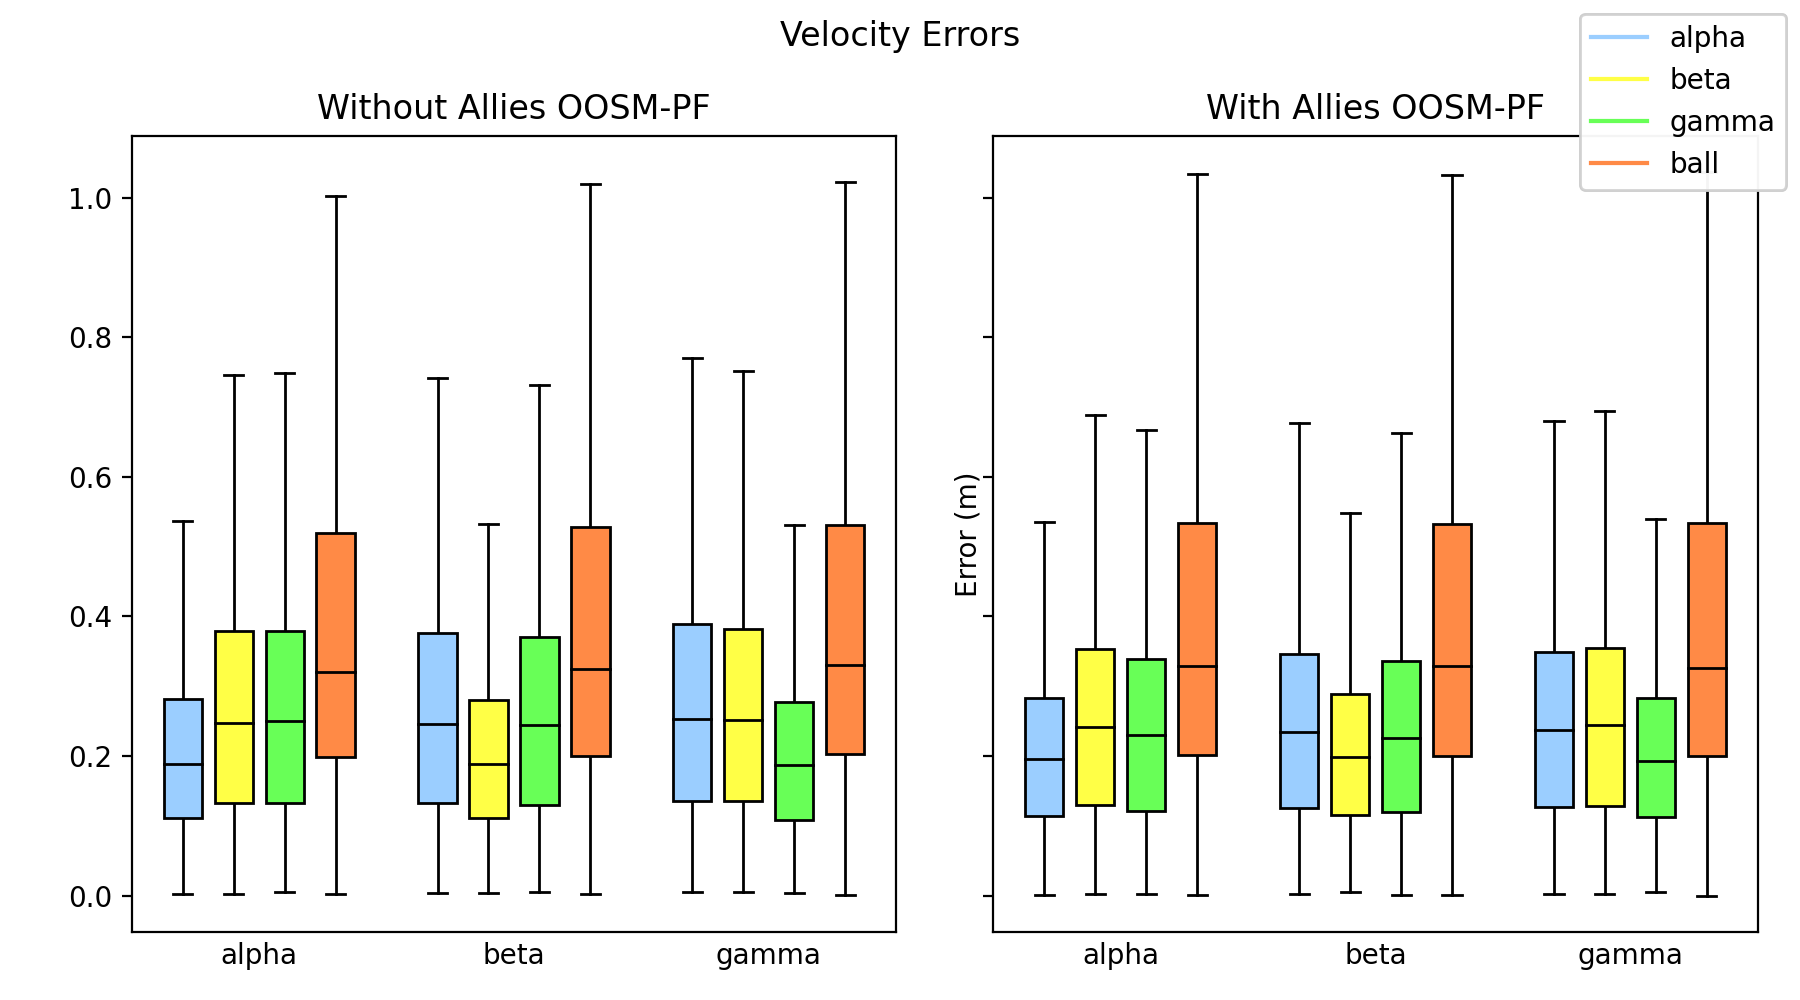
\includegraphics[width=0.9\textwidth]{resources/cfg1_AS_AT_error_vel.png}
    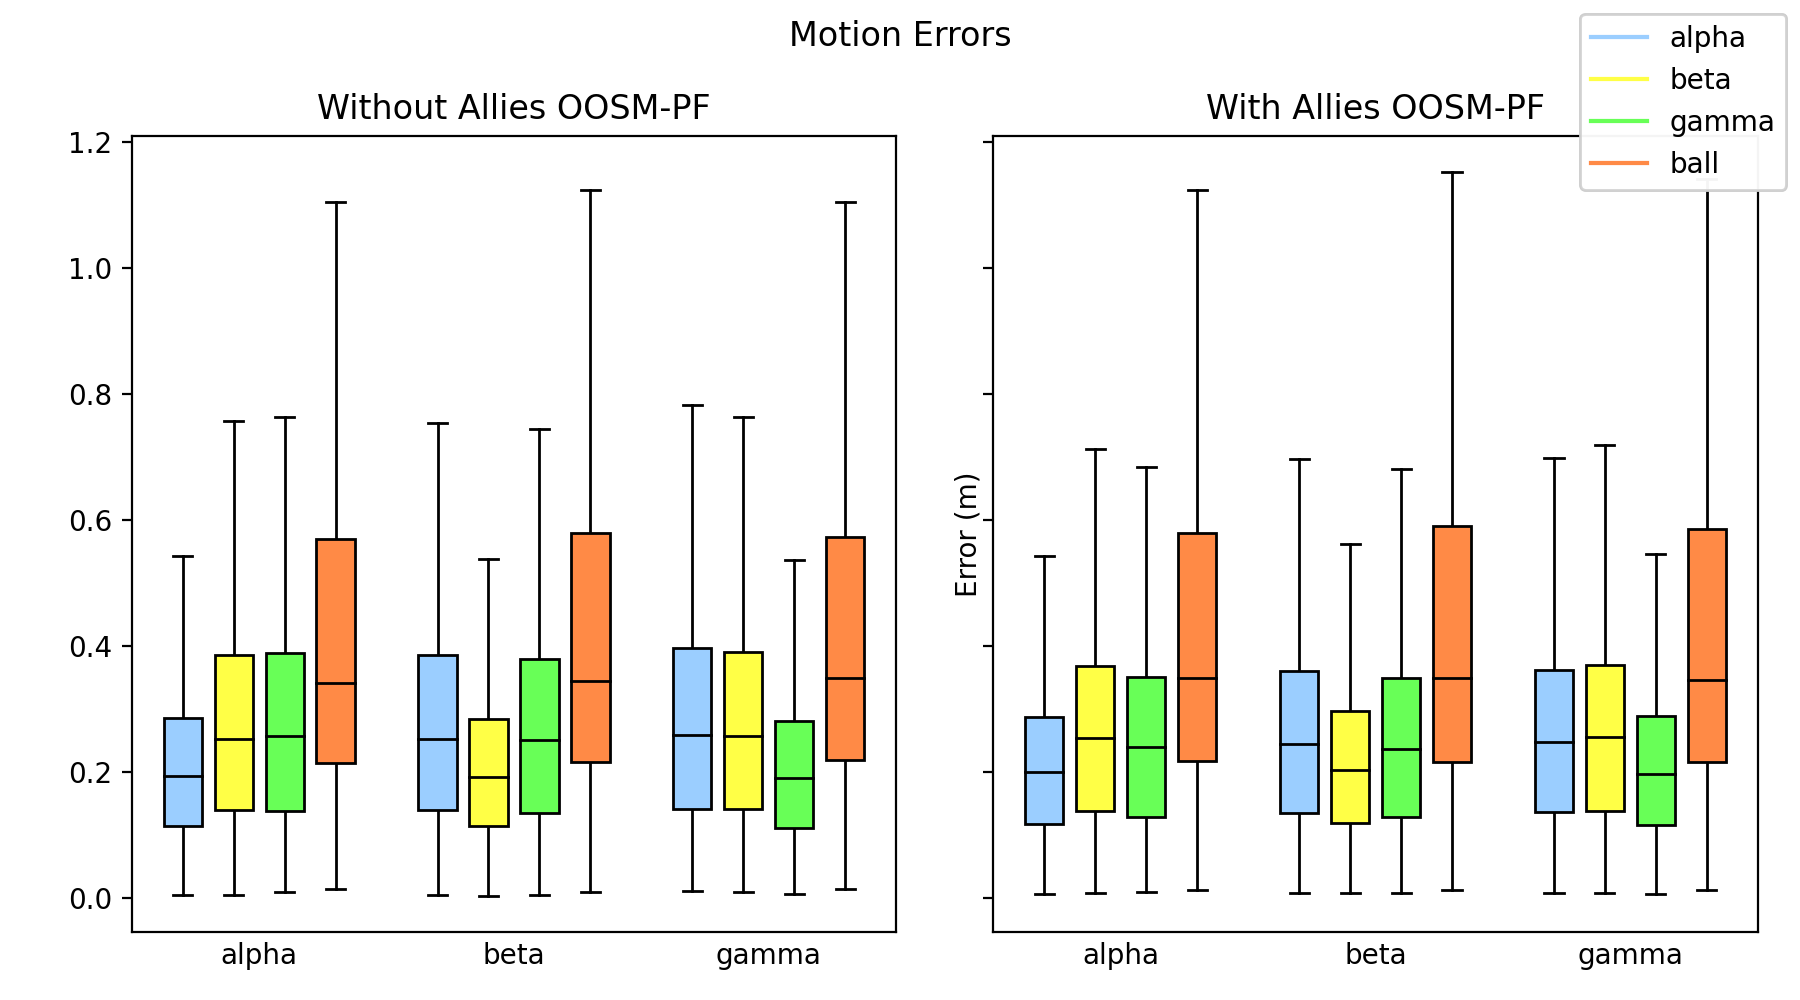
\includegraphics[width=0.9\textwidth]{resources/cfg1_AS_AT_error_motion.png}
    \caption{\textit{Error} \textit{world model} S dan T jaringan baik}
    \label{fig:1-s-t-error}
    \bigskip
\end{figure}

\begin{figure}[p]
    \centering
    \medskip
    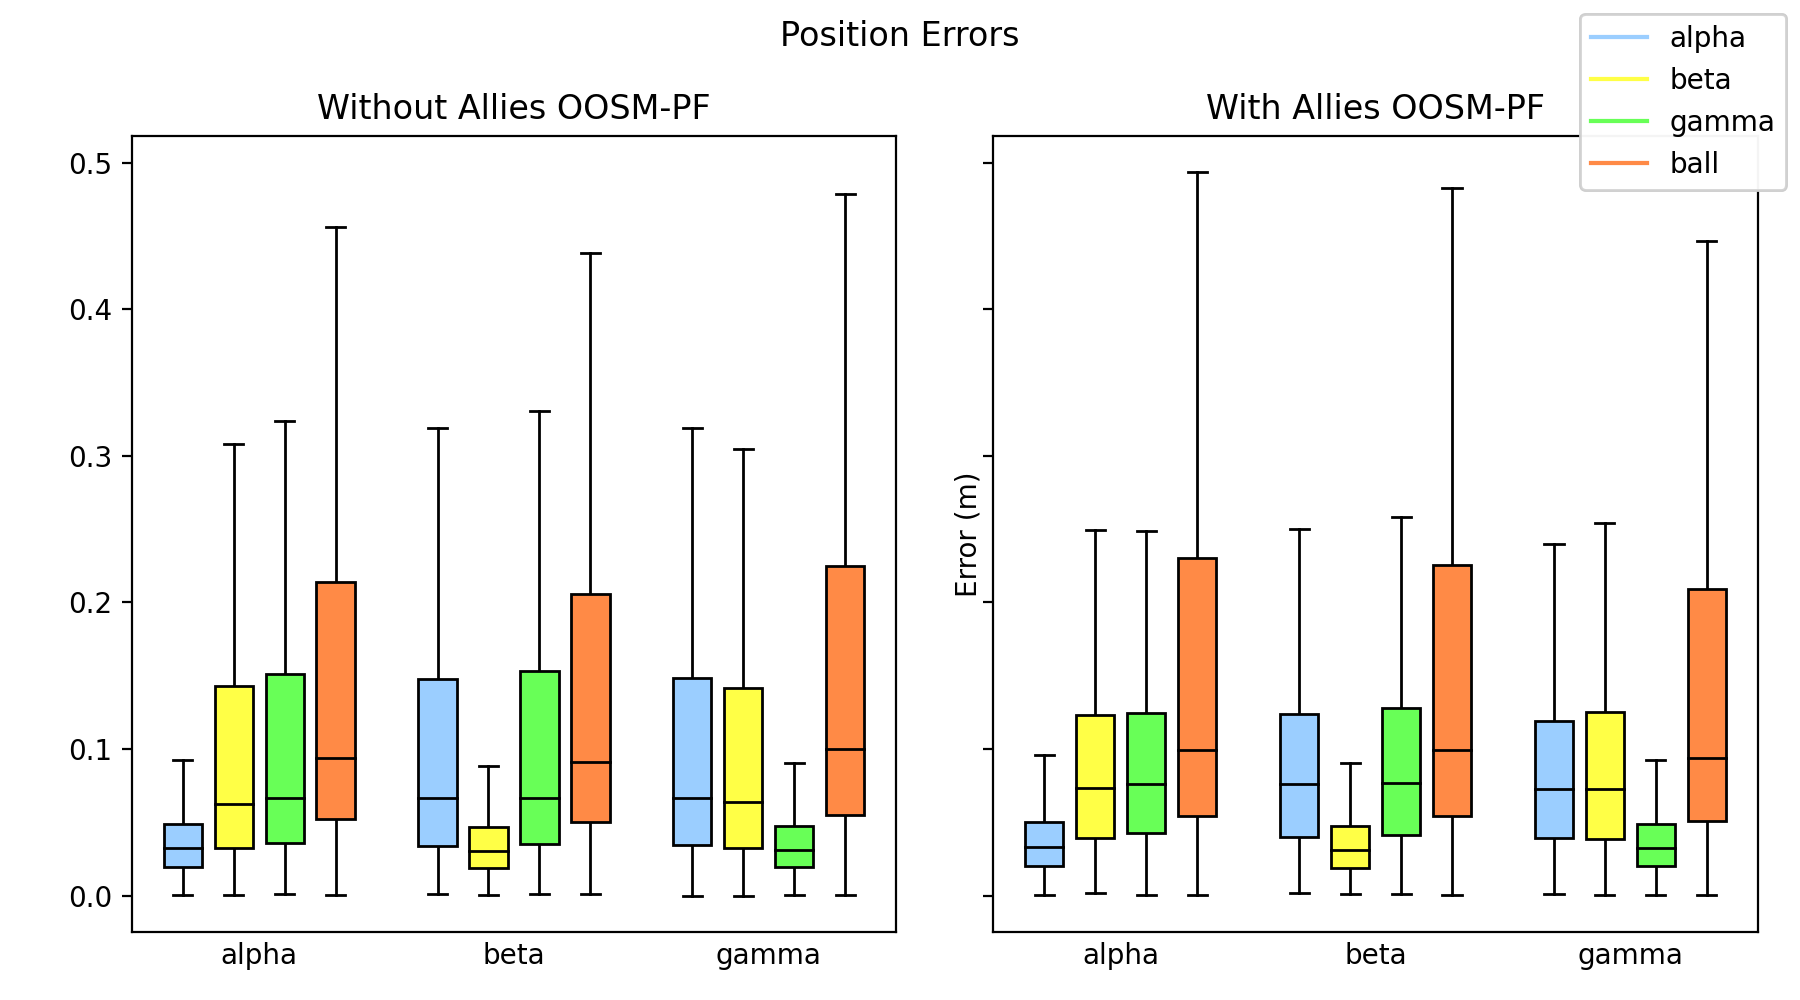
\includegraphics[width=0.9\textwidth]{resources/cfg2_AS_AT_error_pos.png}
    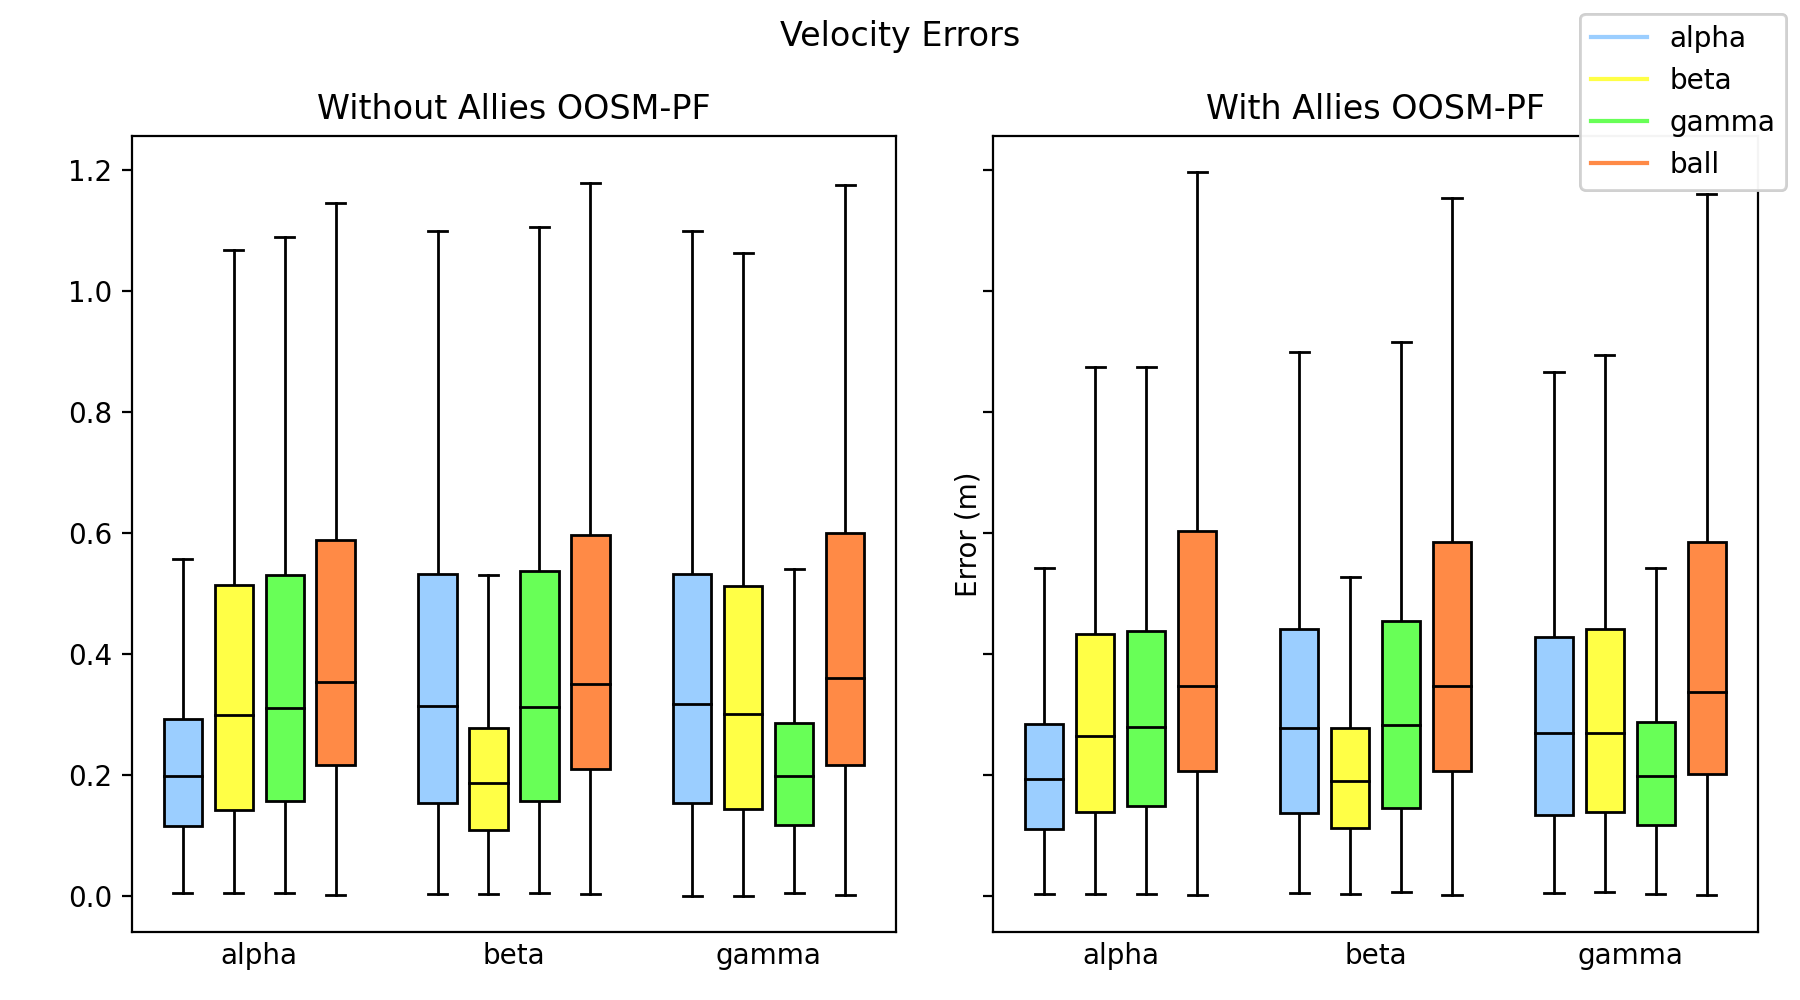
\includegraphics[width=0.9\textwidth]{resources/cfg2_AS_AT_error_vel.png}
    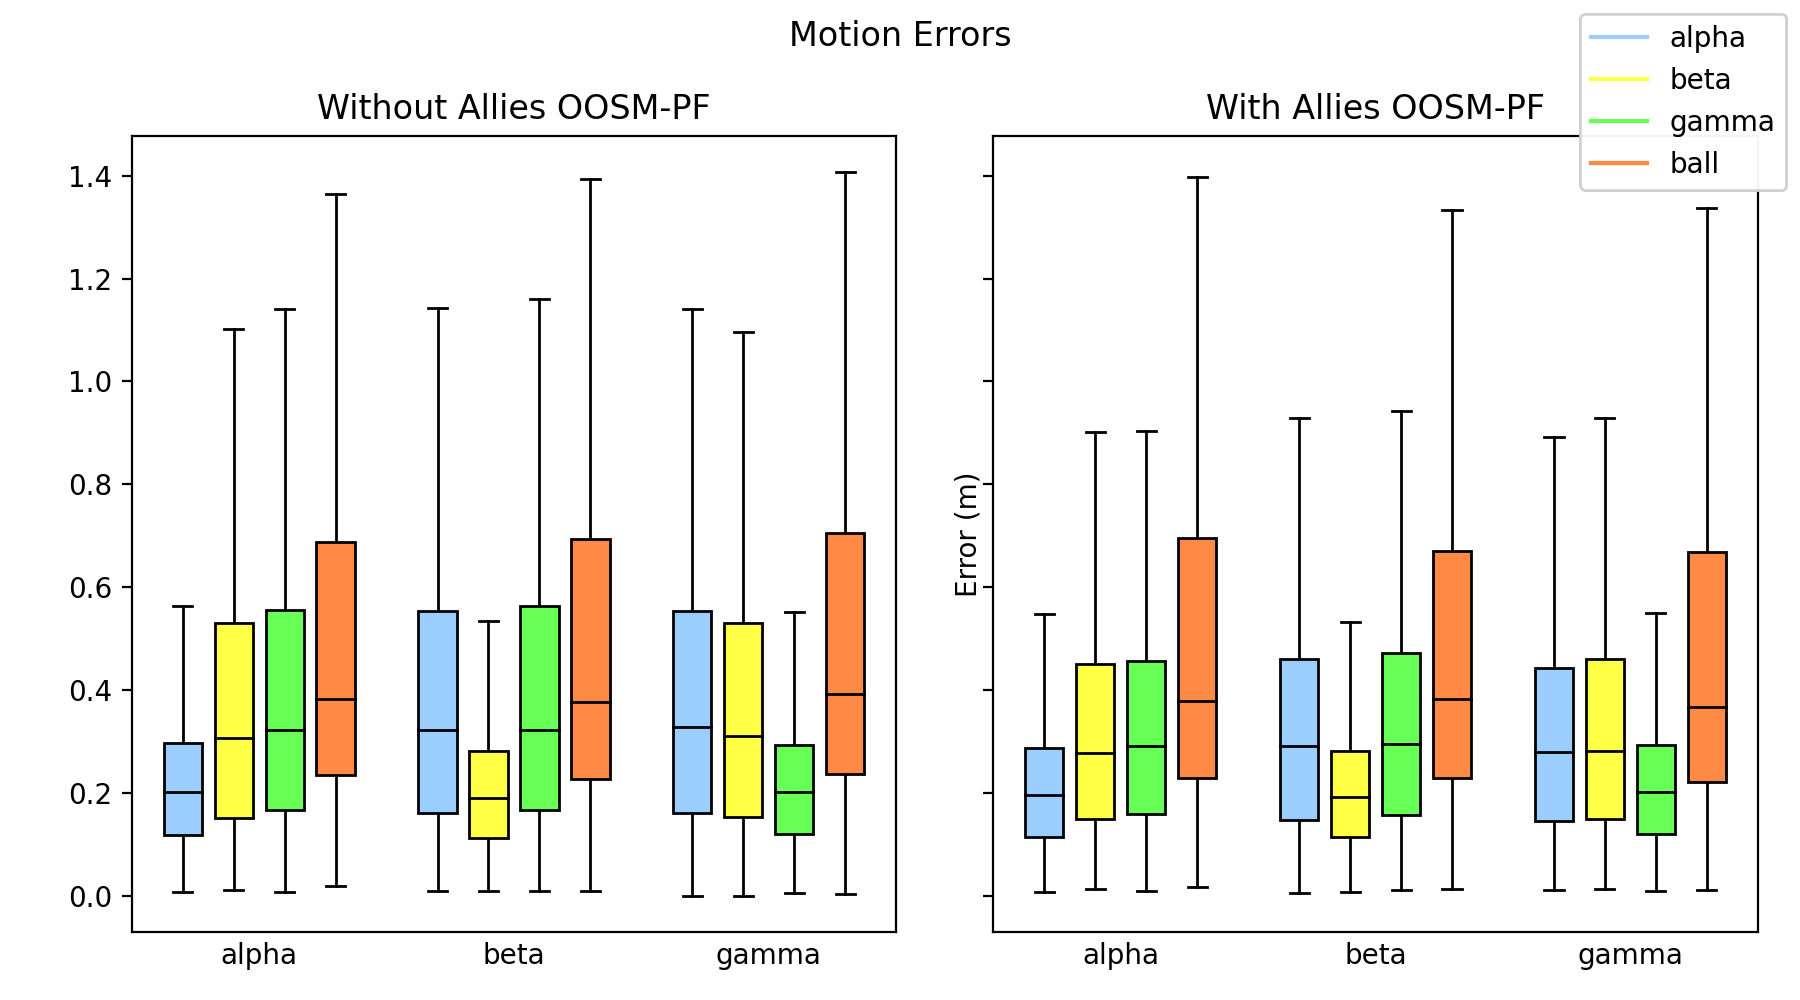
\includegraphics[width=0.9\textwidth]{resources/cfg2_AS_AT_error_motion.png}
    \caption{\textit{Error} \textit{world model} S dan T jaringan sedang}
    \label{fig:2-s-t-error}
    \bigskip
\end{figure}

\begin{figure}[p]
    \centering
    \medskip
    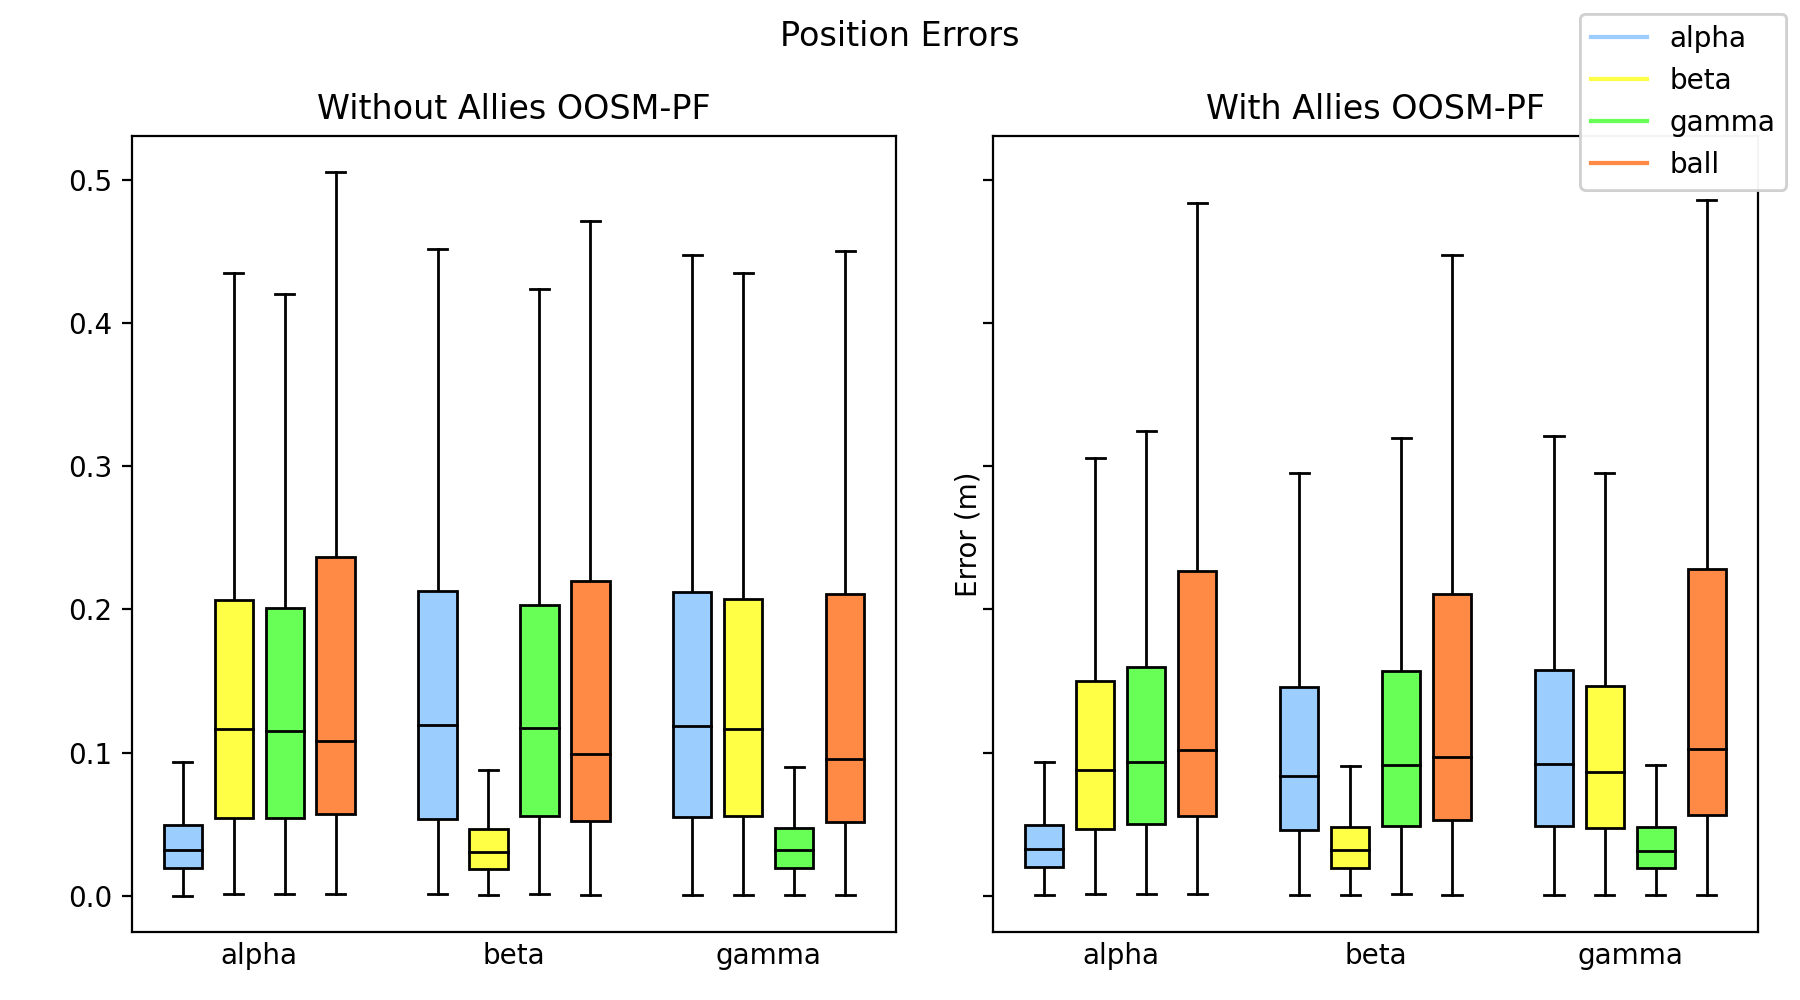
\includegraphics[width=0.9\textwidth]{resources/cfg3_AS_AT_error_pos.png}
    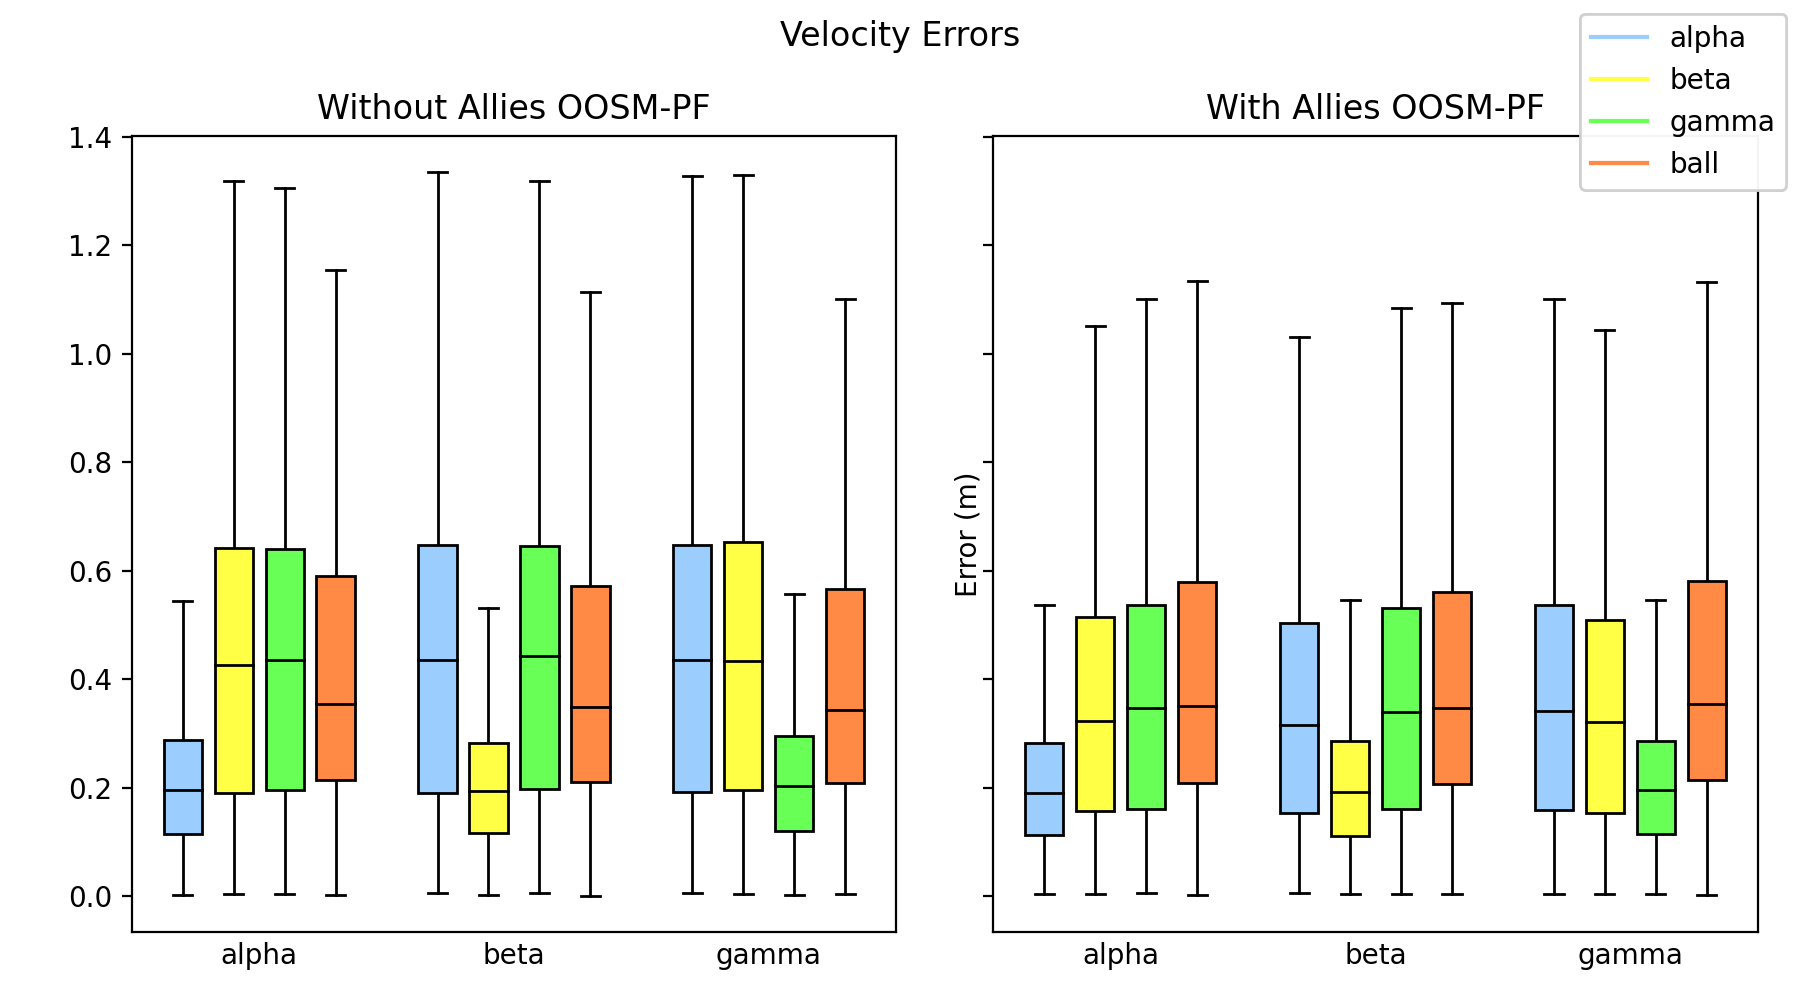
\includegraphics[width=0.9\textwidth]{resources/cfg3_AS_AT_error_vel.png}
    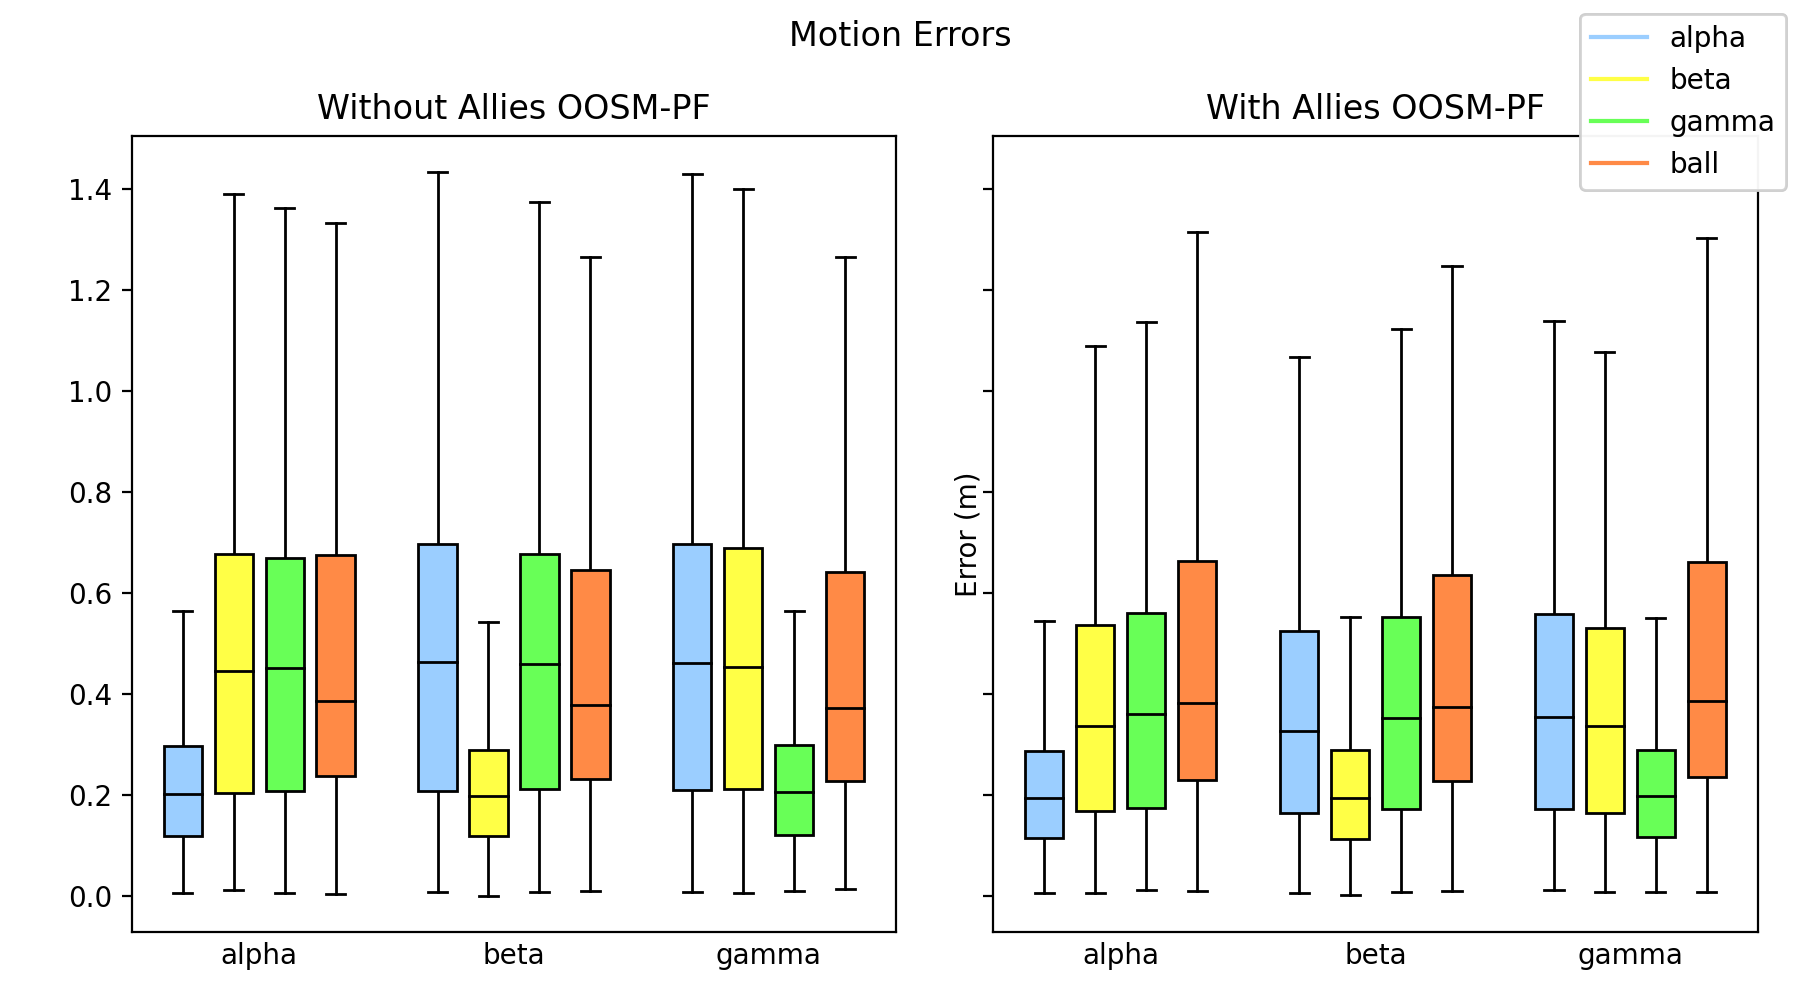
\includegraphics[width=0.9\textwidth]{resources/cfg3_AS_AT_error_motion.png}
    \caption{\textit{Error} \textit{world model} S dan T jaringan buruk}
    \label{fig:3-s-t-error}
    \bigskip
\end{figure}

Pada grafik \ref{fig:1-s-t-error}, hasil estimasi posisi dan kecepatan dari robot teman sedikit memburuk. Hal ini dikarenakan hasil persepsi \textit{vision} yang lebih \textit{noisy} dibandingkan dengan hasil lokalisasi yang menggunakan beberapa sensor berbeda. Sedangkan pada grafik \ref{fig:2-s-t-error} dan \ref{fig:3-s-t-error}, koreksi robot teman dapat membantu meningkatkan akurasi estimasi posisi dan kecepatan karena persepsi \textit{vision} yang lebih tersedia dibandingkan menunggu informasi dari robot teman yang terlambat.

\chapter{PENUTUP}

Bab ini memaparkan hasil-hasil simpulan yang dapat ditarik berdasarkan uji coba beserta saran yang dapat diambil untuk pengembangan-pengembangan berikutnya.

\section{Simpulan}

Berdasarkan hasil eksperimen yang diperoleh, didapatkan bahwa algoritma estimasi gerakan robot tim dan bola yang paling akurat adalah algoritma yang:
\begin{enumerate}
    \item Menggunakan algoritma AMCL berbasis \textit{pose} dan \textit{twist} untuk mengestimasi gerakan robot sendiri
    \item Menggunakan algoritma penapis partikel dengan penanganan data terlambat untuk mengestimasi gerakan bola
    \item Menggunakan algoritma penapis partikel dengan penanganan data terlambat untuk mengestimasi dan mengoreksi gerakan robot teman
    \item Mengoreksi hasil estimasi berdasarkan selisih waktu sekarang dengan \textit{timestamp} data terakhir
\end{enumerate}

Konfigurasi-konfigurasi tersebut mempunyai kinerja yang lebih baik dibandingkan dengan alternatif seperti menggunakan AMCL berbasis \textit{pose} saja atau estimasi gerakan bola menggunakan penapis Kalman.

\section{Saran}

Saran yang dapat diterapkan untuk pengembangan-pengembangan berikutnya diantaranya adalah:
\begin{enumerate}
    \item Memvalidasi hasil uji coba dengan percobaan langsung di lingkungan nyata dengan robot di lapangan atau menggunakan data yang diambil dari uji coba robot di lapangan
    \item Melakukan koreksi posisi robot teman menggunakan persepsi \textit{vision} terhadap teman tersebut
    \item Menyebarkan seluruh distribusi estimasi dibandingkan hanya estimasinya saja melalui komunikasi
    \item Menerapkan berbagai variasi modifikasi penapis Kalman yang ada
\end{enumerate}

%----------------------------------------------------------------%

\begingroup
\renewcommand{\baselinestretch}{1.0}
\printbibliography[heading=bibintoc]
\endgroup

% Format judul bab lampiran
% \titleformat{\chapter}[hang]
%   {\large\bfseries}
%   {\chaptertitlename\ \thechapter}{1em}
%     {\large\bfseries}
% \titlespacing*{\chapter}{0pt}{-1.5\baselineskip}{\parskip}

% \begin{appendices}
%     \input{chapters/appendix-1}
%     \input{chapters/appendix-2}
% \end{appendices}

\end{document}
